%%  
%%  This is the file that controls everything - maxima.tex
%%
%%
%%  Initialization Stuff
\documentclass[oneside,english]{book}
\usepackage{pslatex} %%Used pslatex here because the maxima examples 
                     %%fit properly on the page in a PDF document
\usepackage[T1]{fontenc}
\usepackage[latin1]{inputenc}
\usepackage{geometry}
\usepackage{multicol}
\geometry{verbose,letterpaper,tmargin=1in,bmargin=1in,lmargin=1in,rmargin=1in}
\usepackage{babel}
\usepackage{makeidx}
\makeindex
\usepackage{emaxima}
\maximatexsessionbaselineskip = 0pt
\usepackage{graphics}
\usepackage{rotating}
\usepackage{color}
%\usepackage{mathtime}
\usepackage{titlesec}
\usepackage{thumbpdf}

\ifx\pdfoutput\undefined
     \usepackage[backref=false,
                 colorlinks=false,
                 breaklinks=true,
                 hyperindex=false]{hyperref}
%       \usepackage[dvips]{graphicx}
%               \DeclareGraphicsExtensions{.eps,.ps,.bmp,.tif,.tiff,.tga}  
%               \graphicspath{{EPS/}}
  \else
%       \usepackage[pdftex]{graphicx}
%               \pdfcompresslevel=9
%               \DeclareGraphicsExtensions{.jpg,.pdf,.mps,.png} 
%               \graphicspath{{PDF/}}
     \usepackage[pdftex=true,
                     plainpages=false,
                 backref=section,
                 colorlinks=true,
                 breaklinks=true,
%                 hyperindex=true,
                 hyperindex=false,
                 pdfpagelabels, 
%--------- Cropping -----------------------------------------------------------
% For on-line PDF generation only.
%        pdfpagescrop={98 100 512 692},
%-------- Better Color for Links ----------------------------------------------
%        linkcolor=webgreen,
%        citecolor=webgreen,
%        filecolor=webbrown,
%------ Doc Info --------------------------------------------------------------
        pdftitle={The Maxima Book},
        pdfauthor={Paulo Ney de Souza, Richard Fateman, Joel Moses, Cliff Yapp},
        pdfsubject={Maxima},
        pdfkeywords={Maxima, Macsyma, CAS, Symbolic Computation},
        pdfproducer={pdfTeX 0.14e},
        pdfcreator={LaTeX + Hyperref},
%------ Doc View --------------------------------------------------------------
        bookmarksopen=false,
        pdfnewwindow=true,
%
%       The following option controls how the document is initially displayed
%       in viewers - the whole page visible, fit width, etc.  Here are the
%       various options:
%       Fit    fit whole page in window
%       FitH   fit whole width of page 
%       FitV   fit whole height of page 
%       FitB   fit whole "Bounding Box" page 
%       FitBH  fit whole width of "Bounding Box" of page 
%       FitBV  fit whole height of "Bounding Box" of page 
%
        pdfstartview=FitH,
%
        pdfpagemode=UseOutlines]{hyperref}
%------ Fill in deficiencies of Hyperref --------------------------------------
        \pdfinfo{ 
              /CreationDate (D:20010321000000)
              /ModDate      (D:20010321000000) }
\fi

\definecolor{webgreen}{rgb}{0,.5,0}
\definecolor{webbrown}{rgb}{.6,0,0}
\definecolor{webyellow}{rgb}{0.98,0.92,0.73}

%------------ These are the fancy Chapter and Section headings:
\renewcommand{\thechapter}{\arabic{chapter}}
\titleformat{\chapter}[display]
{\bfseries\Large}
{\filleft\MakeUppercase{\chaptername} \Huge\thechapter}
{4ex}
{\titlerule
\vspace{2ex}%
\filright}
[\vspace{2ex}%
\titlerule]

\titleformat{\section}%[block]
{\large\sffamily}
{\bfseries\thesection}{.5em}{\bfseries}

\titleformat{\subsection}
%{\titlerule
{
\vspace{.8ex}%
\normalfont\itshape\bfseries}
{\hskip1cm\thesubsection.}{.5em}{}
%--------- End of fancy headings for Chapter and Sections ...


% Name of the program:
\newcommand{\maxi}{maxima}
\newcommand{\Max}{Maxima}
\newcommand{\maxp}{m\ae{}xim\raisebox{1.0ex}{\begin{turn}{-180}e\end{turn}}}

% Some custom definitions
\newdimen\firstcol
\firstcol=.35\textwidth
\newdimen\secondcol
\secondcol=.65\textwidth

\begin{document}

\title{The Maxima Book}

\author{Paulo Ney de Souza\\
        Richard J. Fateman \\
                Joel Moses \\
                Cliff Yapp}
                

\maketitle

\subsection*{Credits}

~

Paulo Ney de Souza

Jay Belanger

Richard Fateman

Joel Moses

Cliff Yapp\\
\newpage


\tableofcontents
\newpage

\addcontentsline{toc}{part}{Preface}
 Many hands and minds have contributed to Macsyma, in developing
it as a research program, and tuning it for use by others.
We have enjoyed constructing
Macsyma and we hope that you will enjoy using it.
We hope you will consider
contributing your carefully polished and documented
application programs to libraries at your local installation and
other sites.


\subsection*{Examples}
\begin{multicols}{2}
\begin{tabbing}
1. First Example~~~~~~~~~~~~~~~~~~~~~~~~~~~~~~~~~~~\= \pageref{Example1} \\
2. Quitting Maxima \>\pageref{Quitting Maxima (Example 2)}\\
3. End of Entry Characters \>\pageref{End of Entry Characters (Example 3)}\\
4. Line Labels \>\pageref{Line Labels (Example 4)}\\
5. Labeling an Example Equation \>\pageref{Labeling an Equation (Example 5)}\\
6. Evaluation Toggle \>\pageref{Evaluation Toggle (Example 6)} \\
7. Basic Use of ev Command \>\pageref{Basic Use of ev Command (Example 7)}\\
8. ev's Expand Option \>\pageref{ev's Expand Option (Example 8)}\\
9. Float Example \>\pageref{FLOAT example (Example 9)}\\
\end{tabbing}
\end{multicols}

\part{The Maxima Program and Standard Packages}

\chapter{Introduction}
  
\section{What is Maxima?}

Maxima (pronounced \maxp\footnote{The acronym \Max\ is the corruption of the main project name MACSYMA, which  stands for Project MAC's 
SYmbolic MAnipulation System. {\it MAC} itself is an acronym, usually 
cited as meaning Man and Computer or Machine Aided Cognition. The
Laboratory for Computer Science at the Massachusetts Institute of Technology
was known as Project MAC during the initial development of MACSYMA.  The name
MACSYMA is now trademarked by Macsyma Inc.})
is a large computer program designed for the manipulation
of algebraic expressions. You can use \Max\
for manipulation of algebraic expressions involving
constants, variables, and functions. It can
differentiate, integrate, take limits, solve equations,
factor polynomials, expand functions in power series, solve differential 
equations in closed form, and perform many other
operations.  It also has a programming language that you can use to 
extend Maxima's capabilities.


\subsection*{The Dangers of Computer Algebra}

~

With all this marvelous capability, however, you must bear in mind the 
limitations inherent in any such tool.  Those considering the use of 
computers to do mathematics, particularly
students, must be warned that these systems are no substitute for
hands on work with equations and struggling with concepts. These systems
do not build your mathematical intuition, nor will they strengthen
your core skills. This will matter a great deal down the road, especially
to those of you who wish to break new ground in theoretical mathematics
and science. Do not use a computer as a substitute for your basic
education.

By the same token, however, proficiency with computers and computer
based mathematics is crucial for attacking the many problems which
literally cannot be solved by pencil and paper methods. In many cases
problems which would take years by hand can be reduced to seconds
by powerful computers. Also, in the course of a long derivation, it
is sometimes useful for those who have already mastered the fundamentals
to do work in these systems as a guard against careless errors, or
a faster means than a table of deriving some particular result. Also,
in case of an error, fixing the resulting error can often be much
quicker and simpler courtesy of a mathematical notebook, which can
be reevaluated with the correct parameters in place.

But just as a computer can guard against human error, the human must
not trust the computer unquestioningly. All of these systems have
limits, and when those limits are reached it is quite possible for
bizarre errors to result, or in some cases answers which are actually
wrong, to say nothing of the fact that the people who programmed these
systems were human, and make mistakes. To illustrate the limits of
computer algebra systems, we take the following example: when given the 
integral \verb@Integrate 1/sqrt(2-2*cos(x))@ \verb@from x=-pi/2 to pi/2@, 
Mathematica 4.1 gives, with no warnings, \verb@\!\(2\ Log[4] - 2\ Log[Cos[\[Pi]\/8]]@
\verb@+ 2\ Log[Sin[\[Pi]\/8]]\)@ which \verb@N[%]@ evalutates numerically to
give 1.00984.  Maxima 5.6 returns the integral unevaluated, the commercial 
Macsyma says the integral is divergent, and Maple 7 says infinity. (Cite Maxima
Email list here.)
Had the person who wished to learn the result blindly trusted most of the 
systems in question, he might have been misled. So remember to think about 
the results you are given. The computer is not always necessarily right,
and even if it gives a correct answer that answer is not necessarily complete.

\section{A Brief History of Macsyma}
\label{history}

The birthplace of Macsyma, where much of the original coding took place, was
Project MAC at MIT in the late 1960s and earlier 1970s. Project MAC was an MIT
research unit, which was folded into the current Laboratory for Computer 
Science.  Research support for Macsyma included the Advanced Research Projects 
Agency(ARPA), Department of Defense, the US Department of Energy, and other 
government and private sources.

The original idea, first voiced by Marvin Minsky, was to automate the kinds 
of manipulations done by mathematicians, as a step toward understanding the
power of computers to exhibit a kind of intelligent behavior. \cite{MAC-M-124}
The undertaking grew out of a previous effort at MITRE Corp called Mathlab, 
work of Carl Engelman and others, plus the MIT thesis work of Joel Moses on 
symbolic integration, and the MIT thesis work of William A. Martin. The new
effort was dubbed Macsyma - Project MAC's SYmbolic MAnipulator. The original 
core design was done in July 1968, and coding began in July 1969. This was long
before the days of personal computers and cheap memory - initial development 
was centered around a single computer shared with the Artificial Intelligence 
laboratory, a DEC PDP-6.  This was replaced by newer more powerful machines 
over the years, and eventually the Mathlab group acquired its own DEC-PDP-10, 
MIT-ML running the ITS operating system. This machine became a host on the 
early ARPANET, predecessor to the internet, which helped it gain a
wider audience. As the effort grew in scope and ability the general
interest it created led to attempts to "port" the code - that is, to
take the series of instructions which had been written for one machine
and operating system and adapt them to run on another, different 
system. The earliest such effort was the running of Macsyma in a MacLisp 
environment on a GE/Honeywell Multics mainframe, another system
at MIT. The Multics environment provided essentially unlimited address
space, but for various reasons the system was not favored by 
programmers and the Multics implementation was never popular.
The next effort came about when a group at MIT designed and implemented a machine
which was based on the notion that hardware support of Lisp would make
it possible to overcome problems that inhibited the solution of
many interesting problems.  The Lisp machine clearly had to support 
Macsyma, the largest Lisp program of the day, and the effort paid off with 
probably the best environment for Macsyma to date (although requiring something
of an expert perspective).  Lisp machines, as well as other special
purpose hardware, tended to become slow and expensive compared to
off-the-shelf machines built around merchant-semiconductor CPUs, and
so the two companies that were spun off from MIT (Symbolics Inc, and 
LMI) both eventually disappeared.  Texas Instruments built a machine called
the Explorer bases on the LMI design, but also stopped production.

Around 1980, the idea of porting Macsyma began to be more interesting,
and the Unix based vaxima distribution, which ran on a Lisp system 
built at the University of California at Berkeley for VAX UNIX demonstrated 
that it was both possible and practical to run the software on less expensive 
systems.  (This system, Franz Lisp, was implemented primarily in Lisp with 
some parts written in C.) Once the code stabilized, the new version opened up 
porting possibilities, ultimately producing at least six variations on the 
theme which included Macsyma, Maxima, Paramax/Paramacs, Punimax, Aljbar, and 
Vaxima.  These have followed somewhat different paths, and most were destined 
to fade into the sunset.  The two which survived obscurity, Maxima and 
Macsyma, we will discuss below.  Punimax was actually an offshoot of Maxima - 
some time around 1994 Bruno Haible (author of clisp) ported maxima to clisp.
Due to the legal concerns of Richard Petti, then the owner of the commercial
Macsyma, the name was changed to Punimax.  It has not seen much activity since
the initial port, and although it is still available the ability of the main
Maxima distribution to compile on Clisp makes further development of 
Punimax unlikely.

 There is a certain surprising aspect in this multiplicity of versions
and platforms, given how the code seemed tied to the development environment,
which included a unique operating system.  Fortunately, Berkeley's building 
a replica of the Maclisp environment on the MIT-ML PDP-10, using tools 
available in almost any UNIX/C environment, helped solve this problem.
Complicating the matter was the eventual demise of the PDP-10 and 
Maclisp systems as Common Lisp (resembling lisp-machine lisp), influenced by 
BBN lisp and researchers at Stanford, Carnegie Mellon University, and Xerox, began to take 
hold.  It seemed sensible to re-target
the code to make it compatible with what eventually
became the ANSI Common Lisp standard.  Since almost everything needed for
for Macsyma can be done in ANSI CL, the trend toward standardization 
made many things simpler.  There are a few places
where the language is not standardized, in particular connecting to
modules written in other languages, but much of the power of the
system can be expressed within ANSI CL. It is a trend the Maxima
project is planning to carry on, to maintain and expand on this
flexibility which has emerged.

 With all these versions, in recent history there are two which have
been major players, due this time more to economics than to code
quality.  1982 was a watershed year in many respects for Macsyma - it
marks clearly the branching of Macsyma into two distinct products, 
and ultimately gave rise to the events which have made Maxima both 
possible and desirable.  MIT had decided, with the gradual spread of 
computers throughout the academic world, to put Macsyma on the market
commercially, using as a marketing partner the firm of  Arthur D. Little, Inc.
This version was sold to the Symbolics Inc., which, depending on your 
perspective, either turned the project into a significant marketing effort
to help sell their high-priced lisp machines, or was a diversionary
tactic to deny their competitors (LMI) this program.  At the same
time MIT forced UC Berkeley (Richard Fateman) to withdraw the
copies from about 50 sites of the VAX/UNIX and VAX/VMS versions
of Macsyma that he had distributed with MIT's consent, until some 
agreement could be reached for technology transfer. Symbolics hired some of 
the MIT staff to work at Symbolics in order to improve the code,which was 
now proprietary. The MIT-ML PDP-10 also went
off the Arpanet in 1983. (Interestingly, the closing of the MIT Lisp
and Macsyma efforts was a key reason Richard Stallman decided to form
the Free Software Foundation.)  Between the high prices, closed 
source code, and neglecting all platforms in favor of Lisp Machines  
pressure came to bear on MIT to release another version to accommodate 
these needs, which they did with some reluctance.  The new version was distributed
via the National Energy Software Center, and called DOE Macsyma. It 
had been re-coded in a dialect of lisp written for the VAX at MIT
called NIL. There was never a complete implementation. At about the 
same time a VAX/UNIX version "VAXIMA" was put into the same library by 
Berkeley. This ran on any of hundreds of machines running the Berkeley version of 
VAX Unix, and through a UNIX simulator on VMS, on any VAX system.
The DOE versions formed the basis of the subsequent non-Symbolics 
distributions. The code was made available through the National Energy
Software Center, which in its attempt to recoup its costs, charged
a significant fee \verb@($1-2k?).@  It provided full source, but in a 
concession to MIT, did not allow redistribution.  This prohibition seems 
to have been disregarded, and especially so since NESC disappeared.  Perhaps 
it didn't recoup its costs! Among all the new activity centered around DOE 
Macsyma, Prof. William Schelter began maintaining 
a version of the code at UT Austin, calling his variation Maxima. He
refreshed the NESC version with a common-lisp compatible code version.


There were, from the earliest days, other computer algebra systems
including Reduce, CAMAL, Mathlab-68, PM, and ALTRAN.  More 
serious competition, however, did not arrive until Maple and Mathematica were
released, Maple in 1985 (Cite list of dates) and Mathematica in 1988 (cite 
wolfram website). These systems were inspired by Macsyma in terms of their 
capabilities, but they proved to be much better at the challenge of building
mind-share.  DOE-Macsyma, because of the nature of its users and maintainers, never 
responded to this challenge. Symbolics' successor Macsyma Inc, having 
lost market share and unable to meet its expenses, was sold in the summer of 
1999 after attempts to find endowment and academic buyers failed. (Cite Richard
Petti usenet post.)  The purchaser withdrew Macsyma from the market 
and the developers and maintainers of that system dispersed. Mathematica and Maple
appeared to have vanquished Macsyma.

It was at this point Maxima re-entered the game.  Although it was not
widely known in the general academic public, W. Schelter had been
maintaining and extending his copy of the code ever since 1982. He 
had decided to see what he could do about distributing it more widely.  
He attempted to contact the NESC to request permission to distribute
derivative works.  The duties of the NESC had been assumed in 1991 by
the Energy Science and Technology Software Center, which granted him
virtually unlimited license to make and distribute derivative works,
with some minor export related caveats.  

It was a significant breakthrough.  While Schelter's code had been available 
for downloading for years, this 
activity became legal with the release from DOE granted in Oct. 1998, and
Maxima began to attract more attention.  
When the Macsyma company abruptly vanished in 1999, with no warning or
explanation, it left their customer base hanging.  They began looking
for a solution, and some drifted toward Maxima.

Dr. Schelter maintained the Maxima system until his untimely death in
July, 2001. It was a hard and unexpected blow, but Schelter's obtaining
the go-ahead to release the source code saved the project and possibly
even the Macsyma system itself. A group of users and developers who 
had been brought together by the email list for Maxima decided to try and
form a working open source project around the Maxima system, rather
than let it fade - which is where we are today.



\chapter{Installing}
  
\section{Installing on Linux}

Note:  This is written for version 5.6.  With 5.9 things should change
significantly, both for Windows and Linux, so a rewrite will be performed
at that time.

\subsection{The Easy Way}

If you are using Debian Linux, there are packages for Maxima in the
Debian archives. Redhat users can find packages at rpmfind.net and
mirrors. To the best of my knowledge these packages are all compiled
against GNU Common Lisp (GCL). GCL does not access the readline library,
which makes using Maxima on the terminal somewhat cumbersome. There
are various interfaces which address this issue, but in the case of
these packages the left arrow key will not take you back to the middle
of an expression and let you edit just what you want - you will have
to delete everything back to the point where you made your error.
See the interfaces section for more about this, or if you really want
to use maxima in the terminal I'd recommend compiling against CLISP. 


\subsection{The Hard Way}

Compiling Maxima on Linux should go reasonably smoothly, although
some distributions seem to have problems with the makefiles. Redhat
7.1 is known to be a bit flaky in this regard.


\subsubsection{Compiling with GCL\index{Compiling!GCL} }

GCL is the version of Lisp Maxima has been maintained on for many
years by William Schelter, and thus the default system on which to
build Maxima. Maxima will typically be made to work with GCL, and
then be fixed to work with other Lisps. If in doubt, start here, but
again be warned that readline support is not present in GCL.

The first step in this process is to compile GCL. The files from the
compiling of GCL are needed when building Maxima against it, so first
download and decompress the most current version of GCL. Compiling
it should be simple:

\vspace{3ex}


cd \$HOME/gcl

./configure

make\vspace{3ex}


Once that is complete, download and decompress Maxima. Now the process
gets a little more complicated - you will have to hand edit the file
\texttt{configure}. What follows is the first part of the file, with
the parts you must edit in bold:

\vspace{3ex}%

\#!/bin/sh

\# edit next few lines 

\# GCLDIR should be where gcl was built, and the o/{*}.o lsp/{*}.o
etc must be

\# there to link with maxima

GCLDIR=\textbf{/home/cliff/gcl-2.3.8}

\# the directory where this file is, and where you will build maxima

\# could use

MAXDIR=\textbf{/home/cliff/maxima-5.5}

MAXDIR=`pwd`

\# where to put some maxima .el files

EMACS\_SITE\_LISP=\textbf{/usr/lib/emacs/site-lisp}

\# determines where to install

\# PREFIX\_DIR=/usr/local puts things in /usr/local/lib/maxima-x.y

\# and /usr/local/bin

PREFIX\_DIR=\textbf{/usr/local}

INFO\_DIR=\$\{PREFIX\_DIR\}/info

MAN\_DIR=\$\{PREFIX\_DIR\}/man/man1

\#\#\#\#\# end editing \#\#\#\#\#\#\#\#\#

\vspace{3ex}%

Once this is correctly done, run the configure script: \texttt{./configure.}
If this succeeds without any problems, run \texttt{make}. This could
be a long process, depending on your machine. Once it is done, and
if no errors result, run \texttt{make test}. If any errors appear
in either stage, consult the trouble shooting section. Otherwise,
you are ready to su into root and run \texttt{make install}. Once
this process is completed, you should be able to run \texttt{maxima}
and \texttt{xmaxima}. Emacs mode may take a little more work, and
the other interfaces are separate programs - see the Interfaces chapter
for details.


\subsubsection{Compiling with CLISP\index{Compiling!CLISP}}

Clisp has, among other features, the ability to use the readline library.
This means that many of the limitations created in the terminal by
GCL are not relevant here, and for the beginner especially this is
a good place to start. Unfortunately, compiling on a flavor of Lisp
other than GCL is not quite as smooth - here are the steps. 

Change into the directory \$HOME/maxima/src (or \$HOME/maxima-5.6/src
- whatever your setup dictates.)

For newer versions of clisp, you need to change a couple lines in
the file compile-clisp.lisp:

\vspace{3ex}

< (lisp:gc) \( \rightarrow  \) (ext:gc)

< (lisp:saveinitmem \char`\"{}maxima-clisp.mem\char`\"{} \( \rightarrow  \)
(ext:saveinitmem \char`\"{}maxima-clisp.mem\char`\"{}

\vspace{3ex}

Then run the following commands:

\vspace{3ex}

make clisp-compile CLISP=clisp

make maxima-clisp.mem CLISP=clisp

make test-clisp CLISP=clisp

\vspace{3ex}

Once that is complete, you can either leave maxima where you built
it, or move the directory to a more suitable place. Once that is done,
in order to set up a convenient way to run Maxima, you can create
some shell scripts in /usr/local/bin (make sure to do chmod +x on
both files):

\vspace{3ex}

===================maxima==============

\#!/bin/bash

export~MAXIMA\_DIRECTORY=/PATH\_TO\_NEW\_DIRECTORY/maxima

exec~clisp~-M~\$\{MAXIMA\_DIRECTORY\}/src/maxima-clisp.mem 

=======================================

\vspace{3ex}

===============xmaxima==================

\#!/bin/bash

export~MAXIMA\_DIRECTORY=/PATH\_TO\_NEW\_DIRECTORY/maxima

exec~\$\{MAXIMA\_DIRECTORY\}/bin/xmaxima~-lisp~clisp

=======================================

\vspace{3ex}


\subsubsection{Compiling with CMULISP\index{Compiling!CMULISP}}


\subsubsection{Other Lisps}


\section{Installing on Windows}


\subsection{The Easy Way - Installing the Windows Binary }

This is the recommended way to use Maxima on Windows. The current
binary release is technically a beta, but should serve most needs
quite well. Here is how a basic install works:

\begin{enumerate}
\item Download the binary from http://www.ma.utexas.edu/maxima.html
It should be named maxima55l-setup.exe
\item Once you have downloaded that file, launch the installer. You
should see this screen:
\end{enumerate}
\vspace{0.3cm}
{\centering 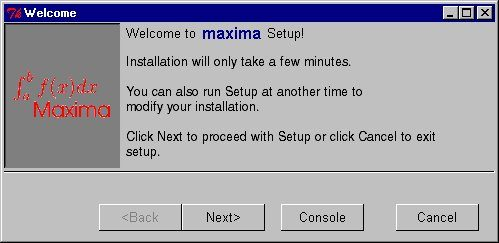
\includegraphics{images/maximawindowsinstall1}}
\vspace{0.3cm}
\begin{enumerate}
\item [3.]Simply follow the menus from that point - the install dialog
should be very clear. Do read the README and License when they are
presented - the information there is good to know.
\item [4.]Simply launch the program from it's icon - everything should work
out of box. It is known to run on the following versions of Windows:

\vspace{3ex}

Windows 98

\end{enumerate}

\subsection{The Hard Way}

Compiling on Windows (I have no idea how to do this.)


\chapter{Available Interfaces to Maxima}
  
Maxima is at heart a command line program, and by itself it is not
capable of displaying formatted mathematics beyond the ascii text
level. However there are other interfaces which may be used. Maxima
has the ability to export expressions using the \TeX{} syntax, and
several programs use this device to help with output formatting. (None
at this time allow formatted input.) All have their strengths and
weaknesses - the choice will likely depend on the skill of the user
and the task at hand. We will discuss here all of the interfaces currently
available, and the user can make the choice him/herself which one
to use. 


\section{The Terminal Interface}

~

{\centering \includegraphics{images/terminalshot} \par }

~

The terminal interface is the original interface to Maxima. While
in some sense all of the interfaces to Maxima could be termed Terminal
interfaces, when we refer to it here we mean the command line, no
frills interface you would use in an xterm or a nongraphical terminal.
It is the least capable of all the alternatives in many respects,
but it is also the least demanding. 

How comfortable this interface is depends to a large extent on what
Lisp you used to compile Maxima originally. If you used the default,
which is gcl, (what all binary packages I am aware of use) you do
not have readline support on the terminal. This means you will not
be able to use the back arrow key to go to the middle of an expression
and change it - you must erase everything as you go back. This is
a serious limitation, and if this is the case it is recommended by
the author that you either compile against a Lisp flavor such as Clisp,
which has readline support, or use one of the other interfaces. Any
of the others should solve this problem. If you choose to use this
interface, you activate it by simply typing \texttt{maxima} on the
terminal prompt. 

The only times I'd really recommend this interface are when none of
the other options are viable, such as a telnet connection from a really
primitive terminal.  The other options, especially
the Emacs mode, are far more comfortable working environments. 

\section{The Emacs Interface}

A really excellent Emacs mode has been written for Maxima, and this is probably the
choice I would recommend instead of the bare terminal, with or without
a graphical interface. You get to
go back in an expression without having to erase your expression,
and in a graphical environment you get syntax highlighting, among many other
goodies.  There is also an environment for including Maxima input in LaTeX
documents.

\subsection{Installing the Maxima Emacs Mode}

\noindent
The Emaxima package consists of the files \texttt{maxima.el},
\texttt{emaxima.el}, \texttt{maxima-symbols.el},
\texttt{maxima-font-lock.el}, \texttt{emaxima.sty} and \texttt{emaxima.lisp}.
To install, place the \texttt{.el} files, as well as
\texttt{emaxima.lisp}\footnote{If Emacs cannot find
  \texttt{emaxima.lisp}, then the \TeX{} output functions will not
  work, any attempts to get \TeX{} output will only result in standard
  output.} 
somewhere in the load path for Emacs.
Finally, if you want to run \LaTeX{} on the resulting document, put
\texttt{emaxima.sty} somewhere in the \TeX{} inputs path.  If you use
pdflatex, you'll also need \texttt{pdfcolmk.sty}.

Although AucTeX is not strictly necessary, you will most likely find it worth
you time to install it, as many of the best features of Emaxima are LaTeX
oriented.  

Copy the \texttt{.el} and \texttt{.lisp} files to the site-lisp directory of your Emacs installation.
On a Redhat Linux system, for example, this would be /usr/share/emacs/site-lisp,
/usr/local/share/emacs/site-lisp, or some variation thereof.  Copy the \texttt{.sty}
files to a directory where LaTeX can see them - I've found on Redhat Linux
/usr/share/texmf/tex/latex/base works fairly well.  Once you have done this,
run the command mktexlsr.  You should now be almost ready to roll.

The last step is to edit your .emacs file.  In order to use the enhanced terminal
mode, insert the following line:
\begin{verbatim}
(autoload 'maxima "maxima" "Maxima interaction" t)
\end{verbatim}
If you wish to associate files ending in \texttt{.max} with this particular
Emacs mode, add this line:
\begin{verbatim}
(setq auto-mode-alist (cons '("\\.max" . maxima-mode) auto-mode-alist)
\end{verbatim}
This will allow you to start Maxima from within Emacs.  You can do this
one of two ways - either start Emacs and from within it type \texttt{M-x maxima},
or from the command line type \texttt{emacs -f maxima} to have the whole thing
work in one step.  If you wish to create a desktop icon to start the command
line Maxima, simply place this line where they ask you what the name of your
program or executable is, and it should work quite smoothly.

For Maxima-mode, add the following line to .emacs:
\begin{verbatim}
(autoload 'maxima-mode "maxima" "Maxima mode" t)
\end{verbatim}
The command \texttt{M-x maxima-mode} will start you off here.

In the case of Emaxima, the line 
\begin{verbatim}
(autoload 'emaxima-mode "emaxima" "EMaxima" t)
\end{verbatim}
\noindent
should be inserted into your .emacs file.  Then typing
\texttt{M-x emaxima-mode} will start Emaxima mode.  The command 
\texttt{M-x emaxima-mark-file-as-emaxima} will put the line
\begin{verbatim}
%-*-EMaxima-*-
\end{verbatim}
\noindent
at the beginning of the file, if it isn't there already, and will ensure
that the next time the file is opened, it will be in \texttt{emaxima-mode}.  
This can be done automatically everytime a file is put in
\texttt{emaxima-mode} by putting the line
\begin{verbatim}
(add-hook 'emaxima-mode-hook 'emaxima-mark-file-as-emaxima)
\end{verbatim}
\noindent
somewhere in your \texttt{.emacs} file.

\subsection{Emaxima Mode}

Emaxima is a major mode for Emacs that allows the user to insert Maxima
sessions and code in a \LaTeX{} document.  It is based on Dan Dill's
\TeX{}/\textit{Mathematica} package\footnote{\TeX/\textit{Mathematica} is
available from \url{ftp://chem.bu.edu/pub/tex-mathematica-2.0}.}, and
uses a modified version of William Schelter's \texttt{maxima.el}.
Emaxima is an extension of the
\LaTeX{} mode provided by AUC\TeX{}\footnote{This can be configured so
that Emaxima extends the standard \TeX{} mode provided by Emacs, or just
text mode.}, and so has the \LaTeX{} mode commands available.  The
resulting document can be processed by \LaTeX{}; this requires putting 
\begin{verbatim}
\usepackage{emaxima}
\end{verbatim}
\noindent
in the preamble.

This is in no sense a graphical environment, and the user will not see
the benefits of any TeX formatting in real time.  This mode is most 
useful to those who are accustomed to writing documents in LaTeX,
and would like to include Maxima sessions in them.  This manual itself
is a good example of Emaxima in action.

\subsubsection{Cells}

The basic unit of Maxima code in Emaxima is a \textbf{cell}.  A cell
consists of text between the delimiters
\begin{verbatim}
\beginmaxima
\end{verbatim}
\noindent
and
\begin{verbatim}
\endmaxima
\end{verbatim}
\noindent
A cell can be created by typing \texttt{C-c C-o}.  (The \texttt{C-o} in this
case stands for \textbf{o}pening a cell.)  The delimiters will then be
placed in the buffer, and the point will be placed between them.

When working with several cells, you can jump between them by using
\texttt{C-c +} to go to the next cell and \texttt{C-c -} to go to the
previous cell.

\begin{figure}

\centering 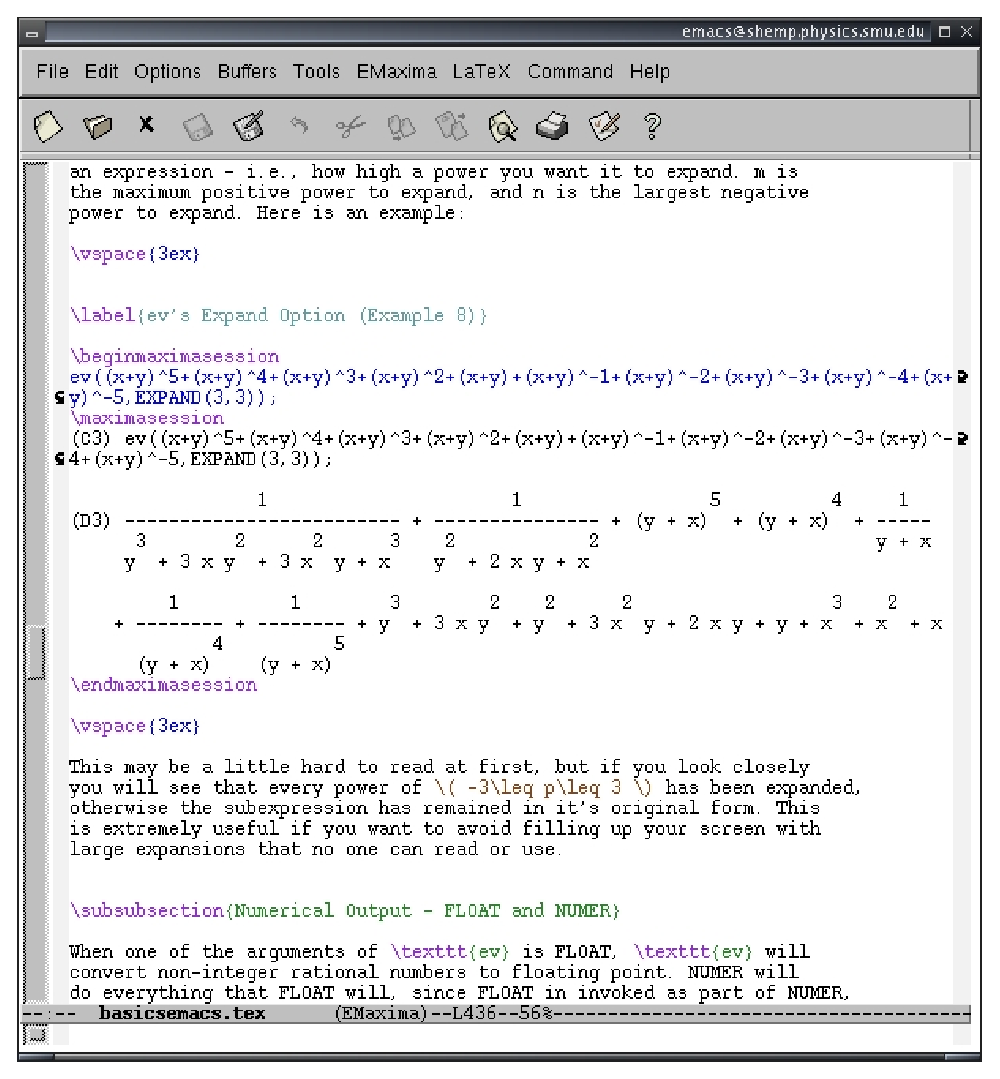
\includegraphics{images/emaximashot} \par
\caption{An Emaxima Session}

\end{figure}

\subsubsection{Evaluating cells}

\noindent
To evaluate the contents of a cell, the command
\texttt{C-cC-uc} (\texttt{emaxima-update-cell})\footnote{Sending the
  cells contents to a Maxima process and returning the results is
  called \textbf{updating} the cell, the prefix 
\texttt{C-c C-u} will be used to update cells in different ways.} 
will send the contents
of the cell to a Maxima process (if there is no Maxima process running,
one will be started) and return the results to the cell,
separated from the input by the marker
\begin{verbatim}
\maximaoutput
\end{verbatim}
\noindent
To differentiate
$sin(x^2)$, for example, type 
\texttt{diff(sin(x\^{}2),x);} in a cell:
\begin{verbatim}
\beginmaxima
diff(sin(x^2),x);
\endmaxima
\end{verbatim}
\noindent
After typing \texttt{C-c C-u c}, it will look like
\begin{verbatim}
\beginmaxima
diff(sin(x^2),x);
\maximaoutput
                                           2
                                  2 x COS(x )
\endmaxima
\end{verbatim}
\noindent
To delete the output and return the cell to its original form, you can
use the command \texttt{C-c C-d}.
If the document is to be \TeX{}ed, the above cell will look like:
\beginmaxima
diff(sin(x^2),x);
\endmaxima
and the cell with output will look like:
\beginmaxima
diff(sin(x^2),x);
\maximaoutput
                                           2
                                  2 x COS(x )
\endmaxima

Emaxima mode can take advantage of the fact that Maxima can give its
output in \LaTeX{} form.  The command \texttt{C-c C-u C}
works the same as \texttt{C-c C-u c}, except now the output is in \LaTeX{}
form, ready to be formatted by \LaTeX{}.  In general, if 
\texttt{C-c C-u }\textsl{letter} returns Maxima output, then
\texttt{C-c C-u }\textsl{capital letter} will return the output in
\TeX{} form.  The above cell would become
\begin{verbatim}
\beginmaxima
diff(sin(x^2),x);
\maximatexoutput
$$   2\*x\*\cos x^{2} $$
\endmaxima
\end{verbatim}
\noindent
which, when \LaTeX{}ed, would become
\beginmaxima
diff(sin(x^2),x);
\maximatexoutput
$$   2\*x\*\cos x^{2} $$
\endmaxima
\noindent
(Note that whenever a cell is updated, any old output is discarded and
replaced with new output.)  The command \texttt{C-c C-u a} will update all
of the cells in your document, 
stopping at each one to ask if you indeed want it updated.  Given an
argument, \texttt{C-u C-c C-u a}, it will update all of the cells in your
document without asking.  The command \texttt{C-c C-u A} behaves
similarly, except now all the output is returned in \LaTeX{}  form.

\subsubsection{Initialization Cells}

\noindent
It is possible that you want certain cells evaluated separate from the
others; perhaps, for example, you want certain cells evaluated whenever
you open the document.  This can be done using initialization cells.
An initialization cell is delimited by
\begin{verbatim}
\beginmaxima[* Initialization Cell *]
\end{verbatim}
\noindent
and
\begin{verbatim}
\endmaxima
\end{verbatim}
\noindent
The command \texttt{C-c C-t} will turn a cell into
an initialization cell, applying \texttt{C-c C-t} again will turn it
back into a regular cell.  
When \LaTeX{}ed, an initialization cell will look like
\beginmaxima[* Initialization Cell *]
diff(sin(x^2),x);
\endmaxima

Initialization cells behave like regular
cells, except that they can be treated as a group.
To evaluate all initialization cells (without displaying the output in
the document buffer), the
command \texttt{C-c C-u t} will go to each of the
initialization cells and evaluate them.
If you want the output of the initialization cells to be brought back 
to the document buffer,  stopping at each one to see it
you indeed want it updated, then use the command \texttt{C-c C-u i}.
With an argument, \texttt{C-u C-c C-u i}, the
initialization cells will be updated without asking.   The command 
\texttt{C-c C-u I} behaves just like \texttt{C-c C-u i},
except that the output is returned in \TeX{} form.

\subsubsection{Referencing Other Cells}

\noindent
Instead of Maxima code, a cell can contain a reference to another cell,
and when the original cell is sent to Maxima, the reference is replaced
by the referenced cell's contents (but only in the Maxima process
buffer, the cell's 
content in the document's buffer is not changed).  In order to do
this, the original cell must be marked by having a label of the form
\texttt{<}\textsl{filename}\texttt{:}\textsl{cell label}\texttt{>}.
(The reason for the \textsl{filename} will become apparent later, and
\textsl{cell label} is optional for the referencing cell.)
The referenced cell must also be labeled, with the same
\textsl{filename} but a unique \textsl{cell label}.  To reference the
other cell, the original cell need only contain the marker for the
referenced cell.  For example, given cell 1:
\begin{verbatim}
\beginmaxima<filename:optional>
<filename:definef>
diff(f(x),x);
\endmaxima
\end{verbatim}
\noindent
and cell 2:
\begin{verbatim}
\beginmaxima<filename:definef>
f(x):=sin(x^2);
\endmaxima
\end{verbatim}
\noindent
then the result of updating cell 1 (\texttt{C-c C-u c}) will be:
\begin{verbatim}
\beginmaxima<filename:optional>
<filename:definef>
diff(f(x),x);
\maximaoutput
                                             2
                                f(x) := SIN(x )
                                           2
                                  2 x COS(x )
\endmaxima
\end{verbatim}
\noindent
When \LaTeX{}ed, the top line will contain a copy of the marker.

\beginmaxima<filename:optional>
<filename:definef>
diff(f(x),x);
\maximaoutput
                                             2
                                f(x) := SIN(x )
                                           2
                                  2 x COS(x )
\endmaxima

A cell can contain more than one reference, and referenced cells can
themselves contain references.  

To aid in labelling the cells, the command \texttt{C-c C-x}
will prompt for a label name and label the
cell.  To aid in calling references, the command \texttt{C-c C-TAB}
can be used for completing the
the \textsl{filename} and \textsl{cell label} parts of a reference, 
based on the current labels.  
Another option is to set the Emacs variable
\texttt{emaxima-abbreviations-allowed} to \texttt{t}, say, by putting
the line
\begin{verbatim}
(setq emaxima-abbreviations-allowed t)
\end{verbatim}
\noindent
in your \texttt{.emacs} file.  This will allow the \textsl{filename}
and \textsl{cell label} parts of a reference to be abbreviated by enough
of a prefix to uniquely identify it, followed by ellipses
\texttt{...}
For example, if there are cells labelled
\begin{verbatim}
<filename:long description>
<filename:lengthy description>
\end{verbatim}
\noindent
Then the reference
\begin{verbatim}
<...:le...>
\end{verbatim}
\noindent
will suffice to refer to the second label above.

If you want the references in a cell to be replaced by the actual
code, the command \texttt{C-c @} will expand all the
references and put the code into a separate buffer (so it will not
affect the original document).

\subsubsection{WEB}

\noindent
The reason for the ability to reference other cells is so that you can
write what Donald Knuth calls literate programs.  The idea is that the
program is written in a form natural to the author rather than natural
to the computer.  (Another aspect of Knuth's system is that the code
is carefully documented, hence the name ``literate programming'', but
that is done naturally in Emaxima.)  Knuth called his original
literate programming tool \texttt{WEB}, since, as he puts it,
``the structure of a software program may be thought of as a web that
is made up of many interconnected pieces.''  
Emaxima's ability in this respect is taken directly from
\TeX{}/\textit{Mathematica}, and is ultimately based on
\texttt{WEB}. To create a 
program, the ``base cell'' or ``package cell'' should contain 
a label of the form \texttt{<}\textsl{filename}\texttt{:>} 
(no cell label), and can
contain references of the form 
\texttt{<}\textsl{filename}\texttt{:}\textsl{part}\texttt{>}
(same file name as the base cell).  

As a simple (and rather silly) example, suppose we want to create a
program to sum the first $n$ squares.  We could start:
\begin{verbatim}
\beginmaxima<squaresum.max:>
squaresum(n) := (
  <squaresum.max:makelist>
  <squaresum.max:squarelist>
  <squaresum.max:addlist>
  );        
\endmaxima
\end{verbatim}
\noindent
We would then need cells
\begin{verbatim}
\beginmaxima<squaresum.max:makelist>,
L:makelist(k,k,1,n),
\endmaxima

\beginmaxima<squaresum.max:squarelist>
<squaresum.max:definesquare>
L:map(square,L),
\endmaxima

\beginmaxima<squaresum.max:addlist>
lsum(k,k,L)
\endmaxima
\end{verbatim}
\noindent
and then we would also need:
\begin{verbatim}
\beginmaxima<squaresum.max:definesquare>
square(k) := k^2,
\endmaxima
\end{verbatim}
\noindent
When \TeX{}ed, the header of the cell will say that it determines the
file \texttt{squaresum.mu}.  
\beginmaxima<squaresum.max:>
squaresum(n) := (
  <squaresum.max:makelist>
  <squaresum.max:squarelist>
  <squaresum.max:addlist>
  );        
\endmaxima

The command 
\texttt{C-u C-c @} will put all the pieces
together in the file it determines.  The resulting file, in this case,
will be \texttt{squaresum.max} and will look like:
\begin{verbatim}
squaresum(n) := (
  L:makelist(k,k,1,n),
  square(k) := k^2,
  L:map(square,L),
  lsum(k,k,L)
  );        
\end{verbatim}
\noindent
(Although the idea is that only the computer need look at this file.)

\subsubsection{Other types of cells}

\noindent
When a cell is \TeX{}ed, the input and output are kept separate.  To
have the results look like a Maxima session, there are, in addition to
the standard cells, special cells called \emph{session cells}.   A
session cell is delimited by
\begin{verbatim}
\beginmaximasession
\end{verbatim}
\noindent
and
\begin{verbatim}
\endmaximasession
\end{verbatim}
\noindent
The command \texttt{C-c C-p} will create a session cell.  When a
session cell is updated, the output will be marked off with
\verb+\maximasession+, and will contain both the input and the output,
with the Maxima prompts.  For example, if the session cell
\begin{verbatim}
\beginmaximasession
diff(sin(x),x);
int(cos(x),x);
\endmaximasession
\end{verbatim}
\noindent
were updated, the result would look like
\begin{verbatim}
\beginmaximasession
diff(sin(x),x);
integrate(cos(x),x);
\maximasession
(C1)diff(sin(x),x);

(D1)                                COS(x)
(C2)integrate(cos(x),x);

(D2)                                SIN(x)
\endmaximasession
\end{verbatim}
\noindent
which, when \TeX{}ed, would look like
\beginmaximasession
diff(sin(x),x);
integrate(cos(x),x);
\maximasession
(C1)diff(sin(x),x);

(D1)                                COS(x)
(C2)integrate(cos(x),x);

(D2)                                SIN(x)
\endmaximasession
\noindent
If it is updated in \TeX{} form, it will look like
\begin{verbatim}
\beginmaximasession
diff(sin(x),x);
integrate(cos(x),x);
\maximatexsession
\C1.  diff(sin(x),x); \\
\D1.   \cos x \\
\C2.  integrate(cos(x),x); \\
\D2.   \sin x \\
\endmaximasession
\end{verbatim}
\noindent
which, when \TeX{}ed, will look like
\beginmaximasession
diff(sin(x),x);
integrate(cos(x),x);
\maximatexsession
\C1.  diff(sin(x),x); \\
\D1.   \cos x \\
\C2.  integrate(cos(x),x); \\
\D2.   \sin x \\
\endmaximasession

For particularly long output lines inside the \verb+\maximatexsession+
part of a session cell, the command \verb+\DD+ will typeset anything
between the command and \verb+\\+.  Unfortunately, to take advantage
of this, the output has to be broken up by hand.
If a session cell has not been updated, or has no output for some
other reason, it will not appear when the document is \TeX{}ed.

There is one other type of cell, a \emph{noshow cell}, which can be
used to send Maxima a command, but won't appear in the \TeX{}ed
output. A noshow cell can be created with \texttt{C-c C-n}, and will
be delimited by
\begin{verbatim}
\beginmaximanoshow
\end{verbatim}
\noindent
and
\begin{verbatim}
\endmaximanoshow
\end{verbatim}

Session cells and noshow cells cannot be initialization cells or part of
packages.\footnote{That could be changed, but I don't know why it'd be
useful.} 

If the command to create one type of cell is called while inside
another type of cell, the type of cell will be changed.  So, for
example, the command \texttt{C-c C-p} from inside the cell
\begin{verbatim}
\beginmaxima
diff(x*sin(x),x);
\endmaxima
\end{verbatim}
\noindent
will result in
\begin{verbatim}
\beginmaximasession
diff(x*sin(x),x);
\endmaximasession
\end{verbatim}
\noindent
If a standard cell is an initialization cell or a package part, its
type cannot be changed.


\subsubsection{Miscellaneous}

\noindent
Some Maxima commands can be used even outside of cells.  The command 
\texttt{C-c C-u l} send the current line to a
Maxima process, comment out the current line, and insert the Maxima
output in the current buffer.  The command 
\texttt{C-c C-u L} will do the same, but
return the result in \LaTeX{} form.

The command \texttt{C-c C-h} will provide
information on a prompted for function (like Maxima's \texttt{describe}), 
and  \texttt{C-c C-i} will give the Maxima info manual.

Finally, the Maxima process can be killed with \texttt{C-c C-k}.

\subsubsection{Customizing EMaxima}

\noindent
There are a few things that you can do to customize Emaxima.  

By default, Emaxima is an extension of AUC\TeX{} mode.  This can be
changed by changing the variable \texttt{emaxima-use-tex}.  The possible
values are \texttt{'auctex}, \texttt{'tex} and \texttt{nil}.  Setting
\texttt{emaxima-use-tex} (the default) to \texttt{'auctex} will make Emaxima
an extension of AUC\TeX{}, setting it to \texttt{'tex} will make Emaxima an
extension of Emacs's default \TeX{} mode, and setting
\texttt{emaxima-use-tex} to \texttt{nil} will make Emaxima an extension of
text-mode.  So, for example, putting 
\begin{verbatim}
(setq emaxima-use-tex nil)
\end{verbatim}
\noindent
in your \texttt{.emacs} file will make Emaxima default to an extension of
text mode. 

Whether or not the dots (\dots{}) abbreviation is allowed in cell
references is controlled by the elisp variable
\texttt{emaxima-abbreviations-allowed}, which is set to \texttt{t} by
default.  Setting this to \texttt{nil} will disallow the abbreviations,
but will speed up package assembly.

The \LaTeX{}ed output can also be configured in a couple of ways.
The lines that appear around cells when the document is \TeX{}ed can be
turned off with the command (in the \LaTeX{} document)
\begin{verbatim}
\maximalinesfalse
\end{verbatim}
\noindent
They can be turned back on with the command
\begin{verbatim}
\maximalinestrue
\end{verbatim}
\noindent

The fonts used to display the Maxima input and output in a cell are by
default \texttt{cmtt10}.  They can be changed, seperately, by changing the
\TeX{} values of \verb+\maximainputfont+ and \verb+\maximaoutputfont+.
So, for example, to use \texttt{cmtt12} as the input font, use the command
\begin{verbatim}
\font\maximainputfont = cmtt12
\end{verbatim}
\noindent
The spacing in the cells can be controlled by changing the \TeX{}
variables \verb+\maximainputbaselineskip+ and
\verb+\maximaoutputbaselineskip+, and so to increase the space between
the lines of the output, the command
\begin{verbatim}
\maximaoutputbaselineskip = 14pt
\end{verbatim}
\noindent
could be used.
The amount of space that appears before a cell can be changed by changing
the value of \verb+\premaximaspace+ (by default, 0pt), and that after
a cell can be changed by changing the value of \verb+\postmaximaspace+
(by default, 1.5 ex).
 
Session cells can be configured similarly.  
Lines can be placed around a Maxima session with the command
\begin{verbatim}
\maximasessionlinestrue
\end{verbatim}
\noindent
and they can be turned back off with
\begin{verbatim}
\maximasessionlinesfalse
\end{verbatim}
\noindent
The font can be changed by changing the value of
\verb+\maximasessionfont+.  The color of the prompts when the session
is in \TeX{} form is controlled by \\
\verb+\maximapromptcolor+, by
default red, the colors of the input lines and output lines are
controlled by \verb+\maximainputcolor+ and \verb+\maximaoutputcolor+,
respectively. So the command
\begin{verbatim}
\def\maximainputcolor{green}
\end{verbatim}
\noindent
would make the input in a \TeX{}ed session green.  
The session can be \TeX{}ed without the colors by using the command
\verb+\maximasessionnocolor+.
The baselineskip is
set by \verb+\maximasessionbaselineskip+ for normal session cells, and
by \verb+\maixmatexsessionbaselineskip+ for \TeX{} sessions.  The
amount of space that appears before a session cell can be changed by
changing the value of \verb+\premaximasessionspace+ (by default, 0pt),
and that after a cell can be changed by changing the value of
\verb+\postmaximasessionspace+ (by default, 1.5 ex).

\subsubsection{Emaxima mode commands}

\noindent
\begin{tabular}{p{\firstcol}p{\secondcol}}
\hline
\textbf{Key} & \textbf{Description}\\
\hline
\texttt{C-c C-o} & Create a (standard) cell.\\
\texttt{C-c C-p} & Create a session cell.\\
\texttt{C-c C-n} & Create a noshow cell.\\
\texttt{C-c +} & Go the the next cell.\\
\texttt{C-c -} & Go to the previous cell.\\
\texttt{C-c C-u a} & 
Update all of the cells.  With an argument, don't ask before updating.\\
\texttt{C-c C-u A}
& Update all of the cells in \TeX{} form. With an argument don't ask
before updating.\\
\texttt{C-c C-u t}
& Evaluate all of the initialization cells.\\
\texttt{C-c C-u i}
& Update all of the initialization cells.  With an argument, don't
ask before updating.\\
\texttt{C-c C-u I}
& Update all of the initialization cells in \TeX{} form.  With an
argument, don't ask before updating.\\
\texttt{C-c C-u s}
& Update all of the session cells in \TeX{} form.  With an
argument, don't ask before updating.\\
\texttt{C-c C-k}
& Kill the current Maxima core - this will lose all data entered
into the maxima system up until this point by other cells.
\end{tabular}

\smallskip

\noindent
\textbf{Commands only available in cells.}

\smallskip

\noindent
\begin{tabular}{p{\firstcol}p{\secondcol}}
\hline
\textbf{Key} & \textbf{Description}\\
\hline
\texttt{C-c C-v}
%& \texttt{emaxima-send-cell}
& Send the current cell to the Maxima process.\\
\texttt{C-c C-u c}
%& \texttt{emaxima-update-cell}
& Update the current cell.\\
\texttt{C-c C-u C}
%& \texttt{emaxima-tex-update-cell}
& Update the current cell in \TeX{} form.\\
\texttt{C-c C-d}
%& \texttt{emaxima-delete-output}
& Delete the output from the current cell.\\
\texttt{C-c C-t}
%& \texttt{emaxima-toggle-init}
& Toggle whether or not the current cell is an initialization cell.\\
\texttt{C-c C-x}
%& \texttt{emaxima-package-part}
& Insert a heading for the cell indicating that it's part of a
package. \\
\texttt{C-c @}
%& \texttt{emaxima-assemble}
& Assemble the references contained in the cell.  With an argument,
assemble the package that the cell defines.\\
\texttt{C-c C-\texttt{TAB}}
%& \texttt{emaxima-insert-complete-name}
& Complete a reference within a cell.
\end{tabular}

\smallskip

\noindent
\textbf{Commands only available outside of cells.}

\smallskip

\noindent
\begin{tabular}{p{\firstcol}p{\secondcol}}
\hline
\textbf{Key} & \textbf{Description}\\
\hline
\texttt{C-c C-u l}
%& \texttt{emaxima-replace-line}
& Send the current line to Maxima, and replace the line with the
Maxima output.\\
\texttt{C-c C-u L}
%& \texttt{emaxima-replace-line-with-tex}
& Send the current line to Maxima, and replace the line with the
Maxima output in \TeX{} form.
\end{tabular}

\subsubsection{AUC\TeX{} commands}

\smallskip

\noindent
\textbf{Inserting commands}

\smallskip

\noindent
\begin{tabular}{p{\firstcol}p{\secondcol}}
\hline
\textbf{Key} & \textbf{Description}\\
\hline
\texttt{C-c C-e}
& Insert an environment.\\
\texttt{C-c C-s}
& Insert a section.\\
\texttt{C-c ]}
& Close an environment.\\
\texttt{C-c C-j}
& Insert an item into a list.\\
\texttt{"}
& Smart quote.\\
\texttt{\$}
& Smart dollar sign.\\
\texttt{C-c @}
& Insert double brace.\\
\texttt{C-c C-m}
& Insert \TeX{} macro.\\
\texttt{M-TAB}
& Complete \TeX{} macro.\\
\end{tabular}

\smallskip

\noindent
\textbf{Formatting}

\smallskip

\noindent
\begin{tabular}{p{\firstcol}p{\secondcol}}
\hline
\textbf{Key} & \textbf{Description}\\
\hline
\texttt{C-c C-q C-r}
& Format region.\\
\texttt{C-c C-q C-s}
& Format section.\\
\texttt{C-c C-q C-e}
& Format environment.\\
\texttt{C-c .}
& Mark an environment.\\
\texttt{C-c *}
& Mark a section.
\end{tabular}

\smallskip

\noindent
\textbf{Commenting}

\smallskip

\noindent
\begin{tabular}{p{\firstcol}p{\secondcol}}
\hline
\textbf{Key} & \textbf{Description}\\
\hline
\texttt{C-c ;}
& Comment a region.\\
\texttt{C-u C-c ;}
& Uncomment a region.\\
\texttt{C-c \%}
& Comment a paragraph.\\
\texttt{C-u C-c \%}
& Uncomment a paragraph.
\end{tabular}

\smallskip

\noindent
\textbf{Font selection}

\smallskip

\noindent
\begin{tabular}{p{\firstcol}p{\secondcol}}
\hline
\textbf{Key} & \textbf{Description}\\
\hline
\texttt{C-c C-f C-b}
& Bold.\\
\texttt{C-c C-f C-i}
& Italics.\\
\texttt{C-c C-f C-r}
& Roman.\\
\texttt{C-c C-f C-e}
& Emphasized.\\
\texttt{C-c C-f C-t}
& Typewriter.\\
\texttt{C-c C-f C-s}
& Slanted.\\
\texttt{C-c C-f C-d}
& Delete font.\\
\texttt{C-u C-c C-f}
& Change font.
\end{tabular}

\smallskip

\noindent
\textbf{Running \TeX{}}

\smallskip

\noindent
(Commands: \texttt{TeX}, \texttt{TeX Interactive}, \texttt{LaTeX},
\texttt{LaTeX Interactive}, \texttt{SliTeX}, \texttt{View},
\texttt{Print}, \texttt{BibTeX}, \texttt{Index}, \texttt{Check},
\texttt{File}, \texttt{Spell}.)

\smallskip

\noindent
\begin{tabular}{p{\firstcol}p{\secondcol}}
\hline
\textbf{Key} & \textbf{Description}\\
\hline
\texttt{C-c C-c}
& Run a command on the master file.\\
\texttt{C-c C-r}
& Run a command on the current region.\\
\texttt{C-c C-b}
& Run a command on the buffer.\\
\texttt{C-c `}
& Go to the next error.\\
\texttt{C-c C-k}
& Kill the \TeX{} process.\\
\texttt{C-c C-l}
& Center the output buffer.\\
\texttt{C-c C-\^{}}
& Switch to the master file.\\
\texttt{C-c C-w}
& Toggle debug of overful boxes.\\
\end{tabular}

\subsection{Maxima-mode}

There is a second choice for document editing with Emacs and Maxima, which 
is not dependant on LaTeX.  That is Maxima-mode, which basically amounts
to a text editor which allows you to send lines to Maxima.  It does not
have all the abilities of Emaxima, but is somewhat more flexible than interactive
Maxima use.

For moving around in the code, Maxima mode provides the following

\noindent
Maxima mode has the following completions commands:

\textbf{Motion}

\smallskip

\noindent
\begin{tabular}{p{\firstcol}p{\secondcol}}
\hline
\textbf{Key} & \textbf{Description}\\
\hline
\texttt{M-C-a} & Go to the beginning of the form.\\
\texttt{M-C-e} & Go to the end of the form.\\
\texttt{M-C-b} & Go to the beginning of the sexp.\\
\texttt{M-C-f} & Go to the end of the sexp.
\end{tabular}

\smallskip

\noindent
\textbf{Process}

\smallskip

\noindent
\begin{tabular}{p{\firstcol}p{\secondcol}}
\hline
\textbf{Key} & \textbf{Description}\\
\hline
\texttt{C-cC-p} & Start a Maxima process.\\
\texttt{C-cC-r} & Send the region to the Maxima process.\\
\texttt{C-cC-b} & Send the buffer to the Maxima process.\\
\texttt{C-cC-c} & Send the line to the Maxima process.\\
\texttt{C-cC-e} & Send the form to the Maxima process.\\
\texttt{C-cC-k} & Kill the Maxima process.\\
\texttt{C-cC-p} & Display the Maxima buffer.
\end{tabular}

\smallskip

\noindent
\textbf{Completion}

\smallskip

\noindent
\begin{tabular}{p{\firstcol}p{\secondcol}}
\hline
\textbf{Key} & \textbf{Description}\\
\hline
\texttt{M-TAB} & Complete the Maxima symbol.\\
\texttt{C-TAB} & Cycle through completions of the Maxima symbol.\\
\end{tabular}

\smallskip

\noindent
\textbf{Comments}

\smallskip

\noindent
\begin{tabular}{p{\firstcol}p{\secondcol}}
\hline
\textbf{Key} & \textbf{Description}\\
\hline
\texttt{C-c ;} & Comment the region.\\
\texttt{C-c :} & Uncomment the region.\\
\texttt{M-;} & Insert a short comment.\\
\texttt{C-c *} & Insert a comment environment.
\end{tabular}


\smallskip

\noindent
\textbf{Indentation}

\smallskip

\noindent
\begin{tabular}{p{\firstcol}p{\secondcol}}
\hline
\textbf{Key} & \textbf{Description}\\
\hline
\texttt{TAB} & Indent line.\\
\texttt{M-C-q} & Indent form.
\end{tabular}


\smallskip

\noindent
\textbf{Maxima help}

\smallskip

\noindent
\begin{tabular}{p{\firstcol}p{\secondcol}}
\hline
\textbf{Key} & \textbf{Description}\\
\hline
\texttt{C-c C-d}
%& \texttt{maxima-help}
& Get help on a (prompted for) subject.\\
\texttt{C-c C-m}
%& \texttt{maxima-apropos}
& Read the manual.\\
\texttt{C-cC-h} & Get help with the symbol under point.\\
\texttt{C-cC-a} & Get apropos with the symbol under point.
\end{tabular}

\smallskip

\noindent
\textbf{Miscellaneous}

\smallskip

\noindent
\begin{tabular}{p{\firstcol}p{\secondcol}}
\hline
\textbf{Key} & \textbf{Description}\\
\hline
\texttt{M-C-h} & Mark the form.\\
\texttt{C-c)} & Check the region for balanced parentheses.\\
\texttt{C-c C-)} & Check the form for balanced parentheses.
\end{tabular}

\begin{figure}
\centering 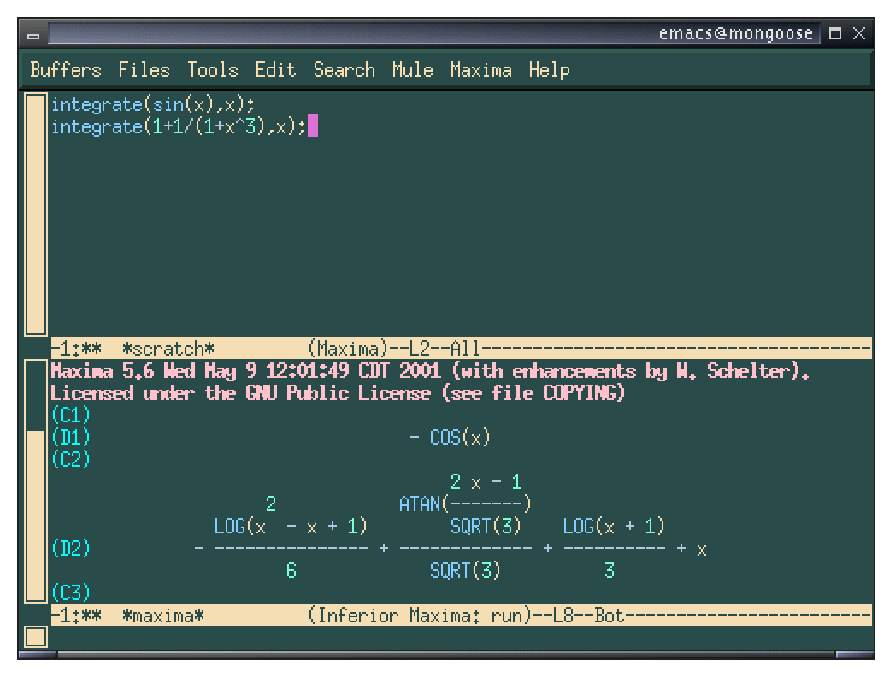
\includegraphics{images/emacsmaximamodeshot} 
\caption{Maxima-mode} 
\end{figure}

\noindent
When something is sent to Maxima, a buffer running an inferior Maxima 
process will appear.  It can also be made to appear by using the command
\texttt{C-c C-p}.
If an argument is given to a command to send information to Maxima,
the region (buffer, line, form) will first be checked to make sure
the parentheses are balanced.
The Maxima process can be killed, after asking for confirmation 
with \texttt{C-cC-k}.  To kill without confirmation, give \texttt{C-cC-k}
an argument.

By default, a newline will be indented to the same level as the 
previous line, with an additional space added for open parentheses.
A tab will add extra spaces, as determined by the value of the 
variable \texttt{maxima-indent-amount}.  By default, this is 2.
The behaviour of newline and indent can be changed by the command 
\texttt{M-x maxima-change-newline-style}.  The possibilities are:
\begin{description}
\item[Basic] A newline will have no indentation, and indentation
               must be added with tabs.
\item[Standard]      As above.
\item[Perhaps smart] Tries to guess an appropriate indentation, based on
               open parentheses, "do" loops, etc.
               A newline will re-indent the current line, then indent
               the new line an appropriate amount.
\end{description}
The default can be set by setting the value of the variable 
\texttt{maxima-newline-style} to either \texttt{'basic}, 
\texttt{'standard} or \texttt{'perhaps-smart}.
In all cases, \texttt{M-x maxima-untab} will remove a level of indentation.

\subsection{Enhanced Terminal Mode}

For those just want a better terminal session, you can run a regular terminal
style session in Emacs.  This gives you everything the 
terminal interface does, plus syntax highlighting, plus more flexibility when
editing your commands.  If you already have a copy of Emacs open, you can start
up the Maxima buffer by typing \verb@ M-x maxima @.  If you do not have Emacs
running, a shortcut is to start emacs using the following command: \verb@ emacs -f maxima @.  

\begin{figure}
\centering 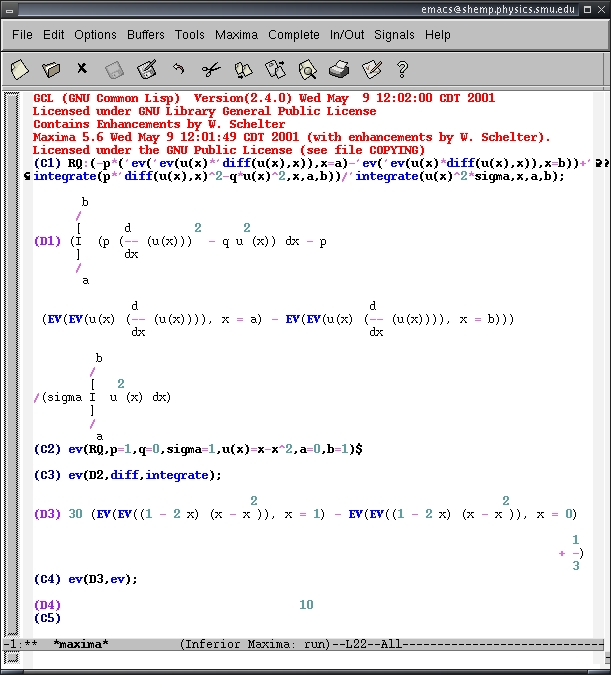
\includegraphics{images/emacsshot}
\caption{Interactive Session}
\end{figure}

In the Maxima process buffer,
return will check the line for balanced parentheses, and send line as input.
Control return will send the line as input without checking for balanced
parentheses.  The following commands are also available.

\smallskip

\begin{tabular}{p{\firstcol}p{\secondcol}}
\texttt{M-TAB} & Complete the Maxima symbol as much as possible, providing
     a completion buffer if there is more than one possible completion.\\
\texttt{C-TAB} & Cycle through possible completions.\\
\texttt{C-M-TAB} & Complete the input line, based on previous input lines.\\
\texttt{C-c C-d} & Get help on a Maxima topic.\\
\texttt{C-c C-m} & Bring up the Maxima info manual.\\
\texttt{C-cC-k} & Kill the process and the buffer, after asking for
  confirmation.  To kill without confirmation, give \texttt{C-cC-k} an
  argument.\\
\texttt{M-p} & Bring the previous input to the current prompt.\\
\texttt{M-n} & Bring the next input to the prompt.\\
\texttt{M-r} & Bring the previous input matching
  a regular expression to the prompt.\\
\texttt{M-s} & Bring the next input matching
  a regular expression to the prompt.
\end{tabular}
\section{Xmaxima}
~

{\centering 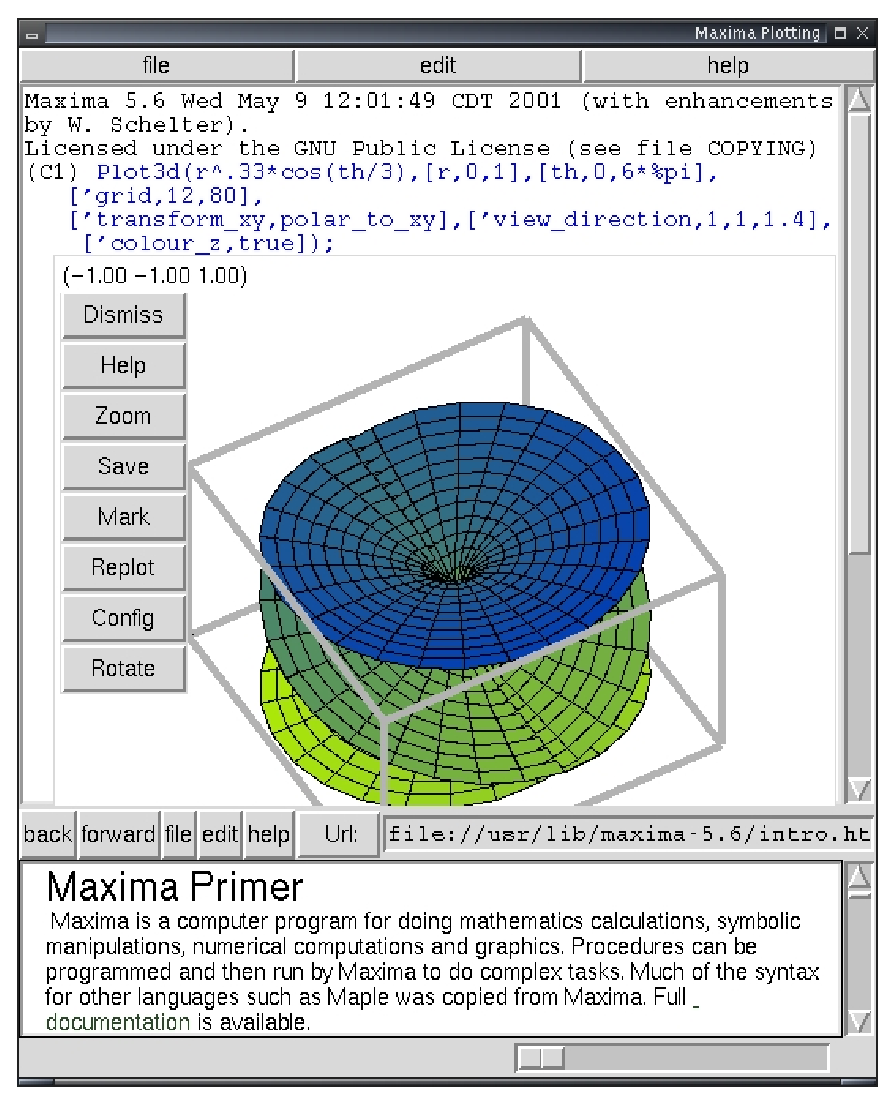
\includegraphics{images/xmaxima} \par}

~

Xmaxima is a new development in the lifetime of Maxima. It is based
on Tcl/Tk, and has the nifty feature of in-line plotting when using
the default plotting routine. No version earlier than ? has this interface,
so if you aren't using the new versions you won't have this included
in your default package. This is probably where most people will start
learning Maxima, and it is not a bad place to start. You avoid the
earlier mentioned limitations of the vanilla terminal, and avoid having
to master the setup for Emacs. In order to start this interface simply
type xmaxima in a terminal. From there, you should get what looks
like the terminal interface in a Tk window, with an introductory html
document below it. There is also a pull down menu system. For Windows
users, this will more than likely be the default choice. Symaxx and
\TeX{}macs are Unix only.

\section{Symaxx}

In the words of its creator Markus Nentwig ``Symaxx provides those 5\% of features,
that are needed to do 95\% of your work.'' Perhaps the best description
of its display is that of a mathematical flowchart - it indicates relationships
between cells with arrows, and allows free placement of expressions on a
canvas.  It is more graphical than
any of the other Maxima interfaces, and although input is still ascii
based the output is formatted. It is based on Perl and Tk, both of
which are required to run it. This interface tends, at least in the
experience of this author, to be a bit resource intensive, but allows
some page formatting possibilities which make it a very interesting
program. We will show you some of its features here, and if you decide to use
this interfacethe Symaxx manual is a highly recommended
read.

~

{\centering 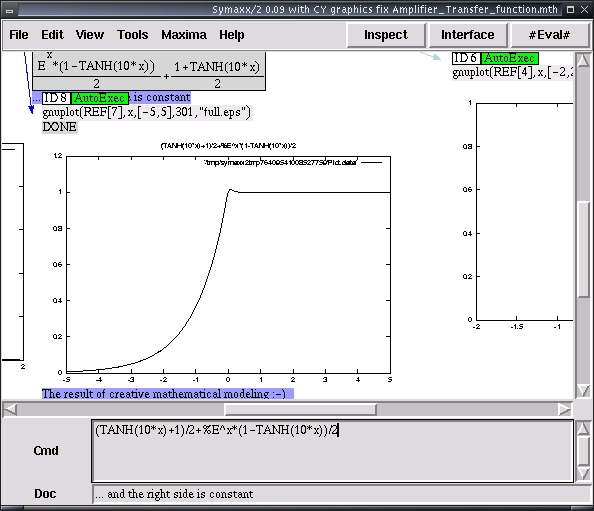
\includegraphics{images/symaxx} \par}

~
 
Symaxx uses a fairly basic display format - each unit of mathematical input
and output is labeled with an ID number, which one can use to refer to 
that particular unit elsewhere in your document.  There are three levels to
each unit - the input box, which displays the command input into Maxima,
the output box, which displays the results, and the documentation box,
where you can record information and descriptions which are not intended
to be evaluated.  This may take a little getting used to - pressing return
once you are done creating the input expression doesn't evaluate it, but only
sends it to the formatter used by Symaxx to create a graphical representation
of the input.  To send the command to Maxima, you press the evaluate button.

For graphing purposes, Symaxx is able to embed gnuplot figures.  Also included
in its abilities are the ability to use TeX to display output, manipulate
units, and export to postscript files.  Here is a sample output showing
these abilities in action:

~

{\centering 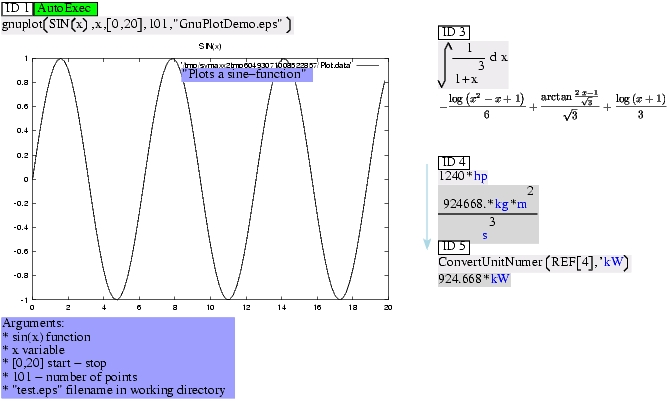
\includegraphics{images/symaxxoutput} \par}

~

(Add to
troubleshooting tips:  Some versions
of Symaxx seem to have trouble interacting with some versions of netpbm - if Symaxx
should fail to display graphs, try this solution:
~
get solution from Symaxx discussion forum
~
)

In order to utilize the full abilities of Symaxx, you must have a fair bit of
supporting software installed.  There is Maxima itself, of course, and then there
are the following:
\begin{itemize}
\item Perl
\item Tk800.022
\item netpbm
\item \TeX{} for advanced output formatting 
\end{itemize}

Here are some basic install instructions. We will assume here you need to install
Tk800.022 and Symaxx, having already installed the others earlier.  If you haven't
they are readily available on most Linux distributions.

\begin{verbatim}
user$ tar -xvzf Tk800.022.tar.gz 
user$ cd Tk800.022

If you have root access, do the following:

user$ perl Makefile.PL
user$ make
user$ make test (optional)
user$ su
Password:
root$ make install

if you don't have root access, use

user$ perl Makefile.PL LIB=/home/(place to install) or
user$ perl Makefile.PL PREFIX=/home/(place to install).
user$ make; make install
\end{verbatim}

Find the location of the folder `Tk' in the folder you gave as argument to LIB or
PREFIX. Now you'll have to change the first line in `symaxx' and `Symaxx2/Watchdog'
to include the Tk library. Append a
\verb@-I /home/(where you installed Tk)/@ \verb@(The folder that contains Tk)@
as in
\verb@ #!/usr/bin/perl -w -I /home/somewhere/ @

Then simply decompress Symaxx in the directory of your choice. If perl is not in /usr/bin, you'll have to change the first line of the files `symaxx'
and `Symaxx2/Watchdog' to the location on your system, as found by `whereis
perl'.

\section{\TeX{}macs}

\TeX{}macs is a new WYSIWYG scientific editor, and it has the ability
to interface with many computer algebra systems, including Maxima.
This program takes advantage of the \TeX{} output Maxima can produce
to format it's output. To launch Maxima inside of \TeX{}macs you go
up to the menu and select Insert -> sessions -> maxima. Then things
work like they do in xmaxima or Emacs. This is probably the most visually
appealing way to run Maxima.

~

{\centering 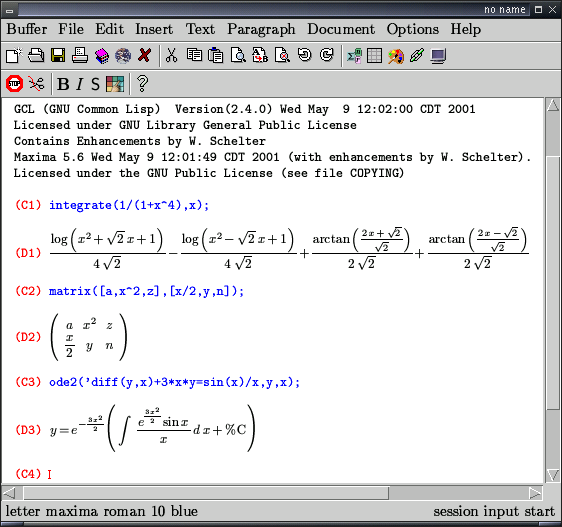
\includegraphics{images/texmacs} \par }


\chapter{The Basics - What you need to know to operate in Maxima}
  %-*-EMaxima-*-

Here we will attempt to address universal concepts which you will 
need to know when using Maxima for a wide variety of tasks. 


\section{The Very Beginning}

All computer algebra systems have syntactical rules, i.e. a structured
language by which the user communicates his/her commands to the system.
Without being able to communicate in this language, it is impossible
to accomplish anything in such as system. So we will attempt to describe
herein the basics.


\subsection{Our first Maxima Session}

We will start by demonstrating the ultimate basics: \( + \), \( - \),
\( * \), and /. These symbols are virtually universal in any mathematical
system, and mean exactly what you think they mean. We will demonstrate
this, and at the same time introduce you to your first session in
Maxima. In the interface of your choice, try the following:

\vspace{3ex}

\texttt{\label{Example1}GCL (GNU Common Lisp)~ Version(2.3.8) Wed
Sep~ 5 08:00:22 CDT 2001}

\texttt{Licensed under GNU Library General Public License}

\texttt{Contains Enhancements by W. Schelter}

\texttt{Maxima 5.5 Wed Sep 5 07:59:43 CDT 2001 (with enhancements
by W. Schelter).}

\texttt{Licensed under the GNU Public License (see file COPYING)}

\beginmaximasession
2+2;
3-1;
3*4;
9/3;
9/4;
quit();
\maximatexsession
\C1.  2+2; \\
\D1.   4 \\
\C2.  3-1; \\
\D2.   2 \\
\C3.  3*4; \\
\D3.   12 \\
\C4.  9/3; \\
\D4.   3 \\
\C5.  9/4; \\
\D5.   {{9}\over{4}} \\
\C6.  quit(); \\
\endmaximasession

\vspace{3ex}

Above is our first example of a Maxima session. We notice already
several characteristics of a Maxima session: The startup message,
which gives the version of Maxima being used, the date of compilation, 
which is the day your executable was created, the labels in front of
each line, the semicolon at the end of each line, and the way we exit
the session. The startup message is not important to the session,
but you should take note of what version of Maxima you are using,
especially if there is a known problem in an earlier version which
might impact what you are trying to do. 


\subsubsection{Exiting\index{Exiting} \index{Quitting}\index{Debugging!Exiting}a
Maxima Session}

You want to be able to get out of what you get into. So the first
command we discuss will be the command that gets you out of Maxima,
and while we are at it we will discuss how to get out of debugging
mode. Debugging mode is quite useful for some things, and the reader
is encouraged to look to later chapters for an in-depth look at the
debugging mode, but for now we will stick to basics. As you see above,
\texttt{quit();} is the command which will exit Maxima. This is a
bit confusing for new users, but you must type that full command.
Simply typing \texttt{quit} or \texttt{exit} will not work, nor will
pressing \texttt{CTRL-C} - if you try the latter you will be dumped
into the debugging mode. If that happens, simply type \texttt{:q}
if you are running GNU Common Lisp, or \texttt{:a} if running CLISP.
(If in doubt use \texttt{:q} - most binary packages use GCL at this
time.) Here's an example of what not to do, and how to get out of
it if you do:

\vspace{3ex}

\texttt{\label{Quitting Maxima (Example 2)}(C1) quit;}

\texttt{~}

\texttt{(D1)~~~~~~~~~~~~~~~~~~~~~~~~~~~~~~~~
QUIT}

\texttt{(C2) exit;}

\texttt{~}

\texttt{(D2)~~~~~~~~~~~~~~~~~~~~~~~~~~~~~~~~
EXIT}

\texttt{(C3) }

\texttt{Correctable error: Console interrupt.}

\texttt{Signalled by MACSYMA-TOP-LEVEL.}

\texttt{If continued: Type :r to resume execution, or :q to quit to
top level.}

\texttt{Broken at SYSTEM:TERMINAL-INTERRUPT.~ Type :H for Help.}

\texttt{MAXIMA>\,{}>}

\texttt{Correctable error: Console interrupt.}

\texttt{Signalled by SYSTEM:UNIVERSAL-ERROR-HANDLER.}

\texttt{If continued: Type :r to resume execution, or :q to quit to
top level.}

\texttt{Broken at SYSTEM:TERMINAL-INTERRUPT.}

\texttt{MAXIMA>\,{}>\,{}>:q}

\texttt{~}

\texttt{(C3) quit()};

\vspace{3ex}

The first two lines show what happens if you forget the \texttt{()}
or type \texttt{exit}. Nothing major, but you won't exit Maxima. \texttt{CTRL-C}
causes a few more problems - if you actually read the message, you
will see it tells you how to handle it. In the above example, \texttt{CTRL-C}
was hit twice - that is not a proper way to exit Maxima either. Just
remember to use \texttt{:q} to exit debugging and \texttt{quit();}
to exit Maxima, and you should always be able to escape trouble.  If you find
youself trying to read a long output going by quickly on a terminal, press 
\texttt{CTRL-S} to temporarily halt the output, and \texttt{CTRL-Q} to resume.


\subsubsection{The End of Entry Character}

All expressions entered into Maxima must end with either the ; character
or the \$ character. The ; character is the standard character to
use for this purpose. \index{Hiding output}The \$ symbol, while performing
the same job of ending the line, suppresses the output of that line.
This example illustrates these properties:

\vspace{3ex}

\label{End of Entry Characters (Example 3)}

\beginmaximasession
x^5+3*x^4+2*x^3+5*x^2+4*x+7;
x^5+3*x^4+2*x^3+5*x^2+4*x+7$
D2;
x^5+3*x^4+2*x^3
+5*x^2+4*x+7;
x^5+3*x^4+2*x^3
     +5*x^2+4*x+7;
\maximatexsession
\C1.  x^5+3*x^4+2*x^3+5*x^2+4*x+7; \\
\D1.   x^{5}+3\*x^{4}+2\*x^{3}+5\*x^{2}+4\*x+7 \\
\C2.  x^5+3*x^4+2*x^3+5*x^2+4*x+7$ \\
\p   \\
\C3.  D2; \\
\D3.   x^{5}+3\*x^{4}+2\*x^{3}+5\*x^{2}+4\*x+7 \\
\C4.  x^5+3*x^4+2*x^3
+5*x^2+4*x+7; \\
\D4.   x^{5}+3\*x^{4}+2\*x^{3}+5\*x^{2}+4\*x+7 \\
\C5.  x^5+3*x^4+2*x^3
     +5*x^2+4*x+7; \\
\D5.   x^{5}+3\*x^{4}+2\*x^{3}+5\*x^{2}+4\*x+7 \\
\endmaximasession

\vspace{3ex}

In (C1), we input the expression using the ; character to end the
expression, and on the return line we see that D1 now contains that
expression. In (C2), we input an identical expression, except that
we use the \$ to end the line. (D2) is assigned the contents of (C2),
but does not visually display those contents. Just to verify that
(D2) does in fact contain what we think it contains we ask Maxima
to display it's contents on (C3) and we see that the are in fact present.
This is extremely useful if you are working on a problem which has
many steps, and some of those steps would produce long outputs you
don't need to actually see. In (C4), we input part of the expression,
press return, finish the expression, and then use the ; character.
Notice that the input did not end until we used that character and
pressed return - return by itself does nothing. You see (D4) contains
the same expression as (D1) shown above. To Maxima, the inputs are
the same. This can be useful if you are going to input a long expression
and wish to keep it straight visually, to avoid errors. You can also
input spaces without adversely affecting the formula, as shown in
(C5).


\subsubsection{The (C{*}) and (D{*}) Labels}

These labels are more than just line markers - they are actually the
names in memory of the contents of the lines. This is quite useful
for a number of tasks. Let's say you wish to apply a routine, say
a \texttt{solve} routine, to an expression for several different values.
Rather than retyping the entire expression, we can use the fact that
the line numbers act as markers to shorten our task considerably,
as in this example:

\vspace{3ex}

\label{Line Labels (Example 4)}

\beginmaximasession
3*x^2+7*x+5;
solve(D1=3,x);
solve(D1=7,x);
solve(D1=a,x);
\maximatexsession
\C1.  3*x^2+7*x+5; \\
\D1.   3\*x^{2}+7\*x+5 \\
\C2.  solve(D1=3,x); \\
\D2.   \left[ x=-{{1}\over{3}},\linebreak[0]x=-2 \right]  \\
\C3.  solve(D1=7,x); \\
\D3.   \left[ x=-{{\sqrt{73}+7}\over{6}},\linebreak[0]x={{\sqrt{73}-7
 }\over{6}} \right]  \\
\C4.  solve(D1=a,x); \\
\D4.   \left[ x=-{{\sqrt{12\*a-11}+7}\over{6}},\linebreak[0]x={{\sqrt{
 12\*a-11}-7}\over{6}} \right]  \\
\endmaximasession

\vspace{3ex}

In this example, we desire to solve the expression \( 3x^{2}+7x+5 \)
for \( x \) when \( 3x^{2}+7x+5=3 \), \( 3x^{2}+7x+5=7 \), and
\( 3x^{2}+7x+5=a \). (\( a \) in this case is an arbitrary constant.)
Rather than retype the equation many times, we merely enter it once,
and then use that label to set up the similar problems more easily.

\subsubsection{The (E{*}) Labels}

In some cases, particularly when a command needs to assign generated values
to variable names, the E labels will be used.  These may be treated like any
other maxima variable.  Here is an example of E label use:

\subsubsection{Custom Labels}

You do not need to settle for this method of labeling - you can define
your own expressions if you so choose, by using the : assign operator.
Let us say, for example, that we wish to solve the problem above,
but would rather call our equation FirstEquation than D1. We will
show that process here, with one deliberate error for illustration
of a property:

\vspace{3ex}

\label{Labeling an Equation (Example 5)}

\beginmaximasession
FirstEquation:3*x^2+7*x+5;
solve(FirstEquation=3,x);
solve(FirstEquation=7,x);
solve(FirstEquation=a,x);
solve(firstequation=a,x);
\maximatexsession
\C5.  FirstEquation:3*x^2+7*x+5; \\
\D5.   3\*x^{2}+7\*x+5 \\
\C6.  solve(FirstEquation=3,x); \\
\D6.   \left[ x=-{{1}\over{3}},\linebreak[0]x=-2 \right]  \\
\C7.  solve(FirstEquation=7,x); \\
\D7.   \left[ x=-{{\sqrt{73}+7}\over{6}},\linebreak[0]x={{\sqrt{73}-7
 }\over{6}} \right]  \\
\C8.  solve(FirstEquation=a,x); \\
\D8.   \left[ x=-{{\sqrt{12\*a-11}+7}\over{6}},\linebreak[0]x={{\sqrt{
 12\*a-11}-7}\over{6}} \right]  \\
\C9.  solve(firstequation=a,x); \\
\D9.   \left[  \right]  \\
\endmaximasession

\vspace{3ex}

You see that this process works exactly the same as before. On line
(C5), you see we entered the name of FirstEquation as lower case,
and the calculation failed. These names are case sensitive. This is
true of all variables. Later on you will see cases in Maxima such
as sin, where SIN and sin are the same, but it is not safe to assume
this is always true and when in doubt, watch your cases. In general 
we suggest you use lower case for your maxima commands and programs - 
it will make them easier to read and debug.


\subsection{To Evaluate or Not to Evaluate}

Operators in Maxima, such as diff for derivative, are a common feature
in many Maxima expressions. The problem is, while you need to include
an operator at a given point in your process, you may not want to
deal with the output from it at that point in the problem. Therefore,
Maxima provides the ' toggle for operators. See the example below
for an example of how this works.

\vspace{3ex}

\label{Evaluation Toggle (Example 6)}

\beginmaximasession
diff(1/sqrt(1+x^3),x);
'diff(1/sqrt(1+x^3),x);
\maximatexsession
\C10.  diff(1/sqrt(1+x^3),x); \\
\D10.   -{{3\*x^{2}}\over{2\*\left(x^{3}+1\right)^{{{3}\over{2}}}}} \\
\C11.  'diff(1/sqrt(1+x^3),x); \\
\D11.   {{d}\over{d\*x}}\*{{1}\over{\sqrt{x^{3}+1}}} \\
\endmaximasession

\vspace{3ex}

\subsection{The Concept of Environment - The \texttt{ev} Command}

All mathematical operations in Maxima take place in an environment,
which is to say the system is assuming it should do some things and
not do other things. There will be many times you will want to change
this behavior, without doing so on a global scale. Maxima provides
a way to define a local environment on a per command basis, using
the \texttt{ev} command. \texttt{ev} is one of the most powerful commands
in Maxima, and the user will benefit greatly if they master this command
early on while using Maxima. 


\subsubsection{From the top}

We will begin with a very simple example:

\vspace{3ex}

\label{Basic Use of ev Command (Example 7)}

\beginmaximasession
ev(solve(a*x^2+b*x+c=d,x),a=3,b=4,c=5,d=6);
a;
\maximatexsession
\C1.  ev(solve(a*x^2+b*x+c=d,x),a=3,b=4,c=5,d=6); \\
\D1.   \left[ x=-{{\sqrt{7}+2}\over{3}},\linebreak[0]x={{\sqrt{7}-2
 }\over{3}} \right]  \\
\C2.  a; \\
\D2.   a \\
\endmaximasession

\vspace{3ex}

The first line uses the ev command to solve for \( x \) without setting
variables in the global environment. To make sure that our variables
remain undefined, we check that \( a \) is still undefined in line
(C2), and it is.

Now lets examine some of the more interesting features of ev. The
general syntax of the ev command is ev(exp, arg1, ..., argn). exp is
an expression, like the one in the example above. You can also use
a D{*} entry name or your own name for an expression. arg{*} has many
possibilities, and we will try to step through them here.


\subsubsection{EXPAND(m,n)}

Expand is an argument which allows you to limit how Maxima expands
an expression - i.e., how high a power you want it to expand. m is
the maximum positive power to expand, and n is the largest negative
power to expand. Here is an example:

\vspace{3ex}


\label{ev's Expand Option (Example 8)}

\beginmaximasession
ev((x+y)^5+(x+y)^4+(x+y)^3+(x+y)^2+(x+y)+(x+y)^-1+(x+y)^-2+(x+y)^-3+(x+y)^-4+(x+y)^-5,EXPAND(3,3));
\maximasession
(C3) ev((x+y)^5+(x+y)^4+(x+y)^3+(x+y)^2+(x+y)+(x+y)^-1+(x+y)^-2+(x+y)^-3+(x+y)^-4+(x+y)^-5,EXPAND(3,3));

                 1                      1                 5          4     1
(D3) ------------------------- + --------------- + (y + x)  + (y + x)  + -----
      3        2      2      3    2            2                         y + x
     y  + 3 x y  + 3 x  y + x    y  + 2 x y + x

         1          1        3        2    2      2                  3    2
    + -------- + -------- + y  + 3 x y  + y  + 3 x  y + 2 x y + y + x  + x  + x
             4          5
      (y + x)    (y + x)
\endmaximasession

\vspace{3ex}

This may be a little hard to read at first, but if you look closely
you will see that every power of \( -3\leq p\leq 3 \) has been expanded,
otherwise the subexpression has remained in it's original form. This
is extremely useful if you want to avoid filling up your screen with
large expansions that no one can read or use.


\subsubsection{Numerical Output - FLOAT and NUMER}

When one of the arguments of \texttt{ev} is FLOAT, \texttt{ev} will
convert non-integer rational numbers to floating point. NUMER will
do everything that FLOAT will, since FLOAT in invoked as part of NUMER.
NUMER also handles variables defined by the user with the NUMERVAL command,
which the FLOAT toggle will leave unevaluated.  In order to evaluate these
expressions, you can also use the \texttt{float} command.

\vspace{3ex}

\label{FLOAT/NUMER example (Example 9)}

\beginmaximasession
a:9/4;
exp(a);
ev(exp(a),FLOAT);
ev(exp(a*x),FLOAT);
numerval(b, 25);
a*b;
ev(a*b,FLOAT);
ev(a*b,NUMER);
float(a);
float(b);
float(a*b);
\maximatexsession
\C1.  a:9/4; \\
\D1.   {{9}\over{4}} \\
\C2.  exp(a); \\
\D2.   e^{{{9}\over{4}}} \\
\C3.  ev(exp(a),FLOAT); \\
\D3.   9.487735836358526 \\
\C4.  ev(exp(a*x),FLOAT); \\
\D4.   e^{2.25\*x} \\
\C5.  numerval(b, 25); \\
\D5.   \left[ b \right]  \\
\C6.  a*b; \\
\D6.   {{9\*b}\over{4}} \\
\C7.  ev(a*b,FLOAT); \\
\D7.   2.25\*b \\
\C8.  ev(a*b,NUMER); \\
\D8.   56.25 \\
\C9.  float(a); \\
\D9.   2.25 \\
\C10.  float(b); \\
\D10.   25 \\
\C11.  float(a*b); \\
\D11.   56.25 \\
\endmaximasession

\vspace{3ex}

\subsubsection{Specifying Local Values for Variables, Functions, etc.}

One of the best things about the ev command is that for one evaluation
you may specify in an arg what values are to be used for the evaluation
in place of variables, how to define functions, which functions to
evaluate, etc. We will work through a series of examples here, probably
this will be the best way to illustrate the various possibilities
of this aspect of ev.

\vspace{3ex}

\beginmaximasession
eqn1:'diff(x/(x+y)+y/(y+z)+z/(z+x),x);
ev(eqn1,diff);
ev(eqn1,y=x+z);
ev(eqn1,y=x+z,diff);
\maximatexsession
\C8.  eqn1:'diff(x/(x+y)+y/(y+z)+z/(z+x),x); \\
\D8.   {{d}\over{d\*x}}\*\left({{y}\over{z+y}}+{{z}\over{z+x}}+{{x
 }\over{y+x}}\right) \\
\C9.  ev(eqn1,diff); \\
\D9.   -{{z}\over{\left(z+x\right)^{2}}}+{{1}\over{y+x}}-{{x}\over{
 \left(y+x\right)^{2}}} \\
\C10.  ev(eqn1,y=x+z); \\
\D10.   {{d}\over{d\*x}}\*\left({{z+x}\over{2\*z+x}}+{{x}\over{z+2\*x}}
 +{{z}\over{z+x}}\right) \\
\C11.  ev(eqn1,y=x+z,diff); \\
\D11.   {{1}\over{2\*z+x}}-{{z+x}\over{\left(2\*z+x\right)^{2}}}+{{1
 }\over{z+2\*x}}-{{2\*x}\over{\left(z+2\*x\right)^{2}}}-{{z}\over{
 \left(z+x\right)^{2}}} \\
\endmaximasession

\vspace{3ex}

In this example, we define eqn1 to be the derivative of a function,
but use the ' character in front of the diff operator to notify Maxima
that we don't want it to evaluate that derivative at this time. (More
on that in the ?? section.) In the next line, we use the ev with the
diff argument, which instructs ev to take all derivatives in this
expression. Now, let's say we want to define \( y \) as a function
of \( z \) and \( x \), but again avoid evaluating the derivative.
We supply our definition of \( y \) as an argument to ev, and in
(D3) we see that the substitution has been made. Now, let's evaluate
the derivative after the substitution has been made. We work as before,
except this time we supply both the new definition of \( y \) and
the diff argument, telling ev to make the substitution and then take
the derivative. In this particular case, the order of the arguments
does not matter. The case where it will matter is if you are making
multiple substitutions - then they are handled in sequence from left
to right. 

\vspace{3ex}

(need example here, one where the difference is noticeable).

\vspace{3ex}

We can also locally define functions:

\vspace{3ex}

\beginmaximasession
eqn4:f(x,y)*'diff(g(x,y),x);
ev(eqn4,f(x,y)=x+y,g(x,y)=x^2+y^2);
ev(eqn4,f(x,y)=x+y,g(x,y)=x^2+y^2,DIFF);
\maximatexsession
\C12.  eqn4:f(x,y)*'diff(g(x,y),x); \\
\D12.   f\left(x,\linebreak[0]y\right)\*\left({{d}\over{d\*x}}\*g\left(
 x,\linebreak[0]y\right)\right) \\
\C13.  ev(eqn4,f(x,y)=x+y,g(x,y)=x^2+y^2); \\
\D13.   \left(y+x\right)\*\left({{d}\over{d\*x}}\*\left(y^{2}+x^{2}
 \right)\right) \\
\C14.  ev(eqn4,f(x,y)=x+y,g(x,y)=x^2+y^2,DIFF); \\
\D14.   2\*x\*\left(y+x\right) \\
\endmaximasession

\vspace{3ex}

(At the moment, ev seems to take only the first argument in the following
example from solve: the manual seems to indicate it should be taking
both as a list??)

\vspace{3ex}

\beginmaximasession
eqn1:f(x,y)*'diff(g(x,y),x);
eqn2:3*y^2+5*y+7;
ev(eqn1,g(x,y)=x^2+y^2,f(x,y)=5*x+y^3,solve(eqn2=5,y));
ev(eqn1,g(x,y)=x^2+y^2,f(x,y)=5*x+y^3,solve(eqn2=1,y),diff);
ev(eqn1,g(x,y)=x^2+y^2,f(x,y)=5*x+y^3,solve(eqn2=1,y),diff,FLOAT);
\maximatexsession
\C15.  eqn1:f(x,y)*'diff(g(x,y),x); \\
\D15.   f\left(x,\linebreak[0]y\right)\*\left({{d}\over{d\*x}}\*g\left(
 x,\linebreak[0]y\right)\right) \\
\C16.  eqn2:3*y^2+5*y+7; \\
\D16.   3\*y^{2}+5\*y+7 \\
\C17.  ev(eqn1,g(x,y)=x^2+y^2,f(x,y)=5*x+y^3,solve(eqn2=5,y)); \\
\D17.   \left(5\*x-{{8}\over{27}}\right)\*\left({{d}\over{d\*x}}\*
 \left(x^{2}+{{4}\over{9}}\right)\right) \\
\C18.  ev(eqn1,g(x,y)=x^2+y^2,f(x,y)=5*x+y^3,solve(eqn2=1,y),diff); \\
\D18.   2\*x\*\left(5\*x-{{\left(\sqrt{47}\*i+5\right)^{3}}\over{216}}
 \right) \\
\C19.  ev(eqn1,g(x,y)=x^2+y^2,f(x,y)=5*x+y^3,solve(eqn2=1,y),diff,FLOAT); \\
\D19.   2\*x\*\left(5\*x-0.00462962962963\*\left(\sqrt{47}\*i+5\right)
 ^{3}\right) \\
\endmaximasession

\vspace{3ex}

\subsubsection{Other arguments for ev}

INFEVAL - This option leads to an "infinite evaluation" mode, where ev 
repeatedly evaluates an expression until it stops changing. To prevent a
variable, say X, from being evaluated a way in this mode, simply include 
X='X as an argument to ev. There are dangers with this command - it is 
quite possible to generate infinite evaluation loops. For example, 
ev(X,X=X+1,INFEVAL); will generate such a loop. Here is an example: (need
example where this is useful.)

\subsubsection{How ev works}

The flow of the ev command works like this:
\begin{enumerate}
\item The environment is set up by scanning the arguments.  During this 
step, a list is made of non-subscripted variables appearing on the left 
side of equations in the arguments or in the value of some arguments if 
the value is an equation.  Both subscripted variables which do not have 
associated array functions and non-subscripted variables in the 
expression exp are replaced by their global values, except for those 
appearing in the generated list.
\item If any substitutions are indicated, they are carried out.
\item The resulting expression is then re-evaluated, unless one of the 
      arguments was NO-EVAL, and simplified according to the arguments.  
      Note that any function calls in exp will be carried out AFTER the 
      variables in it are evaluated.
\item If one of the arguments was EVAL, the previous two steps are repeated.
\end{enumerate}

\subsection{Clearing values from the system - the \texttt{kill} command}

Many times you will define something in Maxima, only to want to remove 
that definition later in the computation.  The way you do this in Maxima 
is quite simple - using the \texttt{kill} command.  Here is an example:

\beginmaximasession
A:7$
A;
kill(A);
A;
\maximatexsession
\C5.  A:7$ \\
\C6.  A; \\
\D6.   7 \\
\C7.  kill(A); \\
\D7.   \mathrm{DONE} \\
\C8.  A; \\
\D8.   A \\
\endmaximasession

\texttt{kill} is used in many situations, and has many uses.  You will 
see it appear throughout this manual, in different contexts.  There are
general arguements you can use, such as \texttt{kill(all)}, which will 
essentially start you out in a new, clean environment. (Add any relevant 
general kill options here - save kill(rules) for rules section, etc.)

\section{Common Operators in Maxima}

An operator is simply something that signals a specific operation is 
to be performed. There are many, many possible operators in Maxima.  
We will address various operators for specific jobs all throughout this 
manual - this section is not comprehensive.  

\subsection{Assignment Operators}

In mathematics, we quite often want to declare functions, assign values to 
numbers, and do many similarly useful things.  Maxima has a variety of 
operators for this purpose.

\begin{enumerate}
\item [\bf{:}] The basic assignment operator.  We have already seen this 
operator in action; it is one of the most common in maxima.
\end{enumerate}

\vspace{3ex}

\beginmaximasession
A:7;
A;
\maximatexsession
\C20.  A:7; \\
\D20.   7 \\
\C21.  A; \\
\D21.   7 \\
\endmaximasession

\vspace{3ex}

\begin{enumerate}
\item [\bf{:=}] This is the operator you would use to define functions. 
 This is a common thing to do in computer algebra, so we will illustrate
both how to and how not to do this.  
\end{enumerate}

\vspace{2ex}

The right way:

\beginmaximasession
y(x):=x^2;
y(2);
\maximatexsession
\C2.  y(x):=x^2; \\
\D2.   y\left(x\right):=x^{2} \\
\C3.  y(2); \\
\D3.   4 \\
\endmaximasession

\vspace{2ex}

Several possible wrong ways:

\beginmaximasession
y:=x^2;
y=x^2;
y(2);
y(x)=x^2;
y(2);
y[x]=x^2;
y[2];
\maximatexsession
\C22.  y:=x^2; \\
\p  Improper function definition:
y
 -- an error.  Quitting.  To debug this try DEBUGMODE(TRUE);) \\
\C23.  y=x^2; \\
\D23.   y=x^{2} \\
\C24.  y(2); \\
\D24.   y\left(2\right) \\
\C25.  y(x)=x^2; \\
\D25.   y\left(x\right)=x^{2} \\
\C26.  y(2); \\
\D26.   y\left(2\right) \\
\C27.  y[x]=x^2; \\
\D27.   y_{x}=x^{2} \\
\C28.  y[2]; \\
\D28.   y_{2} \\
\C29.  y(x):=x^2; \\
\D29.   y\left(x\right):=x^{2} \\
\C30.  y(2); \\
\D30.   4 \\
\endmaximasession

\vspace{3ex}

\begin{enumerate}
\item [~] Look over the above example - it pays to
know what doesn't work.  If you recognize the error or incorrect
result you get, it will make for faster debugging.  
\end{enumerate}

\begin{enumerate}
\item [\bf{::}] This operator is related to the : operator, but does 
not function in quite the same way.  This is more what a programmer 
would refer to as a pointer.  The best way to explain is to give you 
an example of how it behaves:
\end{enumerate}

\vspace{3ex}

\beginmaximasession
A:3$
B:5;
C:'A;
C::B;
C;
A;
\maximatexsession
\C9.  A:3$ \\
\C10.  B:5; \\
\D10.   5 \\
\C11.  C:'A; \\
\D11.   A \\
\C12.  C::B; \\
\D12.   5 \\
\C13.  C; \\
\D13.   A \\
\C14.  A; \\
\D14.   5 \\
\endmaximasession

\vspace{3ex}

You see C points to A, and A is thus assigned the value of B.

\begin{enumerate}
\item [\bf{!}] This is the factorial operator.
\end{enumerate}

\vspace{3ex}

\beginmaximasession
8!;
\maximatexsession
\C4.  8!; \\
\D4.   40320 \\
\endmaximasession

\vspace{3ex}

\begin{enumerate}
\item [\bf{!!}] This is the double factorial operator.  This is 
defined in Maxima as the product of all the consecutive odd
(or even) integers from 1 (or 2) to the odd (or even) arguement.
\end{enumerate}

\vspace{3ex}

\beginmaximasession
8!!;
2*4*6*8;
\maximatexsession
\C6.  8!!; \\
\D6.   384 \\
\C7.  2*4*6*8; \\
\D7.   384 \\
\endmaximasession

\vspace{3ex}

\begin{enumerate}
\item [\bf{sqrt(x)}] This is your basic square root operator.
\end{enumerate}

\vspace{3ex}

\beginmaximasession
sqrt(x^2);
sqrt(1/2);
sqrt(9);
\maximatexsession
\C13.  sqrt(x^2); \\
\D13.   \left| x\right|  \\
\C14.  sqrt(1/2); \\
\D14.   {{1}\over{\sqrt{2}}} \\
\C15.  sqrt(9); \\
\D15.   3 \\
\endmaximasession

\vspace{3ex}

Of course, this hardly begins to describe all the operators in the 
system, but what you see here are some of the more common and useful ones. 


\chapter{Trig through Calculus}

    This chapter and the next will probably split into many more - Trig,
    Algebra, Calculus, Programming, etc,etc,etc. I just don't know at
    this point. These chapters will probably largely be example based.
    Using things such as ratsimp, trigsimp, etc.
   
   %-*-EMaxima-*-

Here we will discuss Maxima's ability to handle integration, 
differentiation, and other related concepts.

\section{Trigonometric Functions}

These operate more or less as you would expect.  The following functions
are defined by default:

~

{\center \begin{tabular}{|c|c|c|c|}
\hline 
sin&
Sine&
asin&
Arc Sine\\
\hline
cos&
Cosine&
acos&
Arc Cosine\\
\hline 
tan&
Tangent&
atan&
Arc Tangent\\
\hline 
csc&
Cosecant&
acsc&
Arc Cosecant\\
\hline 
sec&
Secant&
asec&
Arc Secant\\
\hline 
cot&
Cotangent&
acot&
Arc Cotangent\\
\hline 
sinh&
Hyperbolic Sine&
asinh&
Hyperbolic Arc Sine\\
\hline 
cosh&
Hyperbolic Cosine&
acosh&
Hyperbolic Arc Cosine\\
\hline 
tanh&
Hyperbolic Tangent&
atanh&
Hyperbolic Arc Tangent\\
\hline 
csch&
Hyperbolic Cosecant&
acsch&
Hyperbolic Arc Cosecant\\
\hline 
sech&
Hyperbolic Secant&
asech&
Hyperbolic Arc Secant\\
\hline 
coth&
Hyperbolic Cotangent&
acoth&
Hyperbolic Arc Cotangent\\
\hline
\end{tabular} \par}

~\\

~

There are a couple wrinkles worth noting - by default, Maxima will not
simplify expressions which numerically are nice fractions of $\pi$, so
there exists a package which may be loaded to allow this called
atrig1.  Here is an example:

\beginmaximasession
acos(1/sqrt(2));
load(atrig1)$
acos(1/sqrt(2));
\maximatexsession
\C1.  acos(1/sqrt(2)); \\
\D1.   \arccos \left({{1}\over{\sqrt{2}}}\right) \\
\C2.  load(atrig1)$ \\
\C3.  acos(1/sqrt(2)); \\
\D3.   {{\pi}\over{4}} \\
\endmaximasession

Maxima is aware of the Half Angle relations, but by default will not use
them.  There is a variable which can be set called \texttt{halfangles}, and when
that is set to true the Half Angle definitions will be used.

\beginmaximasession
sin(a/2);
halfangles:true;
sin(a/2);
\maximatexsession
\C1.  sin(a/2); \\
\D1.   \sin \left({{a}\over{2}}\right) \\
\C2.  halfangles:true; \\
\D2.   \mathbf{true} \\
\C3.  sin(a/2); \\
\D3.   {{\sqrt{1-\cos a}}\over{\sqrt{2}}} \\
\endmaximasession

You should be aware that when solving expressions 
involving trig functions, not all solutions will be presented.  This
is inevitable, since in many cases there are an infinite number - 
typically one will be displayed.  Usually you are warned when this
is happens.

\beginmaximasession
solve(sin(x)=%PI/2,x);
\maximatexsession
\C4.  solve(sin(x)=%PI/2,x); \\
\p 
SOLVE is using arc-trig functions to get a solution.
Some solutions will be lost.
 \\
\D4.   \left[ x=\arcsin \left({{\pi}\over{2}}\right) \right]  \\
\endmaximasession

There are a few global variables you can set which will change how
Maxima handles trig expressions:

\begin{itemize}
\item TRIGINVERSES \\
      This can be set to one of three values:  ALL, TRUE, or FALSE. The
      default is ALL
      \begin{itemize}
       \item ALL~~~When set to ALL, both arctfun(tfun(x)) and
            fun(arctfun(x)) are evaluated to x.
       \item TRUE~~~When set to TRUE, the arctfun(tfun(x)) simplification
             is turned off.
       \item FALSE~~~When set to FALSE, both simplifications are turned
             off.
      \end{itemize}
\item TRIGSIGN \\
      Can be set to TRUE or FALSE.  The default is TRUE.  If TRUE,
      for example, sin(-x) simplifies to -sin(x).
\end{itemize}

\section{Differentiation}

To differentiate an expression, use the {\tt diff} command.  {\tt diff(expr,var)}  differentiates an expression with respect to the variable {\tt var}.

\beginmaximasession
sin(x)*cos(x);
diff(%,x);
\maximatexsession
\C1.  sin(x)*cos(x); \\
\D1.   \cos x\*\sin x \\
\C2.  diff(%,x); \\
\D2.   \cos ^{2}x-\sin ^{2}x \\
\endmaximasession

To take a second order derivative, use {\tt diff(expr,var,2)}.

\beginmaximasession
diff(sin(x)*cos(x),x,2);
\maximatexsession
\C4.  diff(sin(x)*cos(x),x,2); \\
\D4.   -4\*\cos x\*\sin x \\
\endmaximasession

Differentiation, unlike integration, can be handled in a fairly general
way by computer algebra.  As a result, you will be able to take derivatives
in most cases.  We will show some examples here:

Basic Algebraic Examples:

\beginmaximasession
diff(3*x^5+x^4+7*x^3-x^2+17,x);
diff((x^2+1)/(x^2-1),x);
diff((x^2+1)^5*(x^7-5*x-2)^19,x);
diff(x^(2/3)+x^(5/7),x);
\maximatexsession
\C1.  diff(3*x^5+x^4+7*x^3-x^2+17,x); \\
\D1.   15\*x^{4}+4\*x^{3}+21\*x^{2}-2\*x \\
\C2.  diff((x^2+1)/(x^2-1),x); \\
\D2.   {{2\*x}\over{x^{2}-1}}-{{2\*x\*\left(x^{2}+1\right)}\over{\left(
 x^{2}-1\right)^{2}}} \\
\C3.  diff((x^2+1)^5*(x^7-5*x-2)^19,x); \\
\D3.   10\*x\*\left(x^{2}+1\right)^{4}\*\left(x^{7}-5\*x-2\right)^{19}+
 19\*\left(x^{2}+1\right)^{5}\*\left(7\*x^{6}-5\right)\*\left(x^{7}-5
 \*x-2\right)^{18} \\
\C4.  diff(x^(2/3)+x^(5/7),x); \\
\D4.   {{5}\over{7\*x^{{{2}\over{7}}}}}+{{2}\over{3\*x^{{{1}\over{3}}}
 }} \\
\endmaximasession

Chain Rule Example:

In order to handle the problem of a function which depends
in an unknown way upon some variable, Maxima provides
the {\tt depends} command.  Using it, you can derive
general chain rule formulas.  It should be noted these
relations are understood only by the diff command - 
for operations such as integration you must give their 
dependencies explicitly in the command.

\beginmaximasession
DEPENDS([U],[r,theta],[r,theta],[x,y]);
diff(U,x)+diff(U,y);
\maximatexsession
\C1.  DEPENDS([U],[r,theta],[r,theta],[x,y]); \\
\D1.   \left[ U\left(r,\linebreak[0]\vartheta\right),\linebreak[0]r
 \left(x,\linebreak[0]y\right),\linebreak[0]\vartheta\left(x
 ,\linebreak[0]y\right) \right]  \\
\C2.  diff(U,x)+diff(U,y); \\
\D2.   {{d}\over{d\*y}}\*\vartheta\*\left({{d}\over{d\*\vartheta}}\*U
 \right)+{{d}\over{d\*x}}\*\vartheta\*\left({{d}\over{d\*\vartheta}}
 \*U\right)+{{d}\over{d\*y}}\*r\*\left({{d}\over{d\*r}}\*U\right)+{{d
 }\over{d\*x}}\*r\*\left({{d}\over{d\*r}}\*U\right) \\
\endmaximasession

If we wish to take derivatives with respect to multiple variables,
for example $d^2\over{dxdy}$, the syntax for derivatives is quite
general and we can perform the operation as follows:

\beginmaximasession
diff(U,x,1,y,1);
\maximatexsession
\C7.  diff(U,x,1,y,1); \\
\D7.   {{d}\over{d\*x}}\*\vartheta\*\left({{d}\over{d\*y}}\*\vartheta\*
 \left({{d^{2}}\over{d\*\vartheta^{2}}}\*U\right)+{{d}\over{d\*y}}\*r
 \*\left({{d^{2}}\over{d\*r\*d\*\vartheta}}\*U\right)\right)+{{d^{2}
 }\over{d\*x\*d\*y}}\*\vartheta\*\left({{d}\over{d\*\vartheta}}\*U
 \right)+{{d}\over{d\*x}}\*r\*\left({{d}\over{d\*y}}\*r\*\left({{d^{2
 }}\over{d\*r^{2}}}\*U\right)+{{d}\over{d\*y}}\*\vartheta\*\left({{d
 ^{2}}\over{d\*r\*d\*\vartheta}}\*U\right)\right)+{{d^{2}}\over{d\*x
 \*d\*y}}\*r\*\left({{d}\over{d\*r}}\*U\right) \\
\endmaximasession

This is the same thing as doing

\beginmaximasession
diff(diff(U,x),y);
\maximatexsession
\C6.  diff(diff(U,x),y); \\
\D6.   {{d}\over{d\*x}}\*\vartheta\*\left({{d}\over{d\*y}}\*\vartheta\*
 \left({{d^{2}}\over{d\*\vartheta^{2}}}\*U\right)+{{d}\over{d\*y}}\*r
 \*\left({{d^{2}}\over{d\*r\*d\*\vartheta}}\*U\right)\right)+{{d^{2}
 }\over{d\*x\*d\*y}}\*\vartheta\*\left({{d}\over{d\*\vartheta}}\*U
 \right)+{{d}\over{d\*x}}\*r\*\left({{d}\over{d\*y}}\*r\*\left({{d^{2
 }}\over{d\*r^{2}}}\*U\right)+{{d}\over{d\*y}}\*\vartheta\*\left({{d
 ^{2}}\over{d\*r\*d\*\vartheta}}\*U\right)\right)+{{d^{2}}\over{d\*x
 \*d\*y}}\*r\*\left({{d}\over{d\*r}}\*U\right) \\
\endmaximasession

Trigonometric Derivatives:

\beginmaximasession
diff(cos(x),x);
diff(acos(x),x);
diff(tan(x),x);
diff(atan(x),x);
diff(sinh(x),x);
diff(asinh(x),x);
\maximatexsession
\C3.  diff(cos(x),x); \\
\D3.   -\sin x \\
\C4.  diff(acos(x),x); \\
\D4.   -{{1}\over{\sqrt{1-x^{2}}}} \\
\C5.  diff(tan(x),x); \\
\D5.   \sec ^{2}x \\
\C6.  diff(atan(x),x); \\
\D6.   {{1}\over{x^{2}+1}} \\
\C7.  diff(sinh(x),x); \\
\D7.   \cosh x \\
\C8.  diff(asinh(x),x); \\
\D8.   {{1}\over{\sqrt{x^{2}+1}}} \\
\endmaximasession

\section{Integration}

Unlike differentiation, integration cannot be readily expressed in a general
way.  Maxima is quite capable when it comes to to such problems, although
like all computer algebra systems it has its limits.

In general, {\tt integrate} is the command most users will use to perform
various types of basic integrals.  It is therefore a logical place to begin
the introduction.

Beginning with a very basic example:

\beginmaximasession
integrate(a*x^n,x);
\maximasession
(C2) integrate(a*x^n,x);

                                      n + 1
                                   a x
(D2)                               --------
                                    n + 1
\endmaximasession

Even in this basic case, there is a lot going on.  The general form of 
the integrate command for indefinite integrals is {\tt integrate(f(x),x)}.
When Maxima does not have sufficient information to evaluate an integral,
it will ask the user questions.  In the above example, for instance,
Whether or not n+1 was zero impacted how Maxima would approach the problem.
Above, it evaluated the integral after being told n+1 was not zero. If
the same integral is performed again, this time informing the system that
n+1 is zero, the results are different:

\beginmaximasession
integrate(a*x^n,x);
\maximasession
(C3) integrate(a*x^n,x);

(D3)                               a LOG(x)
\endmaximasession

\subsection{The {\tt assume} Command}

As one is working on a long problem session, having to answer the same
questions repeatedly quickly becomes inefficient.  Fortunately, Maxima
provides an {\tt assume} command which lets the system proceed without
having to repeatedly inquire at to the state of a variable.  This command
is actually useful throughout the Maxima system, not just in integration
problems, but since integration is likely where most users will first
encounter the need for it we will discuss it here.  Remember, this 
is the command you will use any time you wish to instruct Maxima to
assume some fact whatever you happen to be doing.  You will see this
command throughout this book.

We will use the previous integration example as the first illustration of
how this process works.

\beginmaximasession
assume(n+1>0);
integrate(a*x^n,x);
\maximatexsession
\C1.  assume(n+1>0); \\
\D1.   \left[ n>-1 \right]  \\
\C2.  integrate(a*x^n,x); \\
\D2.   {{a\*x^{n+1}}\over{n+1}} \\
\endmaximasession

Notice Maxima did not ask any questions, because it was able to find the
information it needed in its assume database.  Of couse, for one integral
it is simpler to just answer the question, but now if we wish to do another
integral that also depends on this knowledge:

\beginmaximasession
integrate((a+b)*x^(n+1),x);
\maximatexsession
\C4.  integrate((a+b)*x^(n+1),x); \\
\D4.   {{\left(b+a\right)\*x^{n+2}}\over{n+2}} \\
\endmaximasession

Maxima already knew enough to handle the new integral.  Of course, we 
might not want this asssumption later on, so we need a way to get rid
of it.  This is done with the {\tt forget} command:

\beginmaximasession
forget(n+1>0);
integrate((a+b)*x^(n+1),x);
\maximasession
(C5) forget(n+1>0);


(D5)                               [n > - 1]
(C6) integrate((a+b)*x^(n+1),x);

(D6)                            (b + a) LOG(x)
\endmaximasession

For multiple rule situations {\tt assume} and {\tt forget} will also 
take more than one assumption at a time, as in this example:

\beginmaximasession
assume(n+1>0, m+1>0);
integrate(a*x^n+b*x^m,x);
forget(n+1>0, m+1>0);
integrate(a*x^n+b*x^m,x);
\maximasession
(C7) assume(n+1>0, m+1>0);


(D7)                          [n > - 1, m > - 1]
(C8) integrate(a*x^n+b*x^m,x);


                                 n + 1      m + 1
                              a x        b x
(D8)                          -------- + --------
                               n + 1      m + 1
(C9) forget(n+1>0, m+1>0);


(D9)                          [n > - 1, m > - 1]
(C10) integrate(a*x^n+b*x^m,x);

(D10)                         b LOG(x) + a LOG(x)
\endmaximasession

\subsection{Definite Integrals}

The same basic {\tt integration} command is used for definite integrals.
Let's take a basic example:

\beginmaximasession
integrate(a+x^3,x,0,5);
\maximatexsession
\C1.  integrate(a+x^3,x,0,5); \\
\D1.   {{20\*a+625}\over{4}} \\
\endmaximasession

The basic syntax is apparent: {\tt integrate(f(x),x,lowerlimit,upperlimit)}

\subsection{{\tt changevar}}

Maxima provides a command {\tt changevar} which can make a change of
variable in an integral. It has the form {\tt changevar(exp,f(x,y),y,x)}
What this does is make the change of variable given by f(x,y) = 0 in all 
integrals occurring in exp with integration with respect to x; y is the 
new variable. For example:

\beginmaximasession
'integrate(exp(sqrt(5*x)),x,0,4)+'integrate(exp(sqrt(5*x+1)),x,0,5)+
'integrate(exp(sqrt(z*x)),z,0,4);
changevar(%,x-y^2/5,y,x);
\maximatexsession
\C10.  'integrate(exp(sqrt(5*x)),x,0,4)+'integrate(exp(sqrt(5*x+1)),x,0,5)+\\
'integrate(exp(sqrt(z*x)),z,0,4); \\
\D10.   \int_{0}^{4}{e^{\sqrt{x\*z}}\;dz}+\int_{0}^{5}{e^{\sqrt{5\*x+1}
 }\;dx}+\int_{0}^{4}{e^{\sqrt{5}\*\sqrt{x}}\;dx} \\
\C11.  changevar(%,x-y^2/5,y,x); \\
\D11.   \int_{0}^{4}{e^{\sqrt{x\*z}}\;dz}-{{2\*\int_{-2\*\sqrt{5}}^{0}{
 y\*e^{\left| y\right| }\;dy}}\over{5}}-{{2\*\int_{-5}^{0}{y\*e^{
 \sqrt{y^{2}+1}}\;dy}}\over{5}} \\
\endmaximasession

If you examine the above case, you see that the two integrals being
integrated with respect to x have undergone a variable, change, while
the z dependant integral has not.

\subsection{Behind the Black Box - Using Specific Approaches}

Once a user begins serious work with integration in Maxima, they may
find that they want to use other techniques.  Maxima has several
functions which allow more power and flexibility.  Definite integration
will be the first example:

(Need example of where DEFINT fails but ROMBERG succeeds.)  Discuss LDEFINT 
RISCH ILT INTSCE 

\subsection{Other Examples}
Since integration is such a major feature, we will include here a fairly
extensive collection of examples of integrals.

\beginmaximasession
integrate(x,x);
assume(a>0)$
assume(n>0)$
integrate(a*x^n,x);
assume(b>0)$
integrate(a*exp(x*b),x);
assume(c>0)$
integrate(a*b^(x*c),x);
integrate(log(x),x);
integrate(a/(b^2+x^2),x);
assume(m>0)$
integrate(x^m*(a+b*x)^5,x);
integrate(x/(a+b*x)^n,x);
integrate(x^2/(a+b*x)^n,x);
integrate(1/(x^2-c^2)^5,x);
integrate(1/(a+b*x^2)^4,x);
integrate(sqrt(a+b*x)/(x^5),x);
\maximatexsession
\C59.  integrate(x,x); \\
\D59.   {{x^{2}}\over{2}} \\
\C60.  assume(a>0)$ \\
\C61.  assume(n>0)$ \\
\C62.  integrate(a*x^n,x); \\
\D62.   {{a\*x^{n+1}}\over{n+1}} \\
\C63.  assume(b>0)$ \\
\C64.  integrate(a*exp(x*b),x); \\
\D64.   {{a\*e^{b\*x}}\over{b}} \\
\C65.  assume(c>0)$ \\
\C66.  integrate(a*b^(x*c),x); \\
\D66.   {{a\*b^{c\*x}}\over{\log b\*c}} \\
\C67.  integrate(log(x),x); \\
\D67.   x\*\log x-x \\
\C68.  integrate(a/(b^2+x^2),x); \\
\D68.   {{a\*\arctan \left({{x}\over{b}}\right)}\over{b}} \\
\C69.  assume(m>0)$ \\
\C70.  integrate(x^m*(a+b*x)^5,x); \\
\D70.   {{b^{5}\*x^{m+6}}\over{m+6}}+{{5\*a\*b^{4}\*x^{m+5}}\over{m+5}}
 +{{10\*a^{2}\*b^{3}\*x^{m+4}}\over{m+4}}+{{10\*a^{3}\*b^{2}\*x^{m+3}
 }\over{m+3}}+{{5\*a^{4}\*b\*x^{m+2}}\over{m+2}}+{{a^{5}\*x^{m+1}
 }\over{m+1}} \\
\C71.  integrate(x/(a+b*x)^n,x); \\
\D71.   -{{\left(b^{2}\*\left(n-1\right)\*x^{2}+a\*b\*n\*x+a^{2}\right)
 \*e^ {- n\*\log \left(b\*x+a\right) }}\over{b^{2}\*\left(n^{2}-3\*n+
 2\right)}} \\
\C72.  integrate(x^2/(a+b*x)^n,x); \\
\D72.   -{{\left(b^{3}\*\left(n^{2}-3\*n+2\right)\*x^{3}+a\*b^{2}\*
 \left(n^{2}-n\right)\*x^{2}+2\*a^{2}\*b\*n\*x+2\*a^{3}\right)\*e
 ^ {- n\*\log \left(b\*x+a\right) }}\over{b^{3}\*\left(n^{3}-6\*n^{2}
 +11\*n-6\right)}} \\
\C73.  integrate(1/(x^2-c^2)^5,x); \\
\D73.   -{{35\*\log \left(x+c\right)}\over{256\*c^{9}}}+{{35\*\log 
 \left(x-c\right)}\over{256\*c^{9}}}+{{105\*x^{7}-385\*c^{2}\*x^{5}+
 511\*c^{4}\*x^{3}-279\*c^{6}\*x}\over{384\*c^{8}\*x^{8}-1536\*c^{10}
 \*x^{6}+2304\*c^{12}\*x^{4}-1536\*c^{14}\*x^{2}+384\*c^{16}}} \\
\C74.  integrate(1/(a+b*x^2)^4,x); \\
\D74.   {{5\*\arctan \left({{\sqrt{b}\*x}\over{\sqrt{a}}}\right)}\over{
 16\*a^{{{7}\over{2}}}\*\sqrt{b}}}+{{15\*b^{2}\*x^{5}+40\*a\*b\*x^{3}
 +33\*a^{2}\*x}\over{48\*a^{3}\*b^{3}\*x^{6}+144\*a^{4}\*b^{2}\*x^{4}
 +144\*a^{5}\*b\*x^{2}+48\*a^{6}}} \\
\C75.  integrate(sqrt(a+b*x)/(x^5),x); \\
\D75.   -{{5\*b^{4}\*\log \left({{2\*\sqrt{b\*x+a}-2\*\sqrt{a}}\over{2
 \*\sqrt{b\*x+a}+2\*\sqrt{a}}}\right)}\over{128\*a^{{{7}\over{2}}}}}-
 {{15\*b^{4}\*\left(b\*x+a\right)^{{{7}\over{2}}}-55\*a\*b^{4}\*
 \left(b\*x+a\right)^{{{5}\over{2}}}+73\*a^{2}\*b^{4}\*\left(b\*x+a
 \right)^{{{3}\over{2}}}+15\*a^{3}\*b^{4}\*\sqrt{b\*x+a}}\over{192\*a
 ^{3}\*\left(b\*x+a\right)^{4}-768\*a^{4}\*\left(b\*x+a\right)^{3}+
 1152\*a^{5}\*\left(b\*x+a\right)^{2}-768\*a^{6}\*\left(b\*x+a\right)
 +192\*a^{7}}} \\
\endmaximasession

 
\chapter{Advanced Mathematics - ODEs and Beyond}

   %-*-EMaxima-*-
\documentclass{article}
\input emaxima.sty
\begin{document}

\section{Ordinary Differential Equations}

\subsection{Defining Ordinary Differential Equations}

There are three standard ways to represent an ordinary differential
equation, such as 
$$ x^2y'+3xy=\sin(x)/x,$$
in Maxima.  The simplest way is to represent the derivatives by
\texttt{'diff(y,x)},\\
\texttt{'diff(y,x,2)}, etc.  The above ordinary
differential equation would then be entered as
\beginmaximasession
x^2*'diff(y,x) + 3*x*y = sin(x)/x;
\maximatexsession
\C1.  x^2*'diff(y,x) + 3*x*y = sin(x)/x; \\
\D1.   x^{2}\*\left({{d}\over{d\*x}}\*y\right)+3\*x\*y={{\sin x}\over{x
 }} \\
\endmaximasession
\noindent
Note that the derivative \texttt{'diff(y,x)} is quoted, to prevent it
from being evaluated (to \texttt{0}).  
The second way is to use the \texttt{depends} command to tell Maxima
that \texttt{y} is a functions of \texttt{x}, making the quotes
unnecessary.   The above equation would then be entered as
\beginmaximasession
depends(y,x);
x^2*diff(y,x) + 3*x*y = sin(x)/x;
\maximatexsession
\C2.  depends(y,x); \\
\D2.   \left[ y\left(x\right) \right]  \\
\C3.  x^2*diff(y,x) + 3*x*y = sin(x)/x; \\
\D3.   x^{2}\*\left({{d}\over{d\*x}}\*y\right)+3\*x\*y={{\sin x}\over{x
 }} \\
\endmaximasession
\noindent
The third way would be to write \texttt{y(x)} explicitly as a function
of \texttt{x}.  The above equation would then be entered as
\beginmaximasession
x^2*diff(y(x),x) + 3*x*y(x) = sin(x)/x;
\maximatexsession
\C4.  x^2*diff(y(x),x) + 3*x*y(x) = sin(x)/x; \\
\D4.   x^{2}\*\left({{d}\over{d\*x}}\*y\left(x\right)\right)+3\*x\*y
 \left(x\right)={{\sin x}\over{x}} \\
\endmaximasession
\noindent
Different commands for working with differential equations require
different representations of the equations.  For the command
\texttt{ode2} (see subsection \ref{subsec:ode2}), it is often more useful
to use one of the first two representations, while for the command 
\texttt{desolve} (see subsection \ref{subsec:desolve})
it is required to use the third representation.

\subsection{Solving Ordinary Differential Equations: \texttt{ode2}}
\label{subsec:ode2}

\subsubsection{Using \texttt{ode2}}

Maxima can solve first and second order differential equations using
the \texttt{ode2} command.  The command
\texttt{ode2(}\textit{eqn}\texttt{,}\textit{depvar}\texttt{,}%
\textit{indvar}\texttt{)}  will solve the differential equation
given by \textit{eqn}, assuming that \textit{depvar} and
\textit{indvar} are the dependent and independent variables,
respectively.  (If an expression \textit{expr} is given instead of an
equation, it is assumed that the expression represents the equation
\textit{expr}\texttt{=0}.)

\beginmaximasession
ode2(x^2*diff(y,x) + 3*x*y = sin(x)/x, y, x);
\maximatexsession
\C5.  ode2(x^2*diff(y,x) + 3*x*y = sin(x)/x, y, x); \\
\D5.   y={{\mathrm{\%C}-\cos x}\over{x^{3}}} \\
\endmaximasession
\noindent
If \texttt{ode2} cannot solve a given equation, it returns
the value \texttt{FALSE}.

\subsubsection{Initial and Boundary Conditions}

After a differential equation is solved by \texttt{ode2}, initial
values or boundary conditions can be given to the solution.  The
commands for giving the conditions to the solution, however, require
that the differential equation \textbf{not} be given explicitly as a
function of the variable; i.e., \texttt{diff(y,x)} would have to be used
rather than \texttt{diff(y(x),x)} to denote the derivative.

For a first order differential equation, the initial condition can be
given using \texttt{ic1}. If \texttt{ode2} returns the general
solution \textit{soln} to a first order differential equation, the
command
\texttt{ic1(}\textit{soln}\texttt{, }\textit{indvar}\texttt{=}$a$%
\texttt{, }\textit{depvar}\texttt{=}$b$\texttt{)} will return the
particular solution which equals $b$ when the variable equals $a$.
\beginmaximasession
soln1:ode2(x^2*diff(y,x) + 3*x*y = sin(x)/x, y, x);
ic1(soln1, x=1, y=1);
\maximatexsession
\C6.  soln1:ode2(x^2*diff(y,x) + 3*x*y = sin(x)/x, y, x); \\
\D6.   y={{\mathrm{\%C}-\cos x}\over{x^{3}}} \\
\C7.  ic1(soln1, x=1, y=1); \\
\D7.   y=-{{\cos x-\cos 1-1}\over{x^{3}}} \\
\endmaximasession

For a second order differential equation, conditions can be given as
initial conditions, using \texttt{ic2}, or as boundary conditions,
using \texttt{bc2}.  If \texttt{ode2} returns the general solution
\textit{soln} to a second order differential equation, the command
\texttt{ic2(}\textit{soln}\texttt{, }\textit{indvar}\texttt{=}$a$%
\texttt{, }\textit{depvar}\texttt{=}$b$\texttt{, }%
\texttt{diff(}\textit{depvar}\texttt{, }\textit{indvar}\texttt{)=}%
$c$\texttt{)} will return the particular solution which
equals $b$ and whose derivative equals $c$ when the variable equals
$a$.
\beginmaximasession
eqn2: diff(y,x,2) + y = 4*x;
soln2: ode2(eqn2, y, x);
ic2(soln2, x=0, y=1, diff(y,x)=3);
\maximatexsession
\C8.  eqn2: diff(y,x,2) + y = 4*x; \\
\D8.   {{d^{2}}\over{d\*x^{2}}}\*y+y=4\*x \\
\C9.  soln2: ode2(eqn2, y, x); \\
\D9.   y=\mathrm{\%K1}\*\sin x+\mathrm{\%K2}\*\cos x+4\*x \\
\C10.  ic2(soln2, x=0, y=1, diff(y,x)=3); \\
\D10.   y=-\sin x+\cos x+4\*x \\
\endmaximasession
\noindent
Similarly, if \texttt{ode2} returns the general solution \textit{soln}
to a second order differential equation, the command 
\texttt{bc2(}\textit{soln}\texttt{, }\textit{indvar}\texttt{=}$a$%
\texttt{, }\textit{depvar}\texttt{=}$b$\texttt{, }%
\textit{indvar}\texttt{=}$c$\texttt{, }\textit{\mbox{depvar}}%
\texttt{=}$d$\texttt{)} will return the particular
solution which equals $b$ when the variable equals $a$
and which equals $d$ when the variable equals $c$.

\beginmaximasession
bc2(soln2, x=0, y=3, x=2, y=1);
\maximatexsession
\C11.  bc2(soln2, x=0, y=3, x=2, y=1); \\
\D11.   y=-{{\left(3\*\cos 2+7\right)\*\sin x}\over{\sin 2}}+3\*\cos x+
 4\*x \\
\endmaximasession


\subsubsection{\texttt{ode2} Methods}

To solve a given differential equation, \texttt{ode2} will attempt a
series of standard methods for solving differential equations.  These
methods will be described below, more in-depth discussions of these
techniques can be found in any standard introductory text on ordinary
differential equations (such as \textsl{Elementary Differential
  Equations and Boundary Value Problems} by Boyce and DiPrima, from 
which most of these routines were taken).

The first thing \texttt{ode2} will do with a differential equation is
determine whether it is first order or second order.  For first order
differential equations, \texttt{ode2} will check to see if the
equation falls into one of the following categories, in which case the
equation will be solved appropriately.

\medskip

\noindent
\textit{Linear.}\quad
A first order differential equation is \textit{linear} if it can be
written in the form $y' + p(x)y = q(x)$.  In this case, the solution 
is given by $y=\left(I(x)+c\right)/\mu(x)$, where $\mu(x)$ is
$e^{P(x)}$ for some antiderivative $P(x)$ of $p(x)$, 
$I(x)$ is an antiderivative of $\mu(x)q(x)$,
and $c$ is an arbitrary constant.
\beginmaximasession
linode:diff(y,x) + x*y = x^2;
ode2(linode,y,x);
\maximatexsession
\C12.  linode:diff(y,x) + x*y = x^2; \\
\D12.   {{d}\over{d\*x}}\*y+x\*y=x^{2} \\
\C13.  ode2(linode,y,x); \\
\D13.   y=e^ {- {{x^{2}}\over{2}} }\*\left({{\sqrt{2}\*\sqrt{\pi}\*i\*
 \mathrm{erf}\left({{i\*x}\over{\sqrt{2}}}\right)}\over{2}}+x\*e^{{{x
 ^{2}}\over{2}}}+\mathrm{\%C}\right) \\
\endmaximasession

\smallskip

\noindent
\textit{Separable.}\quad
A first order differential equation is \textit{separable} if it can be
put in the form $M(x)=N(y)y'$.  In this case, an implicit solution is
obtained by integrating both sides of $M(x)dx = N(y)dy$.  (It may or
may not be possible to solve for $y$ explicitly.)
\beginmaximasession
separableode:(3*x^2+4*x+2)=(2*y-1)*diff(y,x);
ode2(separableode, y, x);
\maximatexsession
\C14.  separableode:(3*x^2+4*x+2)=(2*y-1)*diff(y,x); \\
\D14.   3\*x^{2}+4\*x+2=\left(2\*y-1\right)\*\left({{d}\over{d\*x}}\*y
 \right) \\
\C15.  ode2(separableode, y, x); \\
\D15.   y^{2}-y=x^{3}+2\*x^{2}+2\*x+\mathrm{\%C} \\
\endmaximasession

\smallskip

\noindent
\textit{Exact.}\quad
A first order differential equation is 
\textit{exact} if it can be put in the form $p(x,y)y'+q(x,y)=0$, where
$p(x,y) = \partial M(x,y) /\partial y$ and 
$q(x,y) = \partial M(x,y) /\partial x$ for some $M(x,y)$.  In this
case, the solution will be given implicitly by $M(x,y)=0$.
(It may or may not be possible to solve for $y$ explicitly.)
\beginmaximasession
exactode:x^2*cos(x*y)*diff(y,x) + (sin(x*y) + x*y*cos(x*y))=0;
ode2(exactode,y,x);
\maximatexsession
\C16.  exactode:x^2*cos(x*y)*diff(y,x) + (sin(x*y) + x*y*cos(x*y))=0; \\
\D16.   \sin \left(x\*y\right)+x^{2}\*\left({{d}\over{d\*x}}\*y\right)
 \*\cos \left(x\*y\right)+x\*y\*\cos \left(x\*y\right)=0 \\
\C17.  ode2(exactode,y,x); \\
\D17.   x\*\sin \left(x\*y\right)=\mathrm{\%C} \\
\endmaximasession
\noindent
If the given differential equation can be put in the form 
$p(x,y)y' + q(x,y)=0$ but is not exact, \texttt{ode2} checks to see if
there is an integrating factor $\mu(x,y)$ which will make
$\mu(x,y)p(x,y)y' + \mu(x,y)q(x,y)=0$ exact, in which case this new
equation will be solved as above.
\beginmaximasession
intfactorode:(2*x*y - exp(-2*y))*diff(y,x) + y =0;
ode2(intfactorode,y,x);
\maximatexsession
\C18.  intfactorode:(2*x*y - exp(-2*y))*diff(y,x) + y =0; \\
\D18.   \left(2\*x\*y-e^ {- 2\*y }\right)\*\left({{d}\over{d\*x}}\*y
 \right)+y=0 \\
\C19.  ode2(intfactorode,y,x); \\
\D19.   x\*e^{2\*y}-\log y=\mathrm{\%C} \\
\endmaximasession

\smallskip

\noindent
\textit{Homogeneous.}\quad
A first order differential equation is \textit{homogeneous} if it can
be put in the form $y'=F(y/x)$.  In this case, the substitution
$v=y/x$ will transform the equation into the separable equation
$xv'+v=F(v)$, which can be solved as above.
\beginmaximasession
homode:diff(y,x) = (y/x)^2 + 2*(y/x);
ode2(homode,y,x);
\maximatexsession
\C20.  homode:diff(y,x) = (y/x)^2 + 2*(y/x); \\
\D20.   {{d}\over{d\*x}}\*y={{y^{2}}\over{x^{2}}}+{{2\*y}\over{x}} \\
\C21.  ode2(homode,y,x); \\
\D21.   -{{x\*y+x^{2}}\over{y}}=\mathrm{\%C} \\
\endmaximasession

\smallskip

\noindent
\textit{Bernoulli.}\quad
The equation $y'+p(x)y=q(x)y^n$, $n \ne 0,1$, is called
\textit{Bernoulli's equation} with index $n$. The transformation
$v=y^{1-n}$ will transform Bernoulli's equation into the linear
equation $v' + (1-n)p(x)v = (1-n)q(x)$, which can be solved as above. 
\beginmaximasession
berode:diff(y,x) + (2/x)*y = (1/x^2)* y^3;
ode2(berode, y, x);
\maximatexsession
\C22.  berode:diff(y,x) + (2/x)*y = (1/x^2)* y^3; \\
\D22.   {{d}\over{d\*x}}\*y+{{2\*y}\over{x}}={{y^{3}}\over{x^{2}}} \\
\C23.  ode2(berode, y, x); \\
\D23.   y={{1}\over{\sqrt{{{2}\over{5\*x^{5}}}+\mathrm{\%C}}\*x^{2}}} \\
\endmaximasession

\smallskip

\noindent
\textit{General Homogeneous.}\quad
A first order differential equation is said to be \textit{general
  homogeneous} of index $n$ if it can be written in the form $y' =
(y/x)G(yx^n)$.  In this case, a solution is given implicitly by
$x=ce^{I(yx^n)}$, where $I(u)$ is an antiderivative of $1/(u(n+G(u)))$
and $c$ is an arbitrary constant. (It may or may not be possible to
solve for $y$ explicitly.)
%\beginmaximasession
%genhomode:x*diff(y(x),x) = y(x)*(y(x)*x^2);
%ode2(genhomode, y(x), x);
%\endmaximasession

\medskip

If the differential equation is second order, then \texttt{ode2} will
determine if the equation is linear or not.  In the linear case,
when the equation can be written $y'' + p(x)y' + q(x)y = r(x)$,
\texttt{ode2} will try to solve the equation by first solving the
homogeneous part, $y'' + p(x)y' + q(x)y = 0$.
The general solution of the homogeneous part
will be of the form $y = k_1y_1 + k_2y_2$ for arbitrary constants $k_1$ and
$k_2$.  If $r(x) \ne 0$, \texttt{ode2} will then use variation of
parameters to find a particular solution $y_p$ of the original
equation.  The general solution of the full equation will then be 
$y=k_1y_1 + k_2y_2 + y_p$.
To solve the homogeneous part, \texttt{ode2} will check to see if the
equation falls into one of the following categories, in which case 
the equation will be solved appropriately.

\medskip

\noindent
\textit{Constant Coefficients.}\quad
If the differential equation has constant coefficients, and so is of
the form $y'' + ay' + by=0$, then the solution is 
$y=k_1 e^{r_1x} + k_2 e^{r_2x}$, where $r_1$ and $r_2$ are the
solutions of $r^2 + ar + b=0$. In case $r^2 + ar + b=0$ has a double
root, the solution of the differential equation is $y=k_1e^{rx} + k_2
xe^{rx}$. In some cases where the equation doesn't have constant
coefficients, \texttt{ode2} will attempt to use a simple
transformation to reduce it to constant coefficents.
\beginmaximasession
ccode1: diff(y,x,2) - 3*diff(y,x) + 2*y=0;
ccode2: diff(y,x,2) - 4*diff(y,x) + 4*y=0;
ode2(ccode1, y, x);
ode2(ccode2, y, x);
\maximatexsession
\C24.  ccode1: diff(y,x,2) - 3*diff(y,x) + 2*y=0; \\
\D24.   {{d^{2}}\over{d\*x^{2}}}\*y-3\*\left({{d}\over{d\*x}}\*y\right)
 +2\*y=0 \\
\C25.  ccode2: diff(y,x,2) - 4*diff(y,x) + 4*y=0; \\
\D25.   {{d^{2}}\over{d\*x^{2}}}\*y-4\*\left({{d}\over{d\*x}}\*y\right)
 +4\*y=0 \\
\C26.  ode2(ccode1, y, x); \\
\D26.   y=\mathrm{\%K1}\*e^{2\*x}+\mathrm{\%K2}\*e^{x} \\
\C27.  ode2(ccode2, y, x); \\
\D27.   y=\left(\mathrm{\%K2}\*x+\mathrm{\%K1}\right)\*e^{2\*x} \\
\endmaximasession

\smallskip

\noindent
\textit{Exact.}\quad
A second order differential equation is \textit{exact} if it can be written in
the form $[f(x)y']' + [g(x)y]' = 0$.  Integrating this equation will
reduce it to a first order differential equation, which can be solved
as above.
\beginmaximasession
exactode2: x^2*diff(y,x,2) + x*diff(y,x) - y =0;
ode2(exactode2, y,x);
\maximatexsession
\C28.  exactode2: x^2*diff(y,x,2) + x*diff(y,x) - y =0; \\
\D28.   x^{2}\*\left({{d^{2}}\over{d\*x^{2}}}\*y\right)+x\*\left({{d
 }\over{d\*x}}\*y\right)-y=0 \\
\C29.  ode2(exactode2, y,x); \\
\D29.   y=\mathrm{\%K2}\*x-{{\mathrm{\%K1}}\over{2\*x}} \\
\endmaximasession

\smallskip

\noindent
\textit{Euler.}\quad
The equation $x^2y'' + axy' + by=0$ is \textit{Euler's equation}.  
The solution is given by $y=k_1x^{r_1} + k_2x^{r_2}$, where $r_1$ and
$r_2$ are solutions of $r(r-1) + ar + b=0$.
In case $r(r-1) + ar + b=0$ has a double root,
the solution is given by $y=k_1x^{r} + k_2\ln(x)x^{r}$.
\beginmaximasession
eulerode1: x^2*diff(y,x,2) + 4*x*diff(y,x) + 2*y = 0;
eulerode2: x^2*diff(y,x,2) + 5*x*diff(y,x) + 4*y = 0;
ode2(eulerode1, y, x);
ode2(eulerode2, y, x);
\maximatexsession
\C30.  eulerode1: x^2*diff(y,x,2) + 4*x*diff(y,x) + 2*y = 0; \\
\D30.   x^{2}\*\left({{d^{2}}\over{d\*x^{2}}}\*y\right)+4\*x\*\left({{d
 }\over{d\*x}}\*y\right)+2\*y=0 \\
\C31.  eulerode2: x^2*diff(y,x,2) + 5*x*diff(y,x) + 4*y = 0; \\
\D31.   x^{2}\*\left({{d^{2}}\over{d\*x^{2}}}\*y\right)+5\*x\*\left({{d
 }\over{d\*x}}\*y\right)+4\*y=0 \\
\C32.  ode2(eulerode1, y, x); \\
\D32.   y={{\mathrm{\%K1}}\over{x}}+{{\mathrm{\%K2}}\over{x^{2}}} \\
\C33.  ode2(eulerode2, y, x); \\
\D33.   y={{\mathrm{\%K2}\*\log x+\mathrm{\%K1}}\over{x^{2}}} \\
\endmaximasession

\smallskip

\noindent
\textit{Bessel's Equation.}\quad
The equation $x^2y'' + xy' + (x^2-\nu^2)y=0$ is called \textit{Bessel's
equation} of order $\nu$.  For $\nu = 1/2$, the solution is
$y=k_1\sin(x)/\sqrt{x} + k_2\cos(x)/\sqrt{x}$; 
for integer $\nu$, the answer will be 
$y=k_1 Y_\nu(x) + k_2 J_\nu(x)$, where
$J_\nu$ and $Y_\nu$ are the Bessel functions of the first and second
kind. 
\beginmaximasession
besselode1:x^2*diff(y,x,2) + x*diff(y,x) + (x^2 - 1/4)*y=0;
besselode2:x^2*diff(y,x,2) + x*diff(y,x) + (x^2 - 4)*y=0;
ode2(besselode1, y, x);
ode2(besselode2, y, x);
\maximatexsession
\C34.  besselode1:x^2*diff(y,x,2) + x*diff(y,x) + (x^2 - 1/4)*y=0; \\
\D34.   x^{2}\*\left({{d^{2}}\over{d\*x^{2}}}\*y\right)+x\*\left({{d
 }\over{d\*x}}\*y\right)+\left(x^{2}-{{1}\over{4}}\right)\*y=0 \\
\C35.  besselode2:x^2*diff(y,x,2) + x*diff(y,x) + (x^2 - 4)*y=0; \\
\D35.   x^{2}\*\left({{d^{2}}\over{d\*x^{2}}}\*y\right)+x\*\left({{d
 }\over{d\*x}}\*y\right)+\left(x^{2}-4\right)\*y=0 \\
\C36.  ode2(besselode1, y, x); \\
\D36.   y={{\mathrm{\%K1}\*\sin x+\mathrm{\%K2}\*\cos x}\over{\sqrt{x}
 }} \\
\C37.  ode2(besselode2, y, x); \\
\D37.   y=\mathrm{\%K2}\*\mathrm{\%Y}_{2}(x)+\mathrm{\%K1}\*
 \mathrm{\%J}_{2}(x) \\
\endmaximasession
\noindent
\texttt{ode2} can also handle translates of Bessel's equation; i.e., 
differential equations of the form
$(x-a)^2y'' + (x-a)y' + ((x-a)^2-\nu^2)y=0$
\beginmaximasession
besselode3:(x-1)^2*diff(y,x,2) + (x-1)*diff(y,x) + ((x-1)^2 - 4)*y=0;
ode2(besselode3, y, x);
\maximatexsession
\C38.  besselode3:(x-1)^2*diff(y,x,2) + (x-1)*diff(y,x) + ((x-1)^2 - 4)*y=0; \\
\D38.   \left(x-1\right)^{2}\*\left({{d^{2}}\over{d\*x^{2}}}\*y\right)+
 \left(x-1\right)\*\left({{d}\over{d\*x}}\*y\right)+\left(\left(x-1
 \right)^{2}-4\right)\*y=0 \\
\C39.  ode2(besselode3, y, x); \\
\D39.   y=\mathrm{\%K2}\*\mathrm{\%Y}_{2}(x-1)+\mathrm{\%K1}\*
 \mathrm{\%J}_{2}(x-1) \\
\endmaximasession

\medskip

If \texttt{ode2} successfully solves the homogeneous part of an
inhomogeneous equation, it then tries to find a particular solution
using variation of parameters.

\medskip

\noindent
\textit{Variation of Parameters.}\quad
If $y=k_1y_1 + k_2y_2$ is the general solution of
$y'' + p(x)y' + q(x)y = 0$,  then a particular solution 
of $y'' + p(x)y' + q(x)y = r(x)$ can
be found by replacing the arbitrary constants $k_1$ and $k_2$ with
arbitrary functions $u_1$ and $u_2$, and looking for a solution of the
form $y=u_1y_1 + u_2y_2$.  One such solution is given if $u_1$ and
$u_2$ are antiderivatives of $-y_2r/(y_1y_2' - y_2y_1')$ and
$y_1r/(y_1y_2' - y_2y_1')$, respectively.
\beginmaximasession
varparode:diff(y,x,2) + 2*diff(y,x) + y = exp(x);
ode2(varparode,y,x);
\maximatexsession
\C40.  varparode:diff(y,x,2) + 2*diff(y,x) + y = exp(x); \\
\D40.   {{d^{2}}\over{d\*x^{2}}}\*y+2\*\left({{d}\over{d\*x}}\*y\right)
 +y=e^{x} \\
\C41.  ode2(varparode,y,x); \\
\D41.   y={{e^{x}}\over{4}}+\left(\mathrm{\%K2}\*x+\mathrm{\%K1}\right)
 \*e^ {- x } \\
\endmaximasession

\medskip

In case the second order differential equation is not linear,
\texttt{ode2} will check to see if either the dependent variable or
the independent variable is missing, in which case one of the following two
methods will be used.

\smallskip

\noindent
\textit{Missing dependent variable.}\quad
If the undifferentiated dependent variable $y$ is not present in a
second order differential equation, the substitution $v=y'$, $v'=y''$
will reduce the differential equation to first order.  This can be
solved as above. Once $v$ is obtained, $y$ can be obtained by
integrating $v$. 
\beginmaximasession
noyode:x*diff(y,x,2) + (diff(y,x))^2=0;
ode2(noyode,y,x);
\maximatexsession
\C42.  noyode:x*diff(y,x,2) + (diff(y,x))^2=0; \\
\D42.   x\*\left({{d^{2}}\over{d\*x^{2}}}\*y\right)+
 \mathrm{\%DERIVATIVE}^{2}\left(\left(y,\linebreak[0]x,\linebreak[0]1
 \right)\right)=0 \\
\C43.  ode2(noyode,y,x); \\
\D43.   y=\int {{{1}\over{\log x+\mathrm{\%K1}}}}{\;dx}+\mathrm{\%K2} \\
\endmaximasession

\smallskip

\noindent
\textit{Missing independent variable.}\quad
If the independent variable $x$ is not present in a second order
differential equation, then making the dependent variable $y$ a
temporary independent variable and using the substitution $v=y'$,
$v'=y''$, the equation can again be reduced to first order.
Since the derivatives are taken with respect to $x$, however, 
the new equation will involve three variables.  This can be resolved
by noting that $v'=\textrm{d}v/\textrm{d}x =
(\textrm{d}v/\textrm{d}y)(\textrm{d}y/\textrm{d}x)  
= (\textrm{d}v/\textrm{d}y) v$, and so $v'= \textrm{d}v/\textrm{d}x$
can be replaced by $v\textrm{d}v/textrm{d}y$.  This will result in a
first order differential equation with dependent variable $v$ and
independent variable $y$.  This can be solved as above.
Once $v$ is obtained (in terms of $y$), $y$ is a solution of the
differential equation $y'=v(y)$, which can be solved as above.
\beginmaximasession
noxode: y*diff(y,x,2) + (diff(y,x))^2 = 0;
ode2(noxode,y,x);
\maximatexsession
\C44.  noxode: y*diff(y,x,2) + (diff(y,x))^2 = 0; \\
\D44.   y\*\left({{d^{2}}\over{d\*x^{2}}}\*y\right)+
 \mathrm{\%DERIVATIVE}^{2}\left(\left(y,\linebreak[0]x,\linebreak[0]1
 \right)\right)=0 \\
\C45.  ode2(noxode,y,x); \\
\D45.   {{y^{2}}\over{2\*\mathrm{\%K1}}}=x+\mathrm{\%K2} \\
\endmaximasession

\subsubsection{Information on the Method}

The \texttt{ode2} routine will store information about the method used
to solve the differential equations in various variables.
The variable \texttt{method} will keep track of the method used to
solve the differential equations.
\beginmaximasession
ode2(separableode, y, x);
method;
\maximatexsession
\C46.  ode2(separableode, y, x); \\
\D46.   y^{2}-y=x^{3}+2\*x^{2}+2\*x+\mathrm{\%C} \\
\C47.  method; \\
\D47.   \mathrm{SEPARABLE} \\
\endmaximasession
\noindent
In the case where an integrating factor was used to make a
differential equation exact, the variable \texttt{intfactor} will be
the integrating factor used.
\beginmaximasession
ode2(intfactorode, y, x);
method;
intfactor;
\maximatexsession
\C48.  ode2(intfactorode, y, x); \\
\D48.   x\*e^{2\*y}-\log y=\mathrm{\%C} \\
\C49.  method; \\
\D49.   \mathrm{EXACT} \\
\C50.  intfactor; \\
\D50.   {{e^{2\*y}}\over{y}} \\
\endmaximasession
\noindent
When Bernoulli's equation or a generalized homogeneous equation is
solved, the variable \texttt{odeindex} will be the index of the
equation.
\beginmaximasession
ode2(berode, y, x);
method;
odeindex;
\maximatexsession
\C51.  ode2(berode, y, x); \\
\D51.   y={{1}\over{\sqrt{{{2}\over{5\*x^{5}}}+\mathrm{\%C}}\*x^{2}}} \\
\C52.  method; \\
\D52.   \mathrm{BERNOULLI} \\
\C53.  odeindex; \\
\D53.   3 \\
\endmaximasession
\noindent
When an inhomogeneous second degree linear differential equation is
solved, the variable \texttt{yp} will be the particular solution
arrived at by variation of parameters.
\beginmaximasession
ode2(varparode, y, x);
method;
yp;
\maximatexsession
\C54.  ode2(varparode, y, x); \\
\D54.   y={{e^{x}}\over{4}}+\left(\mathrm{\%K2}\*x+\mathrm{\%K1}\right)
 \*e^ {- x } \\
\C55.  method; \\
\D55.   \mathrm{VARIATIONOFPARAMETERS} \\
\C56.  yp; \\
\D56.   {{e^{x}}\over{4}} \\
\endmaximasession


\subsection{Solving Ordinary Differential Equations: \texttt{desolve}}
\label{subsec:desolve}

\subsubsection{Using \texttt{desolve}}

Maxima can solve systems of ordinary differential equation using the 
\texttt{desolve} command. The differential
equations must be given using functional notation, rather than with
dependent variables; i.e., \texttt{diff(y(x),x)} would have to be used
rather than \texttt{diff(y,x)} to denote the derivative.  
The command 
\texttt{desolve(}\textit{delist}\texttt{, }\textit{fnlist}\texttt{)},
will solve the system of differential equations given by the list
\textit{delist}, where \textit{fnlist} is a list of the functions to
be solved for.
\beginmaximasession
de1:diff(f(x),x)=diff(g(x),x)+sin(x);
de2:diff(g(x),x,2)=diff(f(x),x) - cos(x);
desolve([de1,de2],[f(x),g(x)]);
\maximatexsession
\C57.  de1:diff(f(x),x)=diff(g(x),x)+sin(x); \\
\D57.   {{d}\over{d\*x}}\*f\left(x\right)={{d}\over{d\*x}}\*g\left(x
 \right)+\sin x \\
\C58.  de2:diff(g(x),x,2)=diff(f(x),x) - cos(x); \\
\D58.   {{d^{2}}\over{d\*x^{2}}}\*g\left(x\right)={{d}\over{d\*x}}\*f
 \left(x\right)-\cos x \\
\C59.  desolve([de1,de2],[f(x),g(x)]); \\
\D59.   \left[ f\left(x\right)=e^{x}\*\left(\left.{{d}\over{d\*x}}\*g
 \left(x\right)\right|_{x=0}\right)-\left.{{d}\over{d\*x}}\*g\left(x
 \right)\right|_{x=0}+f\left(0\right),\linebreak[0]g\left(x\right)=e
 ^{x}\*\left(\left.{{d}\over{d\*x}}\*g\left(x\right)\right|_{x=0}
 \right)-\left.{{d}\over{d\*x}}\*g\left(x\right)\right|_{x=0}+\cos x+
 g\left(0\right)-1 \right]  \\
\endmaximasession
\noindent
A single differential equation of a single unknown function can also
be solved by \texttt{desolve}; in this case, it isn't  
necessary to enter them as lists.
\beginmaximasession
de3:'diff(f(x),x,2)+ f(x) = 2*x;
desolve(de3, f(x));
\maximatexsession
\C60.  de3:'diff(f(x),x,2)+ f(x) = 2*x; \\
\D60.   {{d^{2}}\over{d\*x^{2}}}\*f\left(x\right)+f\left(x\right)=2\*x \\
\C61.  desolve(de3, f(x)); \\
\D61.   f\left(x\right)=\sin x\*\left(\left.{{d}\over{d\*x}}\*f\left(x
 \right)\right|_{x=0}-2\right)+f\left(0\right)\*\cos x+2\*x \\
\endmaximasession

\subsubsection{Initial Conditions}

Initial conditions can be specified for solutions given by
\texttt{desolve} using the \texttt{atvalue} command.
The conditions, however, can only be given at \texttt{0}, and
must be given before the equations are solved.
\beginmaximasession
atvalue(f(x),x=0,1);
atvalue(g(x),x=0,2);
atvalue(diff(g(x),x),x=0,3);
desolve([de1,de2],[f(x),g(x)]);
\maximatexsession
\C62.  atvalue(f(x),x=0,1); \\
\D62.   1 \\
\C63.  atvalue(g(x),x=0,2); \\
\D63.   2 \\
\C64.  atvalue(diff(g(x),x),x=0,3); \\
\D64.   3 \\
\C65.  desolve([de1,de2],[f(x),g(x)]); \\
\D65.   \left[ f\left(x\right)=3\*e^{x}-2,\linebreak[0]g\left(x\right)=
 \cos x+3\*e^{x}-2 \right]  \\
\endmaximasession

\subsubsection{\texttt{desolve} Method}

The \texttt{desolve} routine uses the LaPlace transform to solve the
systems of differential equations.
If $f(t)$ is defined for all $t \ge 0$, then the LaPlace transform of
$f$ is given by $F(s)={\cal L}\{f(t)\} = \int_0^\infty
e^{-st}f(t)\textrm{d}t$.   The LaPlace transform has the useful
property that a derivative is transformed into multiplication by the
variable; if ${\cal L}\{f(t)\} = F(s)$, then 
${\cal L}\{f'(t)\} = sF(s)-f(0)$.  The LaPlace transform can thus
transform a system of differential equations into a system of ordinary
equations.  If this new system can be solved, the LaPlace
tranform can be inverted to give solutions of the original system of
differential equations.

\end{document}


\chapter{Matrix Operations and Vectors}

    Maxima has many matrix capabilities. Unfortunately it's vector handling
    at the time of this writing is not terribly robust, and the reader
    is cautioned to use it with care.

\chapter{Introduction to Maxima's Programming Language}
  %-*-EMaxima-*-
\label{prog-lang}

This chapter assumes that readers are familiar with the basic ideas of
algebraic manipulation from Chapter~\ref{primer},
and know at least one programming language, and wish to use \Max\
for more ambitious tasks than can be handled in a few sequential
commands. If you are familiar with Pascal or Algol 60, you will probably
find this adequate as a programming background. Familiarity with Fortran
or Basic is less useful.

\Max's user-programming language\footnote{The system-programming language used 
for implementing \Max\, namely LISP, is quite different. If you wish to see 
how \Max\ was constructed, you need to know LISP to understand the source code.}
is designed to allow you
to define program modules or {\it functions} for algebraic manipulation.
Each module uses zero or more arguments, and returns an
algebraic expression.  Since numbers are special cases
of algebraic expressions, \Max's user-language
can be used as a numeric language too.  Because the language
is implemented as an interpreter it is usually
more general than compiler-based languages, and also
tends to be rather slow in tight inner loops of simple operations,
by comparison.
It has novel linguistic features, some of which are illustrated below.

\section{Some Examples}

{\tt f1} and {\tt f2} defined below, are versions of the {\it factorial} 
function.   Observe the punctuation
carefully.  Assignment is {\tt :}, function definition is {\tt :=}, 
statements are separated from one another by {\tt ,} (not {\it terminated}
by commas). The label {\it loop} is set off by a comma as though it
were a statement too.  We have added indentation to make the programs
conform to what you might expect, but extra spaces and tabs are optional.
There is a conditional execution statement (the {\tt if}) which has
an optional {\tt else} clause.

\beginmaximasession
f1(x):=if x<1 then 1 else x*f1(x-1)$
f1(5);
f2(x) := block ([temp],
                temp:1,
                while x > 1 do (
                        temp:x*temp,
                        x:x-1),   /*end while*/
                temp)$
f2(5);
\maximasession
(C1) f1(x):=if x<1 then 1 else x*f1(x-1)$

(C2) f1(5);

(D2)                                  120
(C3) f2(x) := block ([temp],
                temp:1,
                while x > 1 do (
                        temp:x*temp,
                        x:x-1),   /*end while*/
                temp)$

(C4) f2(5);

(D4)                                  120
\endmaximasession

Observe the simplicity of using \Max\ compared to, say, Pascal.  There is no
need to write a {\it driver} or main program
with input or output commands.  The input is provide through
function application on an argument, and the output is the displayed value.

Every command or function in \Max\
has a value, and may, in addition, have some side-effects, such as the
setting of variables, or the printing of messages.

The {\tt block}
construction illustrated above
is analogous to a procedure declaration.
The first part of it is a list of local variables, and following
that, expressions which are evaluated in order.
Certain expressions or commands make sense only within a block, not
at 
\Max's command level:
these are labels, {\tt return}
s and {\tt go}
s. The semantics of each
of these
commands conforms to the usual intuitive meaning.  If the last statement
in a {\tt block}
does not cause a transfer of control, and {\it execution
falls through the bottom}, the value returned from the 
{\tt  block}
is the value of the last expression evaluated.

\section{Unconventional Conditionals}

The next example shows a function with a side-effect, but the major
point is to illustrate some subtleties which you may not have thought
about in
conditional statements ({\tt if-then-else}
).

If you were asked, {\it Is A greater than B}, it would seem you could respond
either {\it yes} or {\it no}. In your conventional programming language, certainly,
that would be a reasonable assumption.  But really, wouldn't it
be appropriate in some circumstances for you to answer, {\it How should I know?}?

That option is preserved in \Max.  If the flag {\tt prederror}
is set to {\tt true}, the default, and if \Max\
is unable to evaluate a predicate, it signals an error, and unless
directed otherwise, returns control to the top-level
\Max\
command monitor.
However, if the {\tt prederror}
flag is {\tt false}, execution continues
to the next statement, ignoring both 
{\tt then}
and {\tt  else}
clauses!

This is illustrated below:

\beginmaximasession
test(x,y):=block([],
        if x > y then print(x, "is greater than", y)
                 else print(x, "is not greater than", y),
        return(alldone))$
test(4,3);
test(3,4);
test(y^2+1,-y);
prederror:false$
test(y^2+1,-y);
\maximasession
(C5) test(x,y):=block([],
        if x > y then print(x, "is greater than", y)
                 else print(x, "is not greater than", y),
        return(alldone))$

(C6) test(4,3);

4 is greater than 3 
(D6)                                alldone
(C7) test(3,4);

3 is not greater than 4 
(D7)                                alldone
(C8) test(y^2+1,-y);

MACSYMA was unable to evaluate the predicate:
ERREXP1
#0: test(x=y^2+1,y=-y)
 -- an error.  Quitting.  To debug this try DEBUGMODE(TRUE);)
(C9) prederror:false$

(C10) test(y^2+1,-y);

(D10)                               alldone
\endmaximasession

Note that no message was printed for line 
{\tt d10,}
but the return value, {\it alldone}
was displayed.

\section{Assumptions}

What do YOU think? Is $y^2 + 1 > -y$ ?  For this question to make sense,
both sides of the inequality must be in the same ordered domain.  We
do not know, offhand, whether $y$ can assume values which are matrices,
complex numbers, sets, or even programs!

If $y$ were known to be real, or more specifically, positive real, a program
could try some deduction.  \Max\ has some features of this nature, as 
illustrated below.

\beginmaximasession
assume(y>0);
test(y^2+1,-y);
\maximasession
(C11) assume(y>0);

(D11)                               [y > 0]
(C12) test(y^2+1,-y);

 2
y  + 1 is greater than - y 
(D12)                               alldone
\endmaximasession

If we wish
\Max\
to forget that assumption,

\beginmaximasession
forget(y>0);
\maximasession
(C13) forget(y>0);

(D13)                               [y > 0]
\endmaximasession

\section{Arbitrary Numbers of Parameters}

Ambitious packages of programs have been written by many
\Max\
users.
Sometimes the requirement that a command has a fixed number of arguments
causes discomfort\footnote{The language Pascal does not allow you to define
a function {\tt f} which can
be used with a variable number of actual parameters, although
the Pascal design includes built-in procedures with variable numbers of
arguments ({\tt write} for example).}.
It is possible to write a \Max\ program which counts the
number of arguments it is given, sets default values for others, and
does any number of clever things. A simple example is shown below. Note
the way the {\it left-hand-side} of the {\it :=} is set up.

\beginmaximasession
prog3([l]) := block( [],
             print ("l is bound to", l, "and l[1] is" ,l[1]),
             return(length(l)))$
prog3(a,b,c,d);
prog3(a,b);
\maximasession
(C14) prog3([l]) := block( [],
             print ("l is bound to", l, "and l[1] is" ,l[1]),
             return(length(l)))$

(C15) prog3(a,b,c,d);

l is bound to [a, b, c, d] and l[1] is a 
(D15)                                  4
(C16) prog3(a,b);

l is bound to [a, b] and l[1] is a 
(D16)                                  2
\endmaximasession

\section{Arrays}

Arrays are a useful data structure, and are provided in most programming languages. 
\Max\ provides arrays, but does not require that they be declared, or that
they have numeric (integer) index-sets. 
Rather than writing a program to fill up an array and then iterating
through all elements, sometimes it is easier to describe a program
to generate elements as they are called for.  Such array-associated
functions are often quite convenient.  The usual
way you set them up is to provide specific values for certain
index values, and then let others be assigned as needed.  
Note carefully the use of {\tt :=} and {\tt :}.

\beginmaximasession
a[4]:4*u;
a[22/7]:%pi;
a[x]:mystery;
a[h]:=cos(h);
a[3];
a[x+1];
\maximasession
(C17) a[4]:4*u;

(D17)                                 4 u
(C18) a[22/7]:%pi;

(D18)                                 %PI
(C19) a[x]:mystery;

(D19)                               mystery
(C20) a[h]:=cos(h);

(D20)                            a  := COS(h)
                                  h
(C21) a[3];

(D21)                               COS(3)
(C22) a[x+1];

(D22)                             COS(x + 1)
\endmaximasession


You might wonder what the value of $a$ is, after all this.  Most
disappointing:

\beginmaximasession
a;
\maximasession
(C23) a;

(D23)                                  a
\endmaximasession

The information that you are after is available this way:

\beginmaximasession
arrayinfo(a);
\maximasession
(C24) arrayinfo(a);

                                     22
(D24)              [HASHED, 1, [3], [--], [4], [x], [x + 1]]
                                     7
\endmaximasession

The list of information supplied indicates several aspects
of the array.  It is
{\it hashed}: uses the data-structure of a hash-table for storage
(this is a common encoding trick discussed in data structure texts).
The number of subscripts is 1. The specific indexes for which it has
recorded values are listed.  The array-associated function defined
on line
{\tt c20}
can be displayed
by {\tt dispfun}.

\section{Iteration}

{\tt For} loops provide the major iteration facility in \Max.
Three examples which illustrate variants of this are the factorial
functions below:

\beginmaximasession
f3(n) := block([temp],
                temp:1,
                for i:1 thru n do temp : temp*i,
                return(temp))$
f4(n) := block([temp],
                temp:1,
                for i:n step -1 thru 1 do temp : temp*i,
                return(temp))$
f5(n) := block([temp],
                temp:1,
                for i:n unless i <= 1 do (temp : temp*i , i:i-2),
                return(temp))$
\maximasession
(C25) f3(n) := block([temp],
                temp:1,
                for i:1 thru n do temp : temp*i,
                return(temp))$

(C26) f4(n) := block([temp],
                temp:1,
                for i:n step -1 thru 1 do temp : temp*i,
                return(temp))$

(C27) f5(n) := block([temp],
                temp:1,
                for i:n unless i <= 1 do (temp : temp*i , i:i-2),
                return(temp))$

\endmaximasession

Decrementing $i$ by 2 in the previous program was needed because the default
step size of 1 is added to $i$ each time through. {\tt F5}
is certainly
a perverse program.
Incidentally, {\tt return}
s from within a {\tt for}
exit from the loop, and not from
the enclosing 
{\tt block.}
It is important to
note that one can group a collection of statement to be {\it done} together
with parentheses, as illustrated in
{\tt f5.}

\section{Serious Business}

Most serious users of
\Max\
find that they are repeatedly using the same programs, and need to
save them for another day.  Some users also find they rarely get
the programs or the data quite right the first time, and would rather
type these things in to a text editor, and have
\Max\
gobble the text up from a file rather than the keyboard.
Publication quality programs require comments and other features you
are unlikely to want to type into
\Max\
interactively.

Some people perfect a function or get an algebraic
expression correct by typing definitions and commands into a file,
say, {\tt newstuff}, using an editor such as  {\tt vi}
or {\tt emacs}
and then within
\Max\
type {\tt batch(newstuff);}.  If your file-name has funny characters
like periods or slashes, you must use quotes. For example, {\tt batch("/usr/local/maxima/demo.begin")}.

\Max\
then reads the statements the file, assigning labels etc., and if there are syntax
or other errors, prompts for help from the keyboard.  If you want it
to continue on to the next line after an error, type {\tt batcon(true);}.

Reading very large text files of programs and data can be slow using
{\tt batch}, and if
you are not changing the text, you might prefer saving your environment
in another way.
You can use {\tt save(savedstuff,all);}
to save every named or labelled
object in a
\Max\
system, on the file 
{\tt savedstuff}
in your working directory.  
(You better have write-permission or you'll get an error message.)  Another
time you can start up from where you left off by typing
{\tt loadfile(savedstuff);}
into a fresh \Max.
You can load several saved files into a single system. Naturally if the
files contain items with identical names, there is a potential for
conflict. These will be resolved in favor of the last item read in.

If you want to save only some material you have produced, say only the
functions defined and the values of variables x, y, and z, you can type 
\begin{center}
{\tt save(savfunxyz,functions,x,y,z);}
\end{center}

A neat way to save a useful section of your environment is
to (carefully) use {\tt kill}
to remove useless
items first, and
then save {\tt all}
that is left.  Doing {\tt kill(labels,...)}
after first making sure that any useful result also has a name
other than a c or d-label is sometimes a good start.  You generally
should not save every computation, since disk space is not
infinite.

\section{Hardcopy}

If you print out the files produced by {\tt save}
to show to your
colleagues who are as yet unconvinced of the merits of
\Max\,
you will be disappointed.  While such files are {\it ASCII} character
text, they do not make easy reading for persons uninitiated in various
arcane matters.

What you might want to do, then, is store human-readable versions of
your output on a file.  This is especially useful if you have a
display terminal, or a slow hardcopy printer.
\Max\
provides a way of opening a file for echoing both input and output of
the system.
The command
{\tt writefile(fn);}
where fn is a filename, starts the echoing, and
{\tt closefile();}
stops the echoing.
If you want the output to be human-readable after being run through
a typesetting program (\TeX, for example), you can experiment with
the output produced by setting {\tt typeset : true}.
(Suggestion: {\tt gcprint : false} is a good idea.)


\section{Return to Arrays and Functions}

\Max\
provides a fascinating trick: arrays of functions. Imagine an array, each
of whose elements is a function.  For example, Legendre polynomials have
an index, and an argument.  Thus we can refer to $ P_4 ( z^2 )$.
Just as arrays can
have an associated function, function-arrays can have such an associated
function.

Because we like to show off occasionally, and typesetting can be done by the 
\Max\ system, we illustrate this feature here.
This was produced by saving output in a file
and running it through \TeX{}.

\beginmaximasession
p[n](x):=ratsimp(1/(2^n*n!)*diff((x^2-1)^n,x,n));
p[4];
p[4](y+1);
\maximatexsession
\C31.  p[n](x):=ratsimp(1/(2^n*n!)*diff((x^2-1)^n,x,n)); \\
\D31.   p_{n}(x):=\mathrm{RATSIMP}\left({{1}\over{2^{n}\*n!}}\*
 \mathrm{DIFF}\left(\left(x^{2}-1\right)^{n},\linebreak[0]x
 ,\linebreak[0]n\right)\right) \\
\C32.  p[4]; \\
\D32.   \mathrm{LAMBDA}\left(\left[ x \right] ,\linebreak[0]{{35\*x^{4}
 -30\*x^{2}+3}\over{8}}\right) \\
\C33.  p[4](y+1); \\
\D33.   {{35\*\left(y+1\right)^{4}-30\*\left(y+1\right)^{2}+3}\over{8}}
  \\
\endmaximasession

The {\it lambda} ($\lambda$) notation for a raw function of one
variable appears on line {\tt c29}.  This notation comes from the 
{$\lambda$-calculus} used to describe the programming language LISP, 
and illustrates the fact that \Max\
can talk about such structures. You can generally ignore this fact, however.

\section{More Useful Examples}

As has been indicated earlier, procedures in \Max\ can be used for almost any 
classical programming purposes (e.g. numerical techniques, combinatorial 
search).
We have already indicated some differences from a purely numerical
language, such as FORTRAN.  We have seen that in \Max\ there are no required
type declarations, and floating-point numbers, while {\it contagious}
in the sense that mixed-mode (floating-point + integer) is converted
to floating-point, do not
necessarily arise from certain calculations.  For example,
{\tt sin(3)} normally results in {\tt sin(3)} in \Max\,
rather than its floating-point equivalent.
{\tt sin(3.0)} will, however, return a floating-point number.
The numerical subroutine below, a Newton's method zero-finder
sets the flag {\tt numer} to {\tt true} to force \Max\
to convert most expressions free of indeterminates to numbers.  

This program uses Newton's method to find a zero of the expression {\tt exp}
which depends on the variable {\tt var.} The iteration starts with {\tt var=x0}
and terminates when the expression, evaluated at the trial-point,
has absolute value less than {\tt eps.} The derivative of {\tt exp}
is computed algebraically, and its value is computed at various
points as the search is being conducted:

\beginmaximasession
 newton(exp,var,x0,eps):=                   /* 1 */
                block([xn,s,numer],             /* 2 */
                numer:true,                     /* 3 */
                s:diff(exp,var),                /* 4 */
                xn:x0,                          /* 5 */
          while abs(subst(xn,var,exp)) >  eps do 
                xn:xn-subst(xn,var,exp)/subst(xn,var,s),
          return(xn) )                         /* 8 */$
\maximasession
(C1) newton(exp,var,x0,eps):=                   /* 1 */
                block([xn,s,numer],             /* 2 */
                numer:true,                     /* 3 */
                s:diff(exp,var),                /* 4 */
                xn:x0,                          /* 5 */
          while abs(subst(xn,var,exp)) >  eps do 
                xn:xn-subst(xn,var,exp)/subst(xn,var,s),
          return(xn) )                         /* 8 */$

\endmaximasession

This procedure for Newton's method uses an explicit expression
for the first argument {\tt exp} (e.g. {\tt sin(x)*erf(2*x)-\%e\^x}).
It is not a function name, e.g. {\tt f}
as we used before.  The use of such an expression is straightforward and
probably the best way for a beginner.  The resulting program is
somewhat verbose, because, as illustrated in lines 6 and 7 above,
it is necessary to substitute values for variables in the expression
and its derivative, {\tt s}, to get numbers.  Note the setting of {\tt numer}
on line 3 to assure that the {\tt if} statement on line 6 would get numerical 
values for its test.  The rest of the procedure is the classical Newton 
iteration.  The advantage of this procedure 
over a purely numerical one is that it takes advantage
of the ability to compute the derivative of {\tt exp}
algebraically and automatically, once, before evaluating it at any point.

Another item to observe here is the use of comments in the text of
programs which are 
{\tt batch}
ed in to the system. {\tt  /* This is a comment */ .}

There are often many different ways of expressing the same computation,
and some of them may be substantially more convenient or efficient
than others.  While it may not make much of a difference in
efficiency in this case, the following revision of the
{\tt newton}
procedure illustrates some techniques you may find useful
in
\Max.

\beginmaximasession
newton(exp,var,x0,eps):=                   /* 1 */
block([ xn:x0, s:diff(exp,var), numer:true],    /* 2 */
        define(f(var), exp),                    /* 3 */
        define(fprime(var),s),                  /* 4 */
  loop, if abs(f(xn)) < eps then return(xn),    /* 5 */
        xn: xn - f(xn)/fprime(xn),              /* 6 */
        go (loop) )                             /* 7 */ $
\maximasession
(C2) newton(exp,var,x0,eps):=                   /* 1 */
block([ xn:x0, s:diff(exp,var), numer:true],    /* 2 */
        define(f(var), exp),                    /* 3 */
        define(fprime(var),s),                  /* 4 */
  loop, if abs(f(xn)) < eps then return(xn),    /* 5 */
        xn: xn - f(xn)/fprime(xn),              /* 6 */
        go (loop) )                             /* 7 */ $

\endmaximasession

Observe the list of local names at the beginning of the 
{\tt block,}
which are initialized at the same time they are declared on line 2.
Lines 3 and 4 are interesting because they define two new functions,
{\tt f}
and 
{\tt fprime}
each to have as their bodies, the values of
{\tt exp}
and {\tt s}.
The Newton iteration is more easily observed in functional
rather than {\it substitution} notation.
An even smaller version of {\tt newton}
could be defined by
using a single function for {\tt exp/diff(exp,var)}.

Let us try this last function:

\beginmaximasession
h:expand((x-1)*(x-3)*(x-5));
newton(h,x,3.5,1.0e-10);
\maximasession
(C3) h:expand((x-1)*(x-3)*(x-5));

                              3      2
(D3)                         x  - 9 x  + 23 x - 15
(C4) newton(h,x,3.5,1.0e-10);

(D4)                           2.999999999994028
\endmaximasession

You might wonder how many iterations that took.  One way is to use
the very convenient debugging feature provided by
\Max\
which allows you to watch the assignment of values to variables.
You set the variable
{\tt setcheck}
to a list of the variables you wish to watch. (or 
{\tt all}
to watch all the variables.)

\beginmaximasession
setcheck:[xn]$
newton(h,x,3.5,1.0e-10);
\maximasession
(C5) setcheck:[xn]$

(C6) newton(h,x,3.5,1.0e-10);

xn set to 3.5
xn set to 2.923076923076923
xn set to 3.000228597554008
xn set to 2.999999999994028
(D6)                           2.999999999994028
\endmaximasession

(That message {\tt [*flonum: ...]} is a message from the
garbage collector, mentioned in Section~\ref{gc}.)

That tells us that only three iterations were needed in this case.

We claimed that two functions were defined in running this
program.  To display a function using the same syntax that
you would use to type it in, you use the {\tt grind}\footnote{When 
computers were slow and programs were large, reformatting programs
took a long time. The name of a program at MIT
to {\it grind out} LISP function definitions was {\tt grindef}.  
The name was carried over to \Max.  Now, most LISP systems call this 
reformatting {\it prettyprinting}.} command.

\beginmaximasession
grind(fprime);
\maximasession
(C7) grind(fprime);


Error: cursorpos doesn't know position
Fast links are on: do (si::use-fast-links nil) for debugging
Error signalled by MACSYMA-TOP-LEVEL.
Broken at ERROR.  Type :H for Help.
\endmaximasession

\section{Part Hacking}

An important tool for applications programs in
\Max\
the ability to extract and test parts of expressions.  These are
used for the 
definition or extension of algorithms which do
various conditional manipulation of formulas.
For example, you can write
a symbolic differentiation algorithm for expressions
by applying the rules below:
$$
{d \over dx}\  x \ =\  1 \ \ \ \ \ \ \ {d \over dx}\  y \ =\  0 \ \ (y \neq x)
\eqno (1)$$
$$
{d \over dx}\  ( u + v) \ =\  {d \over dx}\  u \ +\  {d \over dx}\  v
\eqno (2)$$
$$
{d \over dx}\  ( u \cdot v) \ =\  v {d \over dx}\  u \ +\  u {d \over dx}\  v
\eqno (3)$$

The technique we shall consider for implementing a version of the
differentiation program is to take the expression apart using the 
{\tt part}
command, and use the rules above to guide the manipulation.

First, we check to see if the expression is an
atom (e.g. number, variable).
Thus we begin our differentiation program as follows:

\begin{verbatim}

newdiff(expr,var):=
        if atom(expr)=true then
                (if expr=var then 1
                             else 0)
\end{verbatim}
This fragment implements both parts of
rule 1.  If the 
{\tt if}
statement falls through to the 
{\tt else }
clause,
then we have a composite expression.  We then check what its leading
operator is by selecting its zeroth {\it part} via
{\tt part(expr,0).}
Based on its value we apply the appropriate rule.
\begin{verbatim}
        else if part(expr,0)=}+} then
             newdiff(part(expr,1),var)
                     + newdiff(part(expr,2),var)
        else if part(expr,0)=}*} then
             part(expr,2)*newdiff(part(expr,1),var)
                     + part(expr,1)*newdiff(part(expr,2),var)
        else 'newdiff(expr,var)$

\end{verbatim}
Note the last clause which returns a 'newdiff form, that is, quoted,
as a result when
the program doesn't know how to handle the leading operator.
With some thought, you
should now be able to extend newdiff to accommodate expressions including
{\tt sin} and {\tt cos} as well as
sums and products with more than two terms. 
(The \Max\ language does not at the moment have a {\tt case} 
\marginpar{Is this stiil true ????} statement, which would make 
this particular program look better.)

\section{User Representation of Data}

There is no {\it record} or {\it structure} data-type {\it constructor} in
\Max\,
but there is a way of doing something similar.  If you have used a
language like Pascal which has such a feature, you may appreciate
its usefulness. Modern dialects of LISP use such structures, but when
\Max\
was first designed and initially implemented (in 1967), this was not
in widespread use.  It also influenced the user-level programming language.

It
is natural to have to deal with collections of information in writing
programs. For example, you might wish to provide as input or output
data, a pair of expressions representing a lower and an upper bound on
a formula. One way of handling this is by making up a new {\it function}
name, say {\tt bounds}
and using it as though it were a record designator or
constructor,
but never associating it with an algorithm.  Thus {\tt bounds(1,x)}
could
be an expression representing the ordered pair $<1,{\tt x}>$.
Another example would be the use of {\tt integer\_vector(1,3,5,7)}
to designate a sequence (presumably of arbitrary length, in general),
of integers.  There is a built-in form in
\Max\,
namely a {\it list}, which can be used to deal with such collections.
It is part of the LISP heritage indicated earlier that there was initially
only one type of structure: lists of any length or element type in
\Max.
A list, when printed, looks like square-brackets
enclosing a sequence of items. Thus you could express the bounds above
as [{\tt 1,x}
]. However, if you used lists for all collections, you
would not know, on the face of it, whether [1,2] was an instance of
{\tt bounds}
or
{\tt integer\_vector.}
\Max\
allows you to designate functions you intend to treat as lists, although
you can use a different {\it header} like
{\tt bounds}
with each different type.
\Max\
makes available certain built-in
functions which can then be used on such list-like constructions
such as {\tt integer\_vector}.  These are declared by, for example,
{\tt declare(integer\_vector,list).}
The built-in operations include
{\tt cons, append, member, endcons, map, rest.}

\noindent {\tt list2:cons(element,list1)}
returns a (new) {\tt list2} which has the given
element inserted at the beginning of 
{\tt list1;} {\tt List1} and {\tt list2}
have a common {\it shared} tail.

\noindent {\tt list3:append(list1,list2)}
returns a (new) {\tt list3} which is a
combination of the two lists, sharing a common tail with list2. 
{\tt Member(element,list)}
returns true or false depending on a test
for membership.

\noindent {\tt Endcons(element,list)}
returns an (unshared) list where the given element has been
attached to the end of
given list

\noindent {\tt Map(fn,list)} returns a new list where each element
has had the function fn applied to it in turn.

\noindent {\tt Rest(list,n)} returns the part of the list beginning n items from
the front. 

These functions are parts of the fundamental repertoire of
the programming language LISP.

The use of list-like objects should be considered whenever you are
dealing with a collection of elements: a set of coordinates, a series
of coefficients, a system of equations, a set of solutions, etc.

Independent of the {\it whole list} operations above,
\Max\
has some selection and alteration operations which are available on
the same collections of data by the use of a numeric index.
If you wish to use these indexing facilities, as we will illustrate for the
notion of 
{\tt complex}
below, you {\tt declare(complex,list).}
Then, if you define a complex
number by {\tt x:complex(3,4)}
meaning that 
{\tt x}
has real part 3, and imaginary
part 4, the notation {\tt x[1]:10;}
is supported, and changes the value of
{\tt x}
to
{\tt complex(10,4).}
The declaration explains to the
\Max\
system that the data structure for
{\tt complex}
will be implemented (in effect) as a list of items, and should be decomposable
using the semantics of the
\Max\
list-handling commands.
In fact, both selection and alteration is supported, and if you set the
notation up by {\tt (real:1,imag:2)\$}
you can use the following command:
{\tt x[imag]:-x[imag]}
to change 
{\tt x}
to its complex conjugate.

An important caution must be observed.  When
\Max\
deals with compound structures, they are usually not recopied, and if
there are two names for the same object and the object is changed, then
both names refer to the changed object.
If {\tt x} and {\tt y} refer to the same {\tt complex} number, then changes to
{\tt x[real]} are also made to the corresponding component of {\tt y}.
If these items are to be kept separate, {\tt x:copylist(y);} will give {\tt x}
a different representation, but whose value is the same as {\tt y} 's.
You can then change their components separately.

\Max's built-in lists mentioned earlier, which use square-brackets, 
can be altered and selected by indexing.

There are two other compound structures in \Max\
which we mention here, which may be useful for
collections of data: arrays and matrices.
The matrix form is useful for two-dimensional rectangular tables of
data.  The matrix data format is supported by a number of special
commands oriented toward the conventional interpretation of
matrices in mathematics: inverses, determinants, etc.
Matrices can be used for other kinds of data, but you should be
cautious about using them in a manner that is too far distant from
the conventional: arithmetic operations in \Max\,
in particular, have already been defined.

Arrays are unusual in their flexibility in \Max.
They are usually treated as global tables, although they can be
declared to be local to a function; they cannot be passed around 
as parameters as is the case with matrices.  The
names of arrays may be passed from program to program, but the data
itself is not recopied, nor is it convenient to even make a copy
of the data into another array. {\it Hashed} arrays are particularly
ingenious, and have been illustrated earlier. Functions can be associated
with arrays to provide new values for entries as they are required.

At this point you should be able to make use of the
\Max\
manual to learn more details for representation of
new data types as you develop your application.
%.sh 1 More\ learning

The true programming buff may also be interested in the macro-expansion
capabilities of
\Max\
and its extensible syntax.  At this point we would discourage the use of
these facilities by novices, but encourage their use by persons willing
to experiment in providing the most versatile user-oriented packages within
the
\Max\
framework.

There is a {\it compilation} facility which allows users to translate
\Max\
code into potentially faster running code.  Since most of the time in
most programs is used by calls to LISP programs, this is usually ineffective.
In general, this should be avoided by novices and most experienced users, since
time spent on this is more wisely spent on mathematical restructuring of
the solution method, or (in the case of primarily numerical computation),
using a numerical library routine written in a suitable language.



\chapter{Graphics and Forms of Output}

  %-*-EMaxima-*-

In addition to some options with respect to the mathematical output from Maxima
on the command line, the system is also capable of interfacing with external
programs to provide graphing capabilities.  You can also save Maxima sessions 
to reload later.


\section{Options on the Command Line}

While for normal use the default settings are likely to be preferable, Maxima 
allows you to set some options with regards to how output is returned.  

\subsection{1D vs. 2D}

The default output Maxima gives you when you evaluate an expression is 2D 
output, which basically means you have some visual feedback on the structure
of things like fractions and integrals as ascii art, and the output expression
is not one string.  Normally this is a good thing, but if for any reason you 
wish to turn that feature off, it is quite possible to do so.  Maxima has an
internal variable regulating this feature called \texttt{DISPLAY2D}.  
Ordinarily it is set to TRUE, providing the typical ascii Maxima output you
would get in a terminal session.  Setting it to FALSE will cause returns to
be a single string.  Here is an example:

\beginmaximasession
2*y*3*x/(4*x+y+3/4);
DISPLAY2D:FALSE;
2*y*3*x/(4*x+y+3/4);
\maximasession
(C1) 2*y*3*x/(4*x+y+3/4);

                                     6 x y
(D1)                              -----------
                                            3
                                  y + 4 x + -
                                            4
(C2) DISPLAY2D:FALSE;

(D2) FALSE
(C3) 2*y*3*x/(4*x+y+3/4);

(D3) 6*x*y/(y+4*x+3/4)
\endmaximasession

One important note here is that if you only wish to change the dimension
of your output for one entry, you must set this variable by hand both
before and after the command - i.e., \texttt{ev(2/3,DISPLAY2D:FALSE)} will
not result in \texttt{2/3} unless the DISPLAY2D:FALSE command has already
been entered - ev will not use it in its evaluation.

\subsection{TeX Strings as Output}

As you probably already know, Maxima is able to output expressions in TeX
format.  This ability is used transparently in several places, but you can
also request this output manually, using the \texttt{tex(expression)} command.

\beginmaximasession
A1:integrate(2*x+x^3+3*x^2,x);
tex('integrate(sin(x)/(2*x+x^3+3*x^2),x));
tex(A1);
\maximasession
(C5) A1:integrate(2*x+x^3+3*x^2,x);

                                  4
                                 x     3    2
(D5)                             -- + x  + x
                                 4
(C6) tex('integrate(sin(x)/(2*x+x^3+3*x^2),x));

$$\int {{{\sin x}\over{x^{3}+3\>x^{2}+2\>x}}}{\>dx}$$
(D6)                                 FALSE
(C7) tex(A1);

$${{x^{4}}\over{4}}+x^{3}+x^{2}$$
(D7)                                 FALSE
\endmaximasession

This is useful if you are writing a paper without the benefit of Emaxima
and wish to include a Maxima result - the above can be pasted directly
into a LaTeX environment.

\subsection{Writing a Session to a File}

This is actually a bit tricky, especially if you decide halfway through
a session you wish to make a record of it.  Fortunately, however, there
are some tools you can use. 

Note:  Need to figure out the subtlties of save()

\subsubsection{Writefile}

The basic command you will want to start running when you want to record
a session.  The syntax works like this: \verb@writefile("/home/user/maxima@
 \verb@sessionoutput.txt")$@

This will record the entire session into a text file called \texttt{maximasessionoutput.txt} in the \texttt{/home/user} directory.  If you wish close this
file, you simply use the command \verb@closefile("/home/user/maxima@ \verb@sessionoutput.txt")$@  These files are not loadable as commands - it is merely
a transcript of a session as it occurred.  This is useful for basic text
documentation preperation, or just basic saving of a session for printing.

If you wish to record lines that were entered before you began writing the file to 
disk, you can use a command called \texttt{PLAYBACK} to get them into the record.
(Discuss playback options here.)

\subsubsection{Creating BATCHable files - Stringout}

If the user wishes to create a file containing session information which may be loaded again into the system using the BATCH, then \texttt{STRINGOUT} is the command you want to use.  There are several choices here - you can save specific input (listing C labels), include all C input lines by supplying the arguement INPUT, all of the functions you have defined by supplying the argument FUNCTIONS, and also all the values you have defined by supplying the arguement VALUES.
Since this is potentially quite important in the creation of packages and specialized invironments, we will go into this with some detailed examples.

Let's imagine we want to create a package to calculate the volume of a cube, with certain default values in place.  We begin by entering these
commands in Maxima:

\beginmaximasession
defaultlength:35$
defaultheight:45$
defaultwidth:65$
volume(length,width,height):=length*width*height;
defaultvolume:volume(defaultlength,defaultwidth,defaultheight)$
defaultvolume;
\maximasession
(C1) defaultlength:35$

(C2) defaultheight:45$

(C3) defaultwidth:65$

(C4) volume(length,width,height):=length*width*height;

(D4)         volume(LENGTH, width, height) := LENGTH width height
(C5) defaultvolume:volume(defaultlength,defaultwidth,defaultheight)$

(C6) defaultvolume;

(D6)                                102375
\endmaximasession

Of course, the last line is not strictly necessary, but it will serve to illustrate the difference between various options.  Now, as a first example we will save all the lines of input to the file cube.mac:

\beginmaximasession
stringout("cube.mac",INPUT);
\maximasession
(C7) stringout("cube.mac",INPUT);

(D7)       /home/user/cube.mac
\endmaximasession

Notice the return from this command is the directory where the file is located.  If we look at the contents of that file:

~

\begin{verbatim}
defaultlength:35$
defaultheight:45$
defaultwidth:65$
volume(LENGTH,width,height):=LENGTH*width*height;
defaultvolume:volume(defaultlength,defaultwidth,defaultheight)$
defaultvolume;
\end{verbatim}

~

We see that this is the series of commands we entered.  If we were to load
this file with the \texttt{batch} command (reference this somewhere) we would get precisely the same thing we got before.  Now let's try the FUNCTIONS and VALUES arguements:

\beginmaximasession
stringout("cubefunctions.mac",FUNCTIONS);
stringout("cubevalues.mac",VALUES);
\maximasession
(C8) stringout("cubefunctions.mac",FUNCTIONS);

(D8)   /home/user/cubefunctions.mac
(C9) stringout("cubevalues.mac",VALUES);

(D9)    /home/user/cubevalues.mac
\endmaximasession

And we see the contents of those files are:

\begin{verbatim}

cubefunctions.mac

volume(LENGTH,width,height):=LENGTH*width*height;
\end{verbatim}


\begin{verbatim}

cubevalues.mac

defaultlength:35;
defaultheight:45;
defaultwidth:65;
defaultvolume:102375;
\end{verbatim}

~

So those are the basics of how output works.  Experiment a little before you
begin creating batch files, so you know in more detail what is saved and
what isn't by various options.  In the case of FUNCTIONS, the following
will tell you what you have defined:

\beginmaximasession
DISPFUN(ALL);
\maximasession
(C10) DISPFUN(ALL);

(E10)        volume(LENGTH, width, height) := LENGTH width height

(D10)                                DONE
\endmaximasession

You will also want to examine the \texttt{VALUES} variable and the use of 
the \texttt{PACKAGEFILE} variable.

\newpage

\section{Graphics}

Maxima has, via external programs, the ability to produce 2D and 3D graphs.  The information will also be recorded in a file called maxout.openmath.  The information in that file will always be the raw openmath format data of the last plot command.

\subsection{2D function plotting}

2D graphs are produced with the \texttt{plot2d} command.  Perhaps the simplest way to introduce this
command is to show it in action.

~\\
\verb@plot2d([sin(x),cos(x),tan(x)],[x,0,2*%Pi],[y,-1,1]);@\\
~\\
{\centering \includegraphics{images/2dplotwindow} \par }

~

These are just the basics - there are many options which can be set, but most of them are part of an overall plot options system which we will discuss later.  In the examples section at the end of this chapter we will show some more 2D plots with various options set.

\subsection{3D Function Plotting}

This works just about like the 2D plotting, only you need to supply the proper parameters.  Here again an example is the best teacher.

~\\
\verb@Plot3d(r^.33*cos(th/3),[r,0,1],[th,0,6*%pi],['grid,12,80],@\\
\verb@['transform_xy,polar_to_xy],['view_direction,1,1,1.4],['colour_z,true]);@\\
~\\
{\centering 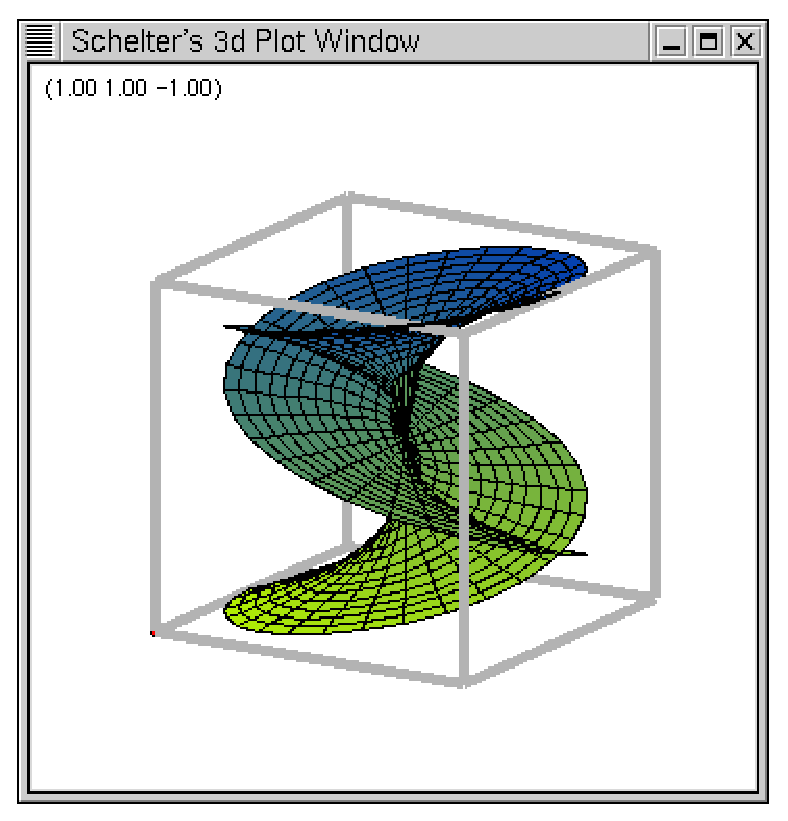
\includegraphics{images/3dplotwindow} \par }

~

Notice in the latter shot the control menu is visible - this appears if you move the mouse to the upper left hand corner of the plot window, and will allow you to configure things like printing options.

\section{Plot Options}



Maxima defines a list, called \verb@PLOT_OPTIONS@, which controls most of the behavior of Maxima's plotting options.  There are two ways of setting these options - you can set an option globally, using the \verb@SET_PLOT_OPTION@ command \footnote{Setting an option globally only changes the option for the current Maxima session - upon restart, the original defaults will be restored.}, or supply the new options as arguements to a plot command.  If you want to check what your global options are currently set at, you can just type \verb@PLOT_OPTIONS;@ and the current state of the system will be listed.

\beginmaximasession
PLOT_OPTIONS;
\maximasession
(C1) PLOT_OPTIONS;

(D1) [[x, - 3, 3], [y, - 3, 3], [GRID, 30, 30], [VIEW_DIRECTION, 1, 1, 1], 

[COLOUR_Z, FALSE], [TRANSFORM_XY, FALSE], [RUN_VIEWER, TRUE], 

[PLOT_FORMAT, OPENMATH], [NTICKS, 100]]
\endmaximasession

OK, let's look at each of these options.

\begin{itemize}
  \item \verb@[x, - 3, 3]@ - This defines the X range.  In order to change this range globally, use a command of the form \verb@SET_PLOT_OPTION([x,-5,5]);@
  \item \verb@[y, - 3, 3]@ - This defines the Y range.  In order to change this range globally, use a command of the form \verb@SET_PLOT_OPTION([y,-5,5]);@
  \item \verb@[GRID, 30, 30]@ - This controls, in 3D plotting, the number of points used to draw the figure.  The function is only calculated at a certain number of points - after that, linear approximations are drawn. Globally, usee a command of the form \verb@SET_PLOT_OPTION([GRID,40,35]);@
  \item \verb@[VIEW_DIRECTION, 1, 1, 1]@ - This option is specific to the case
  when the plot command outputs directly to postscript in 3D(See
  \verb@PLOT_FORMAT@.)  It determines the direction from which the 'camera'
  looks at the function, which is along a line parallel to the line from
  \verb@VIEW_DIRECTION@ to the origin.  It only needs to be set in the case of
  postscript output; it is ignored otherwise.  Globally, use a command of the
  form \verb@SET_PLOT_OPTION([VIEW_@ \verb@DIRECTION,1.4,1.4,1.4]);@
  \item \verb@[COLOUR_Z, FALSE]@ - This refers also to the postscript output - if set to TRUE it provides a little color shading in the output. Form is \verb@SET_PLOT_OPTION([COLOUR_Z, TRUE]);@
  \item \verb@[TRANSFORM_XY, FALSE]@ - This appears to provide the ability to produce plots with different coordinate systems, but I am unsure of how to make it work.  Need to get help here.
  \item \verb@[RUN_VIEWER, TRUE]@ - If you only wish Maxima to output the openmath file and not launch the graphical viewer, set this option to false.  Remember, however, that if you wish to run multiple commands to generate data you will have to recover the information from the maxout.openmath file each time, because each new plot command will overwrite it. Form is \verb@SET_PLOT_OPTION([RUN_VIEWER, FALSE]);@
  \item \verb@[NTICKS, 100]@ - Controls the number of points used to draw the 2D plots - the program will calculate the value of the function at N points, and then draw lines between them.  Form is \verb@SET_PLOT_OPTION([NTICKS, 200]);@
  \item \verb@[PLOT_FORMAT, OPENMATH]@ - This controls which program gets the output from Maxima for display.  There are currently four viable options - OPENMATH, GNUPLOT, GEOMVIEW, and PS.  PS is simply direct output to a postscript file, maxout.ps.  All of these programs are freely available.  
  Geomview is currently Unix only, and is available at
  http://geomview.sourceforge.net as both source and binary.  Openmath is
  distributed as part of Maxima.  Gnuplot is widely available, with a homepage
  at http://www.gnuplot.org and the most current development version at
  http://sourceforge.net/projects/gnuplot.  Gnuplot can run on both Windows and
  Linux. 
  \end{itemize}

\begin{figure}

\centering 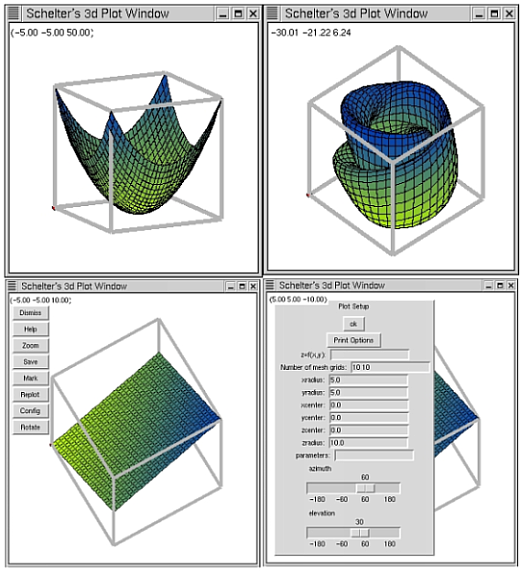
\includegraphics{images/maxima_openmath} \par
\caption{Graphing with Openmath, the default Maxima plotting tool}

\end{figure}

\begin{figure}

\centering 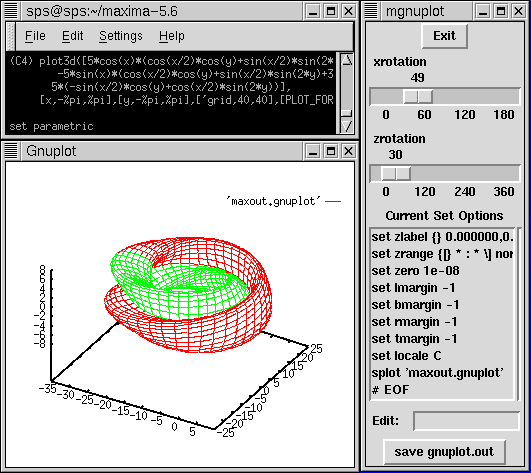
\includegraphics{images/maxima_gnuplot} \par
\caption{Graphing with gnuplot, using the mgnuplot utility}

\end{figure}


\begin{figure}

\centering \includegraphics{images/maxima_geomview} \par
\caption{Graphing with GeomView.}

\end{figure}




\chapter{Maxims for the Maxima User}
  \label{maxims}

Some beginning users of algebraic manipulation systems
find that their
previous experiences with traditional programming systems do
not translate easily into algebraic programming; others find
\Max\
descriptions inadequate because the emphasis is on
the mixture of mathematical notations and algorithms, and not on 
{\it efficient} use of machine or human resources (no one likes to wait
longer than necessary for an answer!).
While we cannot provide a complete education in efficient and effective
programming,
we have collected a few
{\it maxims} in an attempt to help you with some of these {\it start-up}
problems.

\begin{quote}
{\it Algebraic manipulation is a new and different
computational approach for which prior experience with
computational methods may be misleading.
You should attempt to learn the ways in which algebraic
manipulation differs from other approaches.}
\end{quote}


For
example, consider the problem of inverting an $n \times n$
matrix.  In numerical analysis we learn that the problem
requires on the order of $n^3$ operations.  Theoreticians
will point out that for $n$ sufficiently large, one can
reduce the number of multiplications below $ n^3$ to $n^{2.8}$.
This analysis is unfortunately not relevant in dealing with matrices
with symbolic entries.  Consider the number of terms in
the determinant of the general $n \times n$ matrix whose elements
are the symbols $ a_{i,j} $.  When the inverse is written out
in a fully expanded form, just the
determinant (a necessary part of representing
the inverse) has $n !$
terms. It is impossible to compute this determinant in less than {\it time
proportional to $n !$}  In fact,
for large $n$, it is just not feasible
to compute this form explicitly on existing computers.
The combinatorial
or exponential character that some algebraic manipulation
problems have when they are approached with an inefficient algorithm, makes for a vastly
different game from, say, numerical computation, where the size of objects
is generally known at the onset of the calculation, and does not increase.

\begin{quote}
{\it Needlessly generalizing a problem usually results in unnecessary expense.}
\end{quote}

For example, if you wish to obtain determinants
for a collection of matrices whose general
pattern of entries is represented by parametric formulas,
you might consider obtaining the determinant
of the general matrix and substituting various values for the parameters
into the 
result.  This may work for matrices of low order, but
is probably a poor plan for dealing with the exponential
growth inherent in computing symbolic determinants. It would probably
be better to substitute the parameters first, since this would
drastically reduce the cost of the determinant calculation.

Sometimes, when humans are dealing with formulas, it is
preferable to use an indeterminate, say $G$ in a formula 
which is really known to be, say, 3/5.  On the other
hand, it is likely (although not certain!) that the calculation
using 3/5 will take less time than the calculation with $G$.
Since the cost inherent in some computations is usually
a function
of the number of variables in the expression, {\it it pays to reduce the
number of variables in a problem as much as possible.}

\begin{quote}
{\it You should be aware of the types of calculations which in the general
case have exponential growth} (e.g. many matrix calculations with symbolic
entries, repeated differentiation of products or quotients, solution of systems
of polynomial equations).
\end{quote}


\begin{quote}
{\it Your should anticipate a certain amount of trial-and-error in calculations.} 
\end{quote}
Just as in other problem-solving activities,
often the first technique that comes to mind is not the best.  While it
occasionally happens that brute force carries the day, cleverness in computing
can be as important as cleverness in hand calculations.
It is natural, during hand calculations, to apply critical simplificiations
or substitutions in computations. These simplifications include
collecting terms selectively or striking out terms which do not ultimately
contribute to the final answer because of physical interpretations.
Computer algorithms which do not incorporate these same tricks may bog down
surprisingly soon.  Thinking about these shortcuts may be important. In fact,
it is one of the more
rewarding aspects of computer algebra systems that they give the problem solver
an opportunity to organize, encapsulate and distribute
a particularly clever piece of mathematical manipulation.


\begin{quote}
{\it Try to reduce your problem so that it can be performed in a simpler 
domain.}
\end{quote}
For example, if your problem appears to involve trigonometric functions, logs,
exponentials, etc. see if you can reduce it to a rational function (ratio of
polynomials) problem.
If it appears to be a rational function, see if you can, by substitutions,
make it into a polynomial problem, or a truncated power-series problem.
If it appears to be a problem involving rational numbers, consider the use of
floating-point numbers as an alternative, if the growth in the size of numbers
presents difficulties.

There are other special forms that are especially efficient.  In a number
of areas of investigation %
{\it it pays to convert all expressions to the internal rational form
(using  {\tt rat}) or into Poisson-series form (using {\tt intopois}) to
avoid the overhead the the general representation}.
The price you may
pay here is thtat the structure of the formulas may be significantly different
from those you began with:  The canonical transformations used by these
representations drastically re-order, expand, and modify the original expressions.


\begin{quote}
{\it Sometimes someone else has already started on your problem.}
\end{quote}
You should look through the {\it share} directory programs available to see
if there are contributed packages that might be of use either as subroutines or as
models for programming.  You should also consider writing programs that
you develop in solving your problems in a form suitable for sharing with
others.


\begin{quote}
{\it Pattern matching allows you to {\it tune} the system simplifier to your
application, and develop rule-replacement programs}. 
\end{quote}

Learning to use
the pattern-matching facilities effectively is a nontrivial task.  Nevertheless
if you have a fairly complex problem involvilng the recognition and application
of identities, you should consider making an effort to use these facilities.
In recent years, advocates of {\it rule-based expert systems} have claimed
that this type of formalism can or should be used to incorporate varied types of
knowledge.  Algebraic manipulation programs have depended on pattern matching
since at least 1961, for some of their power.


Finally, we would like to point out that algebraic manipulation systems,
in spite of their pitfalls, can be of major assistance in solving difficult
problems.  If you are willing to invest some time in learning, there may be
enormous benefits in using such a system.  We think it is unfortunate that
some users reserve \Max\ for difficult problems.  Those of us who have 
grown up with \Max\
near at hand find it of great use in routine computations as well.


\chapter{Help Systems and Debugging}

    Using the debugger and the online help system.

\chapter{Troubleshooting}

    Common errors, their cause and solution.

\chapter{Advanced Examples}

    These examples try to draw on everything in the manual to show you
    what can be done with Maxima in advanced usages. 
    This is NOT a good starting point for new users.

   %-*-EMaxima-*-

\subsection*{Establishing a Minimum for the Rayleigh Quotient}

We begin by defining the Rayleigh Quotient in general.  From basic
Regular Sturm-Liouville Eigenvalue principles, we know that the 
Rayleigh Quotient is defined as

\[\lambda =\frac{-p\phi \left. \frac{d\phi }{dx}\right| ^{b}_{a}+\int _{a}^{b}\, \left[p \left( \frac{d\phi }{dx}\right)^{2}-q\phi ^{2}\right] \, dx}{\int _{a}^{b}\, \phi ^{2}\sigma \, dx}\]


given the Sturm-Liouville differential equation

\[\frac{d}{dx}\left( p\left( x\right) \frac{d\phi }{dx}\right) +q\left( x\right) \phi +\lambda \sigma \left( x\right) \phi =0\]


where $a<x<b$.

\beginmaxima
RQ:(-p*('ev('ev(u(x)*'diff(u(x),x)),x=a)-'ev('ev(u(x)*diff(u(x),x)),x=b))+
'integrate(p*'diff(u(x),x)^2-q*u(x)^2,x,a,b))/'integrate(u(x)^2*sigma,x,a,b);
\maximatexoutput
{\small$$  {{\int_{a}^{b}{p\*\mathrm{\%DERIVATIVE}^{2}\left(\left(u\left(x
 \right),\linebreak[0]x,\linebreak[0]1\right)\right)-q\*u^{2}\left(
 \left(x\right)\right)\;dx}-p\*\left(\mathrm{EV}\left(\mathrm{EV}
 \left(u\left(x\right)\*\left({{d}\over{d\*x}}\*u\left(x\right)
 \right)\right),\linebreak[0]x=a\right)-\mathrm{EV}\left(\mathrm{EV}
 \left(u\left(x\right)\*\left({{d}\over{d\*x}}\*u\left(x\right)
 \right)\right),\linebreak[0]x=b\right)\right)}\over{\sigma\*\int_{a
 }^{b}{u^{2}\left(\left(x\right)\right)\;dx}}} $$
}
\endmaxima

Now we evaluate it.  This must be done in stages, otherwise the ev command
will not understand its arguements.

\beginmaxima
ev(RQ,p=1,q=0,sigma=1,u(x)=x-x^2,a=0,b=1);
ev(%,diff,integrate);
ev(%,ev);
\maximatexoutput
{\small$$   {{\mathrm{EV}\left(\mathrm{EV}\left(\left(x-x^{2}\right)\*\left(
 {{d}\over{d\*x}}\*\left(x-x^{2}\right)\right)\right),\linebreak[0]x=
 1\right)-\mathrm{EV}\left(\mathrm{EV}\left(\left(x-x^{2}\right)\*
 \left({{d}\over{d\*x}}\*\left(x-x^{2}\right)\right)\right)
 ,\linebreak[0]x=0\right)+\int_{0}^{1}{\mathrm{\%DERIVATIVE}^{2}
 \left(\left(x-x^{2},\linebreak[0]x,\linebreak[0]1\right)\right)\;dx}
 }\over{\int_{0}^{1}{\left(x-x^{2}\right)^{2}\;dx}}} $$
}
$$   30\*\left(\mathrm{EV}\left(\mathrm{EV}\left(\left(1-2\*x\right)
 \*\left(x-x^{2}\right)\right),\linebreak[0]x=1\right)-\mathrm{EV}
 \left(\mathrm{EV}\left(\left(1-2\*x\right)\*\left(x-x^{2}\right)
 \right),\linebreak[0]x=0\right)+{{1}\over{3}}\right) $$
$$   10 $$
\endmaxima

This can be checked by hand.  Seeing that it is correct, we now can use it to 
search for the minimum eigenvalue on a more difficult problem:

\beginmaxima
ev(RQ,p=1,q:-(x^2),sigma=1,u(x)=x-1,a=0,b=1)$
ev(%,diff,integrate)$
EV(%,EV,NUMER);
\maximatexoutput
$$   6.1 $$
\endmaxima

\beginmaxima
ev(RQ,p=1,q:-(x^2),sigma=1,u(x)=-2*x^2+2,a=0,b=1)$
ev(%,diff,integrate)$
ev(%,ev,NUMER);
\maximatexoutput
$$   2.642857142857143 $$
\endmaxima

\beginmaxima
ev(RQ,p=1,q:-(x^2),sigma=1,u(x)=x^3+x^2-2,a=0,b=1)$
ev(%,diff,integrate)$
ev(%,ev,NUMER);
\maximatexoutput
$$   2.776084010840108 $$
\endmaxima

The smallest eigenvalue must therefore be less than or equal to 2.642857...

\subsection*{Laplacian in Different Coordinate Systems}

This will probably go in the main documentation somewhere, but for now I'll
stick it here.

It is possible to express the Laplacian in different coordinate 
systems, provided you know how to define the coordinate system.
We will use Spherical Coordinates for our first example:

\beginmaxima
load(vect)$
scalefactors([[rho*cos(theta)*sin(phi),rho*sin(theta)*sin(phi),rho*cos(phi)],rho,theta,phi]);
depends(f,[rho,theta,phi]);
express(laplacian(f));
ev(%,diff)$
ratexpand(%);
\maximatexoutput
\p  Warning - you are redefining the MACSYMA function TRIGSIMP
Warning - you are redefining the MACSYMA function IMPROVE
Warning - you are redefining the MACSYMA function UPDATE \\
$$   \mathrm{DONE} $$
$$   \left[ f\left(\rho,\linebreak[0]\vartheta,\linebreak[0]\varphi
 \right) \right]  $$
$$   {{{{d}\over{d\*\rho}}\*\left({{d}\over{d\*\rho}}\*f\*\left| 
 \sin \varphi\right| \*\rho^{2}\right)+{{d}\over{d\*\vartheta}}\*{{{{
 d}\over{d\*\vartheta}}\*f\*\left| \sin \varphi\right| }\over{\sin ^{
 2}\varphi}}+{{d}\over{d\*\varphi}}\*\left({{d}\over{d\*\varphi}}\*f
 \*\left| \sin \varphi\right| \right)}\over{\left| \sin \varphi
 \right| \*\rho^{2}}} $$
$$   {{2\*\left({{d}\over{d\*\rho}}\*f\right)}\over{\rho}}+{{{{d
 }\over{d\*\varphi}}\*f\*\cos \varphi}\over{\sin \varphi\*\rho^{2}}}+
 {{{{d^{2}}\over{d\*\vartheta^{2}}}\*f}\over{\sin ^{2}\varphi\*\rho^{
 2}}}+{{{{d^{2}}\over{d\*\varphi^{2}}}\*f}\over{\rho^{2}}}+{{d^{2}
 }\over{d\*\rho^{2}}}\*f $$
\endmaxima


\part{External, Additional, and Contributed Packages}


\chapter{The Concept of Packages - Expanding Maxima's Abilities}

    This chapter will try to give some in depth information on the why
    and how of Maxima packages. It is true that many {}``standard''
    abilities of Maxima, such as vectors, are due to packages, but this
    part of the book will deal with more specialized contributed packages,
    such as elliptical integrals, special scientific packages, etc. That
    way the first part of the book can be rewritten less frequently, but
    we can still have all the information here.


\chapter{Available Packages for Maxima}

    Maybe we can do this in one chapter, maybe each package will warrant
    a chapter. Not sure. For now, I'll assume one Section per package,
    not one Chapter.

\addcontentsline{toc}{chapter}{List of Figures}
\listoffigures

%\addcontentsline{toc}{chapter}{List of Tables}
%\listoftables

\addcontentsline{toc}{chapter}{Index}
\printindex

\addcontentsline{toc}{chapter}{Bibliography}
\bibliography{maxima}
\bibliographystyle{alpha}
\nocite{*}

\end{document}
